%% TO DO:
%% TITOLO CAP 6
%% TABLE OF CONTENTS
%% BIBLIOGRAPHY STYLE
%% GRAFICO CONVERGENCE DT hartris

\documentclass[krantz2,a4paper,11pt,ChapterTOCs,twoside,openright]{krantz}
%\usepackage{fixltx2e,fix-cm}
\usepackage[utf8]{inputenc}
\usepackage[english]{babel}
\usepackage{csquotes}
%\usepackage{lmodern}  % allows flexible font sizes
\usepackage{amssymb}
\usepackage{amsmath}
\usepackage{amsthm}
\usepackage{graphicx}
\usepackage{subfigure}
%\usepackage{makeidx}
\usepackage[bottom]{footmisc} % places footnotes at page bottom
\usepackage{bm}
%\usepackage{multicol}
%\usepackage{textgreek}
%\usepackage[normalem]{ulem}	  % for strike-through of text with \sout{}

%% PAGE LAYOUT
%\usepackage{showframe}
%\widowpenalty=300  % penalties for widow lines
%\clubpenalty=300
\frenchspacing
\tolerance=5000

%% TABLES
%\usepackage{longtable}
%\usepackage{booktabs}
\usepackage{array}
\renewcommand{\arraystretch}{1.2}

%% FIGURES
\usepackage[section]{placeins}  % place floats within section
\usepackage[]{caption}
%\usepackage[labelfont={small,bf},textfont=small]{caption}
\renewcommand{\captionfont}{\fontsize{10}{12}\selectfont}
\renewcommand{\captionlabelfont}{\bfseries\fontsize{10}{12}\selectfont}
\captionsetup{width=0.9\textwidth}
%\usepackage{subcaption}

%% BIBLIOGRAPHY
%\usepackage[numbers,sort&compress]{natbib}

\usepackage[backend=biber,style=phys,sorting=none,hyperref=true,articletitle=true,doi=true,biblabel=brackets,chaptertitle=true,pageranges=false]{biblatex}
%\renewcommand{\bibfont}{\small}  % customized bibliography style
%\setlength{\bibitemsep}{5pt}
\newcommand{\printpublication}[1]{\AtNextCite{\defcounter{maxnames}{99}}\fullcite{#1}}
\addbibresource{bibliography.bib}


%% PDF STUFF
\usepackage{url}
%\usepackage{colortbl}
\usepackage{hyperref}
%\usepackage[inner,right]{showlabels}

%% EDITOR COMMANDS
%\usepackage[usenames,dvipsnames]{color}
%\newcommand{\editor}[2]{%
%  \expandafter\newcommand\csname #1note\endcsname[1]{%
%    \textcolor{#2}{(\textbf{#1:} \emph{\textsf{##1}})}}%
%  \expandafter\newcommand\csname #1\endcsname[1]{%
%    \textcolor{#2}{##1}}%
%  \expandafter\newcommand\csname #1cancel\endcsname[1]{%
%    \textcolor{#2}{\sout{##1}}}%
%  \expandafter\newcommand\csname #1change\endcsname[2]{%
%    \textcolor{#2}{\sout{##1} ##2}}%
%  \newenvironment{#1text}{\color{#2}}{\color{black}}
%}
%\definecolor{blue}{rgb}{0,0.4,0.7}
%\definecolor{tangerine}{rgb}{0.944,0.522,0}
%\definecolor{verde}{rgb}{0,0.5,0}
%\editor{LE}{blue}
%\editor{SB}{tangerine}

%% TABLE OF CONTENTS
%\makeindex
\setcounter{tocdepth}{2}

%% DEFINITIONS
\newtheorem{theorem}{Theorem}
\newtheorem{lemma}{Lemma}
\DeclareMathAlphabet\mathbfcal{OMS}{cmsy}{b}{n}  % bold mathcal letters
\newcommand{\hbindex}[1]{\hl{#1}\index{#1}}  %highlights index entries
\def\smallgamma{{\scriptscriptstyle \gamma}}
\def\smallone{{\scriptscriptstyle 1}}
\def\smallE{{\scriptscriptstyle E}}
\def\smallQ{{\scriptscriptstyle Q}}
\def\smallZ{{\scriptscriptstyle Z}}
\def\smallXC{{\scriptscriptstyle XC}}
\def\smallDFT{{\scriptscriptstyle DFT}}
\def\smallGGA{{\scriptscriptstyle GGA}}
\def\smallH{{\scriptscriptstyle H}}
\def\smallKS{{\scriptscriptstyle KS}}
%\def\eqref#1{(\ref{#1})}
\def\angstrom{{\mbox{\AA}}}
\def\S1{{\mathbb{S}_1}}
\newcommand{\un}[1]{\,\mathrm{#1}}
%\newcommand{\red}[1]{\textcolor{red}{#1}}
\def\rGamma{{\mathrm\Gamma}}
\def\rDelta{{\mathrm\Delta}}
\def\rLambda{{\mathrm\Lambda}}
\def\rOmega{{\mathrm\Omega}}
\def\abinitio{\emph{ab initio} }

%%%%%%%%%%%%%%%%%%%%%%%%%%%%%%%%%%%%%%%%%%%%%%%%%%%%%%%%%%%%%%%%%%%%%%%%%%
\begin{document}

\frontmatter
\title{ab initio simulation of heat transport in silica glass}
\author{Loris Ercole}
%\maketitle
\begin{titlepage}
\begin{center}

  \voffset 1. cm

%%%Upper part of the page
%
 \begin{figure}[h]
 %\vskip 0.6cm
 \centering
 
\includegraphics[width=5.5cm]{frontmatter/SISSA_40_alt.png}
 \end{figure}
\vskip 0.5 cm
\textsc{\Large Scuola Internazionale Superiore di Studi Avanzati}\\ %[0.5cm]

\vskip 1.5 cm
\textsc{\fontsize{10}{12} PhD course in Theory and Numerical Simulation of Condensed Matter}

\vskip 1.4 cm
\hrule height 1.1 pt
\vskip 1.4 cm
%%%Title
% { \Huge \bfseries  Aspetti di Meccanica Quantistica Supersimmetrica}\\[0.4cm]
{ \fontsize{20}{22} \bfseries  \emph{ab initio} Simulation of Heat Transport \\
\vspace{0.4cm}
in Silica Glass
}

\vskip 5.4 cm
{A thesis submitted for the degree of \textit{Doctor Philosophiae}}
\vskip 1.5 cm


\begin{flushleft} \normalsize
\emph{Supervisor}\\
Prof. ~Stefano  \textsc{Baroni}
\end{flushleft}
\vspace{-42 pt}
\hspace{9.6cm}
\begin{minipage}{4.2cm}
%%% \vskip 2.cm
\begin{flushleft} \normalsize
\emph{Candidate} \\
Loris  \textsc{Ercole}
\end{flushleft}
\end{minipage}
%%%% \vskip 1.595 cm
\vspace{1.5cm}
\hrule height 1.1 pt
\vskip 0.3cm
\textsc{\large Academic year 2017/2018}
%%\vfill

%%%Bottom of the page
%%%{\large \today}

\end{center}

\end{titlepage} 
\cleardoublepage
\thispagestyle{empty}
\vspace*{\stretch{1}}
\begin{flushright}
\Large\itshape
To my parents.
\end{flushright}
\vspace{\stretch{3}}
\cleardoublepage
\chapter*{Ringraziamenti}

Ricordo ancora, meno di quattro anni fa, il momento in cui iniziai ad avventurarmi in questo misterioso universo del trasporto termico. Mai avrei immaginato che in pochi anni questo progetto si sarebbe sviluppato e ramificato in così tanti e variegati aspetti, sia pratici, rivelatisi tutt'altro che banali e scontati, sia fondamentali, con inaspettati fondamenti teorici che stanno tutt'ora venendo a galla e che non smettono di affascinarmi. 
Senza dubbio, tutto questo percorso di ricerca non sarebbe stato possibile senza la guida e il sostegno del mio supervisor, Stefano Baroni, a cui va la mia profonda stima e gratitudine. È grazie a lui se mi sono appassionato a questo tema e alla ricerca. 

Devo un grosso ringraziamento anche ad Aris Marcolongo, con cui ho collaborato in molti aspetti di questo lavoro, e a Federico Grasselli e Riccardo Bertossa, con cui ho condiviso gli ultimi due anni del mio soggiorno alla SISSA, per le innumerevoli discussioni in macchina tra Trieste e Verona, e per l'aiuto e l'ispirazione in molteplici problemi.

Quattro anni a Trieste sono passati in un lampo, e questo lo devo interamente a tutti gli amici che hanno condiviso con me questo viaggio, chi prima o chi dopo, sono riconoscente a tutti voi: 
Mariami, Maja, Leyla, Sara, Federico, Riccardo, Ivan, Luca, Francesco, Simone, Tommaso, Caterina, Seher, Nina, Matteo, Juraj, Mattia, Stefano, Tommaso, Francesco, Nicolò, Lorenzo, Federico, Marco, e molti altri.

Nondimeno, devo ringraziare tutti gli amici di Verona, che pur vedendo sporadicamente, mi fanno sempre sentire a casa: i miei compagni Agorà, con cui abbiamo raggiunto traguardi incredibili (e spero sia solo l'inizio!), gli amici di mille più imprevedibili avventure, e gli amici storici su cui puoi sempre contare e che ho sempre il piacere di rincontrare. 

Infine, il ringraziamento più grande va alla mia famiglia e in particolare ai miei genitori, a cui dedico questo lavoro, e senza i quali non avrei davvero potuto raggiungere questo traguardo. \textbf{GRAZIE!}

\cleardoublepage
%\setcounter{page}{7} %previous pages will be reserved for frontmatter to be added in later.

\tableofcontents
% \chapter*{Symbols}
\begin{symbollist}{000000}
\symbolentry{$\alpha$}{To solve the generator maintenance scheduling, in the  past, several mathematical techniques have  been applied.}
\symbolentry{$\sigma^2$}{These include integer programming, integer linear programming, dynamic programming, branch and bound etc.}
\symbolentry{$\sum$}{Several heuristic search algorithms have also been developed. In recent years expert systems,}
\symbolentry{$abc$}{fuzzy approaches, simulated annealing and genetic algorithms have also been tested.}
\symbolentry{$\theta\sqrt{abc}$}{This paper presents a survey of the literature}
\symbolentry{$\zeta$}{ over the past fifteen years in the generator}
\symbolentry{$\partial$}{maintenance scheduling. The objective is to}
\symbolentry{sdf}{present a clear picture of the available recent literature}
\symbolentry{ewq}{of the problem, the constraints and the other aspects of}
\symbolentry{bvcn}{the generator maintenance schedule.}
\end{symbollist}

\mainmatter
\thischaptertocfalse
\chapter{Introduction}  \label{ch:intro}
%\begin{LEtext}
%Struttura del capitolo di intro
%\begin{itemize}
%    \item Intro generale su trasporto termico, importanza nella tecnologia
%    \item difficolta' nel descriverlo, fare modeli: 
%    \item metodi per il calcolo della TC, Green-Kubo method
%    \item ab initio GK - hurdles: gauge invariance, data analysis
%    \item importanza per i vetri, il trasporto termico e' ancora poco capito nei vetri
%    \item esempio: silica glass, importanza della TC, difficolta' coi potenziali classici
%    \item scope of the thesis: tackle these theoretical and practical hurdles, and apply this method to amorphous materials for the first time, to the study of Silica glass
%    \item lista della spesa
%\end{itemize}
%-----
%\end{LEtext}

\vspace{1cm}
\nocite{Ercole2016,Ercole2017,Baroni2018,Bertossa2018}

Heat flow is ubiquitous in nature, it governs a multitude of complex processes, from the evolution of stars and planets to the dynamical stability of biological systems, all the way down to the maintenance of optimal operating conditions in many (nano)technological applications. 
Heat flow determines the internal temperature distribution of out-of-equilibrium systems and the rate of cooling or heating of bodies. 
Therefore the study of thermal transport is fundamental to modeling a multitude of complex systems, and to engineer nanotechnologies, where thermal insulation or dissipation properties have to be properly designed. 
Yet, despite being one the oldest problems of statistical mechanics, a complete theoretical understanding of heat transport is still lacking. 

Transfer of thermal energy occurs via three different mechanisms, that may prevail or coexist in different regimes \cite{Lienhard2017}: \emph{convection}, in which heat is transported by a flow of mass; \emph{radiation}, in which heat is removed from the surface of the hot source by photons; and \emph{conduction}, in which heat transfer is determined by the microscopic dynamics of atoms, or in the case of metals, of conduction electrons. 
In condensed phases and at the molecular scale, conduction is by far the most relevant heat transfer mechanism, and we shall focus on it. 
The first macroscopic theory of heat transport was formulated by Fourier \cite{Fourier1878}, in 1822, who established a proportionality law between the heat current $\mathbf{J}$ and the temperature gradient in the system $\nabla T$:
\begin{equation}
    \mathbf{J} = -\kappa\, \nabla T \,.  \label{eq:Fourier-law}
\end{equation}
The ratio between the heat flux and the temperature gradient defines the \emph{thermal conductivity}, $\kappa$, which is an intrinsic property of the material. 

\medskip

\paragraph{Glass, a quintessential nanotech man-made material}
Although being known and used for more than two thousand years, the last century experienced extraordinary advances in the definition, fabrication, characterisation, and application of glass \cite{Mauro2014}. 
Methods and theory analogous to those employed in the study of crystalline solids have been used to study the electronic, atomic, and micro-structural properties of glass, trying to describe the basic nature of the glassy state, that still represents one of the most difficult open problems in science \cite{MauroFM14}. 
An increased understanding and control of the structure of glass, with both fundamental and fabrication advances, has led to remarkable applications in a variety of fields such as civil engineering, transportation, electronics, photonics, communication, and medicine, many of which are today accepted as the norm. 
Glass is more and more demanded as a high-tech material for consumer electronic devices, and it is going to play a critical role in solving several of the global energy and healthcare challenges of today. 

An atomic-level description of the glassy state is extremely complex due to the lack of long-range order found in crystalline materials, and to the intrinsic non-equilibrium nature of this material. However, thanks to the recent theoretical and experimental advances, glass science is maturing from an empirical discipline to one built upon rigorous scientific principles. 
The glass transition and the processes involved in glass formation are still open questions. 
The chemistry of glasses can be extremely complex: glass compositions are infinitely tunable in chemistry, allowing one to design glasses with tailored mechanical, optical, electrical, magnetic, and thermal properties for specific purposes. 
However this task is far from easy. For example, it was recently discovered that two glasses of identical chemistry may exhibit considerably different short-range structural ordering, thus leading to large differences in the observed properties, a phenomenon called polyamorphism \cite{Huang2004,McMillan2004}. 

In particular, the thermal conductivity is a fundamental property for many industrial and technological applications of glass, ranging from electronics to the insulation efficiency of windows for green architectures, to nuclear waste storage. Despite its importance, ``\emph{thermal conductivity of glass represents largely unexplored territories, ripe for new research efforts}'' (J. Mauro, senior research manager -- Glass Research, Corning Inc.) \cite{MauroFM14}. 
The understanding of thermal conductivity and its structural origin in glasses has been greatly overlooked in the literature and presents several non trivial challenges for atomistic simulations. 
The problem of generating faithful amorphous structures and the correct description of the vibrational properties are the key points that one needs to solve to estimate the thermal conductivity of glasses. 
Moreover, non-periodic systems still lack a theory able to describe the contributions to the thermal conductivity in a way similar to methods widely used for crystalline solids. 



\paragraph{Vitreous silica}
Vitreous silica (a-SiO$_2$, aka fused silica or fused quartz) and silicate glasses in general have been the subject of significant research efforts in the last decades, due to their many technological applications that range from thermal insulation to laser engineering, semiconductor fabrication, and optical communication.
In particular, thanks to its excellent UV transparency, mechanical stability, and chemical durability, silica can be used in many optical applications, such as the diffractive elements and the protective windows of the optics assemblies of inertial confinement fusion facilities. In these facilities, extremely intense nanosecond laser pulses are used and can seriously challenge the durability the optical glasses. It is indeed well established that the small defects or impurities of the glass may cause local lattice heating and melting, resulting in damage craters that will rapidly degrade its optical performance \cite{Miller2004,Canaud2004,Miller2010,Chambonneau2014,Kuzuu1999,Stuart1995,Wong2006,Carr2010,Saito2000}. Moreover, these local damages can be mitigated by using pulsed laser treatments that increase the damage sites to temperatures of $2000-5000\un{K}$ in $10^{-9}$ down to $10^{-12}\un{s}$ and partially restore the desired optical properties \cite{Soules2011}. 
The interpretation of these types of damage processes require the study of thermal properties and the prediction of the thermal conductivity of silica glass, especially in these extreme conditions that experiments cannot probe.

Furthermore, amorphous silica serves as the basis of multicomponent silica glasses, that are adopted for a wide range of special applications. 
To cite an example, borosilicate glasses (BSG) are broadly used to vitrify and immobilize high-level nuclear waste, forming a stable solid matrix that is then stored for very long time \cite{OjovanBook13}. These glasses proved to be one of the most reliable materials to accomplish this task, indeed their intrinsic disorder reduces the effects of radiation damage and their chemical stability and resistance to water corrosion ensures a long and safe storage. A high thermal conductivity favours the efficiency of the fabrication and the stability of the final product, as it entails a faster dissipation of heat generated by radioactive decays. 
Predicting the thermal conductivity of silica also represents the first step towards the prediction of the thermal conductivity of more complicated glasses such as BSG, whose components are characterised by a complex chemistry that is more difficult to model. 

Silica glass has been the subject of many classical MD studies in the last twenty years, that showed that classical force fields can reproduce reasonably well all the structural properties of a-SiO$_2$, but do not describe very well its vibrational spectrum, that instead requires first-principles simulations. 
Its thermal conductivity, that depends on both these properties, still lacks satisfactory and reliable calculations and thus calls for a rigorous study to finally settle the issue. 
Besides, silica also lacks a proper study determining dependence of $\kappa$ on some simulation factors, such as the cooling protocol used to prepare the glass sample and that influences remarkably its structural properties, and the size of system. 


\paragraph{Computing thermal conductivity}
Notwithstanding its fundamental importance, ``\emph{thermal conductivity has proven to be one of the most difficult transport coefficients to calculate}'' \cite{Evans1990} and its simulation is still today a conceptual, no less than practical, challenge to our materials modeling capabilities. 
In order to compute $\kappa$, one needs a microscopic theory that describes the conduction of heat carriers, \emph{i.e.} electrons and lattice vibrations (phonons). Hereafter we will focus only on lattice vibrations, the only carriers contributing to heat transport in \emph{insulators} (the electrons following adiabatically in their ground state), to which we restrict our attention. 
The first microscopic theory of lattice thermal transport was formulated by Peierls, in 1929, and is based on the assumption that phonons obey the Boltzmann transport equation (BTE) \cite{Peierls1929}. 
About thirty years later, Green and Kubo (GK) independently expressed the thermal conductivity, as well as other transport coefficients, by liner response theory in terms of correlation functions of the heat currents \cite{Green1952,Green1954,Kubo1957a,Kubo1957b,Zwanzig1965}:
\begin{equation}
    \kappa \propto \int_{0}^{\infty}\!\langle{J}(t){J}(0)\rangle\, dt, \label{eq:GK-intro}
\end{equation}
where the brackets indicate ensamble averages, thus allowing its computation from simple equilibrium molecular dynamics (MD) simulations. 

In the meantime, a few decades ago, our abilities to understand and predict the properties of materials were boosted by the advent of density functional theory (DFT) \cite{Hohenberg1964,Kohn1965,Martin2008}, which allows computing interactions entirely from quantum mechanics, thus freeing us from the need to leverage prior experimental knowledge, in order to perform MD simulations. 

Recent developments enabled the implementation of the BTE from first principles, thus making it the state of the art technique to compute $\kappa$ of bulk crystalline materials (\emph{e.g.} Si, Ge, diamond \cite{Broido:2007iu,Ward2009}) and nanostructures (\emph{e.g.} graphene and 2D materials \cite{Fugallo2014}). \emph{Ab initio} BTE also provides insights into the mechanisms of heat transport, by breaking down the contributions to $\kappa$ into single carrier properties. 
Nonetheless, the applicability of the BTE approach is limited to periodic materials at low temperatures, where the harmonic approximation of normal modes applies or anharmonic effects are very limited, and it cannot be straightforwardly applied to disordered systems, such as glasses and liquids, were phonons are not even defined, and for which MD is a natural choice. 

On the other hand, MD is set to overcome these limitations: it allows one to study non-periodic and highly anharmonic systems in a straightforward way and to compute their thermal conductivity accounting for full anharmonicity. The only inputs required are the atomic structure and an appropriate interatomic potential, which can be constructed empirically, \emph{e.g.} by fitting previous experimental or \abinitio results using force fields or modern neural networks (classical MD), or directly by first-principles DFT calculations (\abinitio MD, AIMD). 
Once one has these ingredients, $\kappa$ can be computed from equilibrium MD (EMD) or non-equilibrium MD (NEMD) simulations. The latter directly exploits the Fourier law, Eq.~\eqref{eq:Fourier-law}, and applies straightforwardly to finite systems and interfaces, but suffers from severe practical difficulties, such as finite-size and non-linear effects, that have to be carefully accounted for. 
Instead, we focus on EMD simulations, from which the thermal conductivity can be computed directly via the GK equation, Eq.~\eqref{eq:GK-intro}, that only requires an expression for the \emph{heat current}. 
For classical empirical potentials, such expression can be readily obtained as a sum of atomic contributions, containing the atomic coordinates, velocities, and forces. 
On the other hand, a corresponding definition in the framework of DFT was not considered possible until very recently, when it was formulated successfully for the first time \cite{Marcolongo2016}.
Indeed, despite its rigour and simplicity, the GK theory has long been deemed incompatible with DFT, because the total energy cannot be decomposed into individual localized atomic contributions, thus making the heat current ill-defined. 

This conceptual prejudice hindered the development of the GK theory in AIMD simulations for many years. It was only a few years ago that the spurious nature of this belief was recognized through the discovery of a \emph{gauge invariance principle} for transport coefficients \cite{Marcolongo2016,Ercole2016}. 
This principle ensures the value of thermal conductivity ultimately estimated through the GK equation does not depend on the microscopic details that define the energy density, from which the heat current is derived, hence $\kappa$ is well-defined, as any measurable quantity should be. 
However, the problem of univocally defining the atomic energies exists also in classical MD simulations and was recognized in the past, although applications of the GK equation resorted on what was considered the most straightforward definition, without formally justifying this choice. 

On the other hand, despite these important discoveries, experience from classical MD simulations indicates that the practical implementation of the GK theory usually requires very long trajectories to estimate $\kappa$, thus making expensive quantum simulations unfeasible. 
Several expedients have been used in the last twenty years to determine the convergence of the integral in Eq.~\eqref{eq:GK-intro} from trajectories of finite-length, yet it is very surprising that none of these is able to estimate the statistical error of $\kappa$ in an efficient and reliable way. Most of these methods are designed and tested on specific classes of systems, such as crystalline solids (for which, besides, the BTE is the preferable method), but do not work for liquids, disordered or strongly anharmonic systems, or they require extremely long MD simulations. 
We addressed this problem using an innovative data-analysis method based on the \emph{spectral analysis} of stationary time series \cite{Ercole2017}, that provides a rigorous estimation of $\kappa$ with good statistical accuracy from optimally short MD trajectories, for different classes of materials. 
%it is possible to obtain an asymptotically unbiased and consistent estimator for $\kappa$ (\emph{i.e.} the bias and statistical error go to zero in the limit of long simulations). We benchmark it numerically on four different classes of materials and we find that relatively short MD simulations, of the order of one to a few hundreds of picoseconds, are sufficient to obtain a very good statistical error on $\kappa$, of about $\sim 10\%$. 

These two achievements finally demonstrate the feasibility of \abinitio GK simulations of thermal transport and pave the way to their application to previously intractable materials, such as fluids, crystals under extreme conditions, and glasses. 


\medskip

\paragraph{Purpose of this Thesis}
In this thesis we aim to calculate for the first time the thermal conductivity of silica glass at different temperatures, by applying the \abinitio Green-Kubo theory of thermal transport. 
We first show how it is possible to overcome the conceptual and methodological problems mentioned above, that involve the bottom-up definition of a heat current and the estimation of the thermal conductivity from optimally short MD trajectories. 
For this scope, we present the gauge invariance principle for thermal transport coefficients and an innovative data-analysis protocol for transport coefficients. 
We then introduce the problem of simulating an amorphous system with MD, and by means of classical MD simulations we study the effects of sample preparation on the value of thermal conductivity of a-SiO$_2$. 
We use these results as a starting point to run a few first-principles simulations aimed to compute the thermal conductivity of silica at different temperatures using DFT. 

%In the this thesis we present a first application of the \abinitio Green-Kubo theory and the other methodological advances presented. 
%Starting from a classical study, in which we study the effects of many simulation parameters on the thermal conductivity, we then compute $\kappa$ using first-principles simulations at different temperature conditions, and compare the results with experiments. 

\medskip
This thesis is organized as follows. 
Chapter~\ref{ch:green-kubo} introduces the Green-Kubo theory of heat transport. 
Starting from a light review of the theory of hydrodynamic variables and linear response theory, we derive the GK equation for one-component and multi-component systems, and we obtain an expression for the energy current for classical force fields. 
In Chapter~\ref{ch:gauge-invariance} we address the definition of atomic energies and energy densities in interacting systems. We show that there is no unique way to define the heat current, nevertheless the resulting thermal conductivity is well-defined. We prove this statement by numerical simulations and by theory, introducing the principle of gauge invariance of thermal transport coefficients. 
In Chapter~\ref{ch:dft-heat}, after briefly reviewing some of the most recent first-principles simulation techniques of thermal transport, we show how one can derive and compute an \abinitio expression for the energy current in the framework of density functional theory. 
%\LEnote{**discorsi rinormalizzazione**}
Chapter~\ref{ch:data-analysis} is entirely devoted to the practical evaluation of the thermal conductivity from the GK equation. We briefly review all the analysis methods found in the literature, and comment upon their weak points. 
We thus introduce a new technique to evaluate transport coefficients, based on the so-called \emph{cepstral analysis} of time series, and we benchmark it with classical MD simulations for different classes of materials.
In Chapter~\ref{ch:silica} we study the thermal conductivity of a-SiO$_2$ using the \abinitio GK theory. 
We discuss the aspects involved in the atomistic simulation of glass and we simulate silica with classical MD using a popular force field. In particular, we study the dependence of $\kappa$ on the size of the system and the quenching rate used in the virtual vitrification process. 
We then select an optimal system size and simulate one sample with AIMD. 
We compute its thermal conductivity at four different temperatures, and we finally compare the simulation results with experiments. 
Chapter~\ref{ch:conclusions} finally contains our conclusions.

\smallskip
Some parts of Chapter~\ref{ch:green-kubo}, \ref{ch:gauge-invariance}, and \ref{ch:data-analysis} were adapted from the following papers that I have (co-)authored:

\begin{itemize}
    \setlength{\itemsep}{-10pt}
    \item[\textbf{\cite{Ercole2016}}] \printpublication{Ercole2016}. \\
    \item[\textbf{\cite{Ercole2017}}] \printpublication{Ercole2017}. \\
    \item[\textbf{\cite{Baroni2018}}] \printpublication{Baroni2018}. \\
    \item[\textbf{\cite{Bertossa2018}}] \printpublication{Bertossa2018}. \\
\end{itemize}






%\LEnote{**AEROGELS: \small Silica aerogel, a highly porous material first synthesized in the early thirties [1], are currently being produced using a sol–gel process such as hydrolyzing tetramethoxysilane (TMOS) to form silica and methanol, and subsequently dried through supercritical drying together with carbon dioxide [2]. Silica aerogel has several highly desirable properties including being environmentally safe, having high optical transmission as well as large thermal resistance [3]. These properties make silica aerogel very suited for applications such as thermal and acoustic insulation in buildings and appliances, passive solar energy collection devices, and dielectrics for integrated circuits [4]. Also, it is a suitable substitute for chlorofluorocarbon-based plastics in thermal insulation of refrigerators. The most well-known application was in Cherenkov radiators [5] as Cherenkov counters. Another crucial characteristic of aerogels is their extremely low density for a solid, which can go as low as 0.003 g/cm3. Comparatively, the density of air is approximately 0.0012 g/cm3 , which is only three times lower than that of the silica aerogel. This would represent significant weight savings when used in various monolithic structures. **}
  % Introduction
\thischaptertoctrue
\chapter{Green-Kubo theory of heat transport}  \label{ch:green-kubo}

Our microscopic understanding of heat and mass transport in extended systems is rooted in the Green-Kubo (GK) theory of linear response \cite{Green1954,Kubo1957a}, as applied to the Navier-Stokes equations for the densities of the conserved extensive variables \cite{Kadanoff1963,Forster1975}, which include energy, momentum, and the particle numbers for each molecular species. 
\begin{LEtext}

This work was initiated by Onsager in the thirties \cite{Onsager1931a,Onsager1931b} and carried on by Green and Kubo in the fifties with the theory of linear response \cite{Green1952,Green1954,Kubo1957a,Kubo1957b}. The theory is built on the concept of adiabatic decoupling of the slow long-wavelength components of the densities of conserved extensive quantities (which include energy, momentum, and particle number) \cite{Kadanoff1963}, the so-called \emph{hydrodynamic variables}, from the other atomically fast degrees of freedom. Their work resulted in the celebrated \emph{Green-Kubo equations}, a consequence of the fluctuation-dissipation theorem, that establish a relation between a (non-equilibrium) transport coefficient $\kappa$ and the spontaneous fluctuations of the relevant currents $J$ at equilibrium. Transport coefficients are in fact proportional to their autocorrelation times:
\begin{equation}
\kappa\propto\int_{0}^{\infty}\!\langle{J}(t){J}(0)\rangle\, dt, \label{eq:GK}
\end{equation}
where the brackets indicate ensemble averages over trajectories, and are accessible to equilibrium MD simulations.

In this chapter we briefly walk through the theory that allows the derivation of the Green-Kubo equations for transport coefficients, starting from the definition of the hydrodynamic variables of a system. in Section~\ref{sec:hydrodyn_var}, and the use of linear response theory to connect equilibrium properties to non-equilibrium ones, presented in Section~\ref{sec:linear-response}. In Section~\ref{sec:heat-transport}, we then specialize to the case of heat transport in solids and one component fluids, and the particular case of multi-component fluids, and we derive the expression of the energy flux for systems described by classical force fields.
\end{LEtext}


%%%%%%%%%%%%%%%%%%%%%%%%%%%%%%%%%%%%%%%%%%%%%%%%%%%%%%%%%
\section{Hydrodynamic variables} \label{sec:hydrodyn_var}
The macroscopic processes occurring in condensed matter are often described in terms of \emph{extensive variables}. By definition, the value that such a variable assumes for a system is the sum of the values it has for each of its subsystems. This property allows one to express an extensive variable, $A$, as the integral of a suitably defined density, $a(\mathbf{r})$, as:
\begin{equation}
A[\rOmega]=\int_\rOmega a(\mathbf{r})d\mathbf{r}, \label{eq:A-extensivity}
\end{equation}
where $\rOmega$ is the system volume. Here and in the following boldfaces indicate 3D vectors and Greek subscripts label Cartesian components: $\mathbf{u}= \{u_\alpha\} = \{u_1,u_2,u_3\}$. When an extensive quantity is locally conserved, a current density, $\bm{j}(\mathbf{r},t)$, can be associated to its density in such a way that the two of them satisfy the continuity equation:
\begin{equation}
\frac{\partial a(\mathbf{r},t)}{\partial t} = - \nabla\cdot\bm{j}(\mathbf{r},t), \label{eq:continuity}
\end{equation}
where $\nabla\cdot\bm{j}$ indicates partial differentiation and the middle dot a scalar product (a divergence in this case). In the following the densities and current densities of conserved quantities will be called \emph{conserved densities} and \emph{conserved currents} for short. The space Fourier transform of Eq.~\eqref{eq:continuity} reads:
\begin{equation}
\dot{\tilde a}(\mathbf{q},t) = - i\mathbf{q} \cdot \tilde {\bm{\jmath}} (\mathbf{q},t), \label{eq:kontinuity}\end{equation}
where the overdot indicates a time derivative and the tilde a Fourier transform, so that the longer the wavelength, the slower is the dynamics of a conserved density. We conclude that for long enough wavelengths, conserved densities are adiabatically decoupled from all the other (zillions of) fast atomic degrees of freedom. Note that in this chapter we are using the concept of \emph{adiabatic decoupling} in two distinct senses, depending on the context: to indicate the decoupling of electronic from nuclear degrees of freedom, and that of hydrodynamic variables from fast atomic ones.

The long-wavelength Fourier components of conserved densities are called \emph{hydrodynamic variables}. In macroscopically homogeneous systems, different wavelengths are decoupled from each other, while, as we have seen, the long wavelengths are adiabatically decoupled from all the other degrees of freedom. Let us suppose there are $Q$ conserved extensive variables. In the case of a mono-atomic fluid, for instance, $Q=5$, corresponding to mass (or particle number), energy, and the three components of the momentum. In order to simplify the notation, we set the value of the conserved quantities equal to zero, $A^i=0$, so that their densities, $a^i(\mathbf{r})$, directly refer to the departure from equilibrium, and we indicate by $\bm j^i(\mathbf{r},t)$ the corresponding currents. At equilibrium, all the conserved densities and currents vanish. Off equilibrium, it will be assumed that the wavelength and the time scale of the disturbances are so long that thermal equilibrium still holds \emph{locally}. That is to say, a local temperature, pressure, and chemical potential can be defined, such that, when combined with the densities of extensive variable, they satisfy a local equation of state.

For small enough deviations from equilibrium, the time derivatives of conserved densities are linear combinations of the densities themselves. In the frequency/wavevector domains this condition can be expressed as
\begin{equation}
  -i\omega\tilde a^i(\mathbf{q},\omega) = \sum_j \tilde\rLambda^{ij}(\mathbf{q},\omega) \tilde a^j(\mathbf{q},\omega), \label{eq:Fourier-continuity}
\end{equation}
where the tilde indicates now a space-time Fourier transform: $\tilde a(\mathbf{q},\omega) = \int \mathrm{e}^{-i(\mathbf{q}\cdot \mathbf{r}-\omega t)} a(\mathbf{r},t)d\mathbf{r}dt $. By combining Eq.~\eqref{eq:Fourier-continuity} with the time Fourier transform of Eq.~\eqref{eq:kontinuity}, we obtain the so-called constitutive equations for the (longitudinal components of the) conserved currents:
\begin{equation}
  \tilde{\bm{\jmath}}^i(\mathbf{q},\omega)=i\frac{\mathbf{q}}{q^2} \sum_j\tilde \rLambda^{ij}(\mathbf{q},\omega)\tilde a^j(\mathbf{q},\omega). \label{eq:constitutive-qomega}
\end{equation}
In isotropic media, the $\tilde\rLambda$'s are spherically symmetric functions of $\mathbf{q}$, whereas their value at $\mathbf{q}=0$ vanishes, because a non-vanishing value would imply a non-physical long-range dependence of the currents on density fluctuations, in contrast with our assumption of local thermodynamic equilibrium. The long-wavelength low-frequency limit of the coupling constants can thus be assumed to be $\tilde\rLambda^{ij}(\mathbf{q},\omega) \sim q^2 \lambda^{ij}$, so that the macroscopic ($\mathbf{q}=0$) stationary ($\omega=0$) components of the currents, $\mathbf{J}^i = \frac{1}{\rOmega} \int\bm j^i (\mathbf{r}) d\mathbf{r}$, are related to the corresponding components of the density gradients, $\mathbf{D}^i=\frac{1}{\rOmega}\int\nabla a^i(\mathbf{r})d\mathbf{r}$, through the equations:
\begin{equation}
  \mathbf{J}^i=\sum_j \lambda^{ij}\mathbf{D}^j. \label{eq:constitutive}
\end{equation}
In the following, the macroscopic component of a current will be indicated as a \emph{flux}.

Let $x^i=\frac{\partial S}{\partial A^i}$ be the intensive variable conjugate to $A^i$, where $S$ is the system's entropy, and $\chi^{ij} = \frac{1}{\rOmega} \frac{\partial A^i}{\partial x^j}$ the corresponding susceptibility. For instance, when $A^i$ is the energy of the system, the corresponding conjugate variable is the inverse temperature, $x^i=1/T$, while, when $A^i$ represents the number of particles of a given species, one has $x^i= - \mu^i/T$, $\mu^i$ being the corresponding chemical potential. The hypothesis of local thermodynamic equilibrium allows defining local values of the intensive variables, and we define \emph{thermodynamic forces} as their average gradients: $\mathbf{F}^i= \frac{1}{\rOmega} \int \nabla x^i(\mathbf{r})d\mathbf{r}$. The average density gradients are related to the thermodynamic forces through the susceptibility defined above, as:
\begin{equation}
\mathbf{D}^i=\sum_j\chi^{ij}\mathbf{F}^j .
\end{equation}
By inserting this relation into Eq.~\eqref{eq:constitutive}, one gets:
\begin{equation}
\mathbf{J}^i=\sum_j L^{ij} \mathbf{F}^j, \label{eq:onsager}
\end{equation}
where $L^{ij}=\sum_k\lambda^{ik}\chi^{kj}$. Eq.~\eqref{eq:onsager} expresses the linear relation between fluxes, the $\mathbf{J}$'s, and thermodynamic affinities, the $\mathbf{F}$'s, for which Onsager derived his celebrated reciprocity relations ($L^{ji}=L^{ij}$) from microscopic reversibility \cite{Onsager1931a,Onsager1931b,Casimir1945}. Note that, according to our definition, both the $\mathbf{J}$'s and the $\mathbf{F}$'s in Eq.~\eqref{eq:onsager} do not depend on the size of the system.


%%%%%%%%%%%%%%%%%%%%%%%%%%%%%%%%%%%%%%%%%%%%%%%%
\section{Linear-response theory}  \label{sec:linear-response}
In order to evaluate the $L^{ij}$ phenomenological coefficients appearing in Eq.~\eqref{eq:onsager}, we consider a classical system of $N$ interacting atoms described by the Hamiltonian
\begin{equation}
  H^\circ(\rGamma) = \sum_n\frac{1}{2M_n}(\mathbf{P}_n)^2 + V(\mathbf{R}_1,\mathbf{R}_2,\cdots \mathbf{R}_N), \label{eq:unperturbed_H}
\end{equation}
where $M_n$, $\mathbf{R}_n$, and $\mathbf{P}_n$ are the masses, coordinates, and momenta of the $n$-th particle, $\rGamma=\{\mathbf{R}_n,\mathbf{P}_n\}$ indicates the phase-space coordinates of the entire system, and $V$ is a generic many-body potential. Let us now suppose that the system is subject to an external perturbation that can be described as a linear combination of the conserved densities, $\{a^i(\mathbf{r};\rGamma)\}$, as:
\begin{equation}
   V'(\rGamma,t) = \sum_i \int  v^i(\mathbf{r},t) a^i(\mathbf{r};\rGamma) d\mathbf{r}, \label{eq:perturbation}
\end{equation}
where $a(\mathbf{r};\rGamma)$ is a phase-space function whose ensemble average is the conserved density,
\begin{equation}
    \begin{aligned}
      a(\mathbf{r}) &= \langle a(\mathbf{r};\rGamma) \rangle \\
      & = \int a(\mathbf{r};\rGamma) \mathcal{P}^\circ(\rGamma)d\rGamma,
    \end{aligned}
\end{equation}
$\mathcal{P}^\circ(\rGamma) \propto \mathrm{e}^{-\frac{H^\circ(\rGamma)}{k_BT}}$ is the equilibrium distribution, $k_B$ the Boltzmann constant, and $\{v^i(\mathbf{r},t)\}$ are time-dependent fields that couple to the conserved densities and vanish at $t=-\infty$, when the system is assumed to be in thermal equilibrium at some temperature $T$. Of course, conserved currents are also expected values of some phase-space functions, $\bm{j}(\mathbf{r})=\langle \bm{j}(\mathbf{r};\rGamma)\rangle$. The phase-space functions whose expected values are conserved densities/currents will be referred to as \emph{phase-space samples} of the currents/densities. In the following, when the phase-space dependence of a conserved density/current is explicitly indicated, we will mean a phase-space sample; when it is not a phase-space average will be implied. When a phase-space sample is evaluated along a dynamical trajectory, $\rGamma_t$, the sample function will depend on time and on the initial conditions of the trajectory. Averaging with respect to the initial conditions will result in a time-dependent expected value for the conserved densities (or currents):
\begin{equation}
  \begin{aligned}
    a(\mathbf{r},t) &= \langle a(\mathbf{r};\rGamma'_t)\rangle_0 \\
    &= \int a(\mathbf{r};\rGamma'_t) \mathcal{P}^\circ(\rGamma_0) d\rGamma_0.
  \end{aligned} \label{eq:a(r,t)}
\end{equation}
In Eq.~\eqref{eq:a(r,t)} the notation $\rGamma'_t$ denotes somewhat pedantically that the time evolution in phase space is driven by the perturbed Hamiltonian, $H^\circ+V'$. If it were driven by $H^\circ$, evidently the value of $a$ would be time-independent. In the following, the notation $\rGamma_t$ will indicate an unperturbed time evolution. As an example, the phase-space sample of the particle density can be assumed to be $n(\mathbf{r};\rGamma) = \sum_n \delta (\mathbf{r}-\mathbf{R}_n)$, the corresponding current is $\bm{j} (\mathbf{r}, \rGamma) = \sum_n \delta(\mathbf{r}-\mathbf{R}_n) \mathbf{P}_n / M_n $, and a local external potential is described by: $V'(\rGamma,t)=\sum_n v(\mathbf{R}_n,t)=\int v'(\mathbf{r},t) n(\mathbf{r};\rGamma) d \mathbf{r}$. Note that sample functions are not necessarily univocally defined. Different functions whose phase-space averages coincide in the long-wavelength limit sample the same hydrodynamical variable. More on this in Chapter~\ref{ch:gauge-invariance}.

According to Ref.~\citenum{Green1954}, \citenum{Kubo1957a}, and \citenum{Kubo1957b}, the linear response of the $i$-th conserved current to the perturbation is:
\begin{align}
  j_\alpha^i(\mathbf{r},t) & = \frac{1}{k_B T} \sum_j \int_{-\infty}^t dt' \int d\mathbf{r}' \Bigl \langle j_\alpha^i(\mathbf{r},\rGamma_t)\dot a^j(\mathbf{r}',\rGamma_{t'})\Bigr \rangle_0 v^j(\mathbf{r}',t') \\
  &= \frac{-1}{k_B T} \sum_{j,\beta} \int_{-\infty}^t dt' \int d\mathbf{r}' \Bigl \langle j_\alpha^i(\mathbf{r},\rGamma_t) \partial'_\beta j_\beta^j(\mathbf{r}',\rGamma_{t'})\Bigr \rangle_0 v^j(\mathbf{r}',t') \\
  &= \frac{1}{k_B T} \sum_{j,\beta} \int_{-\infty}^t dt' \int d\mathbf{r}' \left \langle j_\alpha^i(\mathbf{r},\rGamma_{t}) j_\beta^j(\mathbf{r}',\rGamma_{t'})\right \rangle_0 \partial'_\beta v^j(\mathbf{r}',t'). \label{eq:linear-response-c}
\end{align}
The second line follows from the first through the continuity equation, Eq.~\eqref{eq:continuity}, while the third line follows after integrating by parts with respect to $\mathbf{r}'$. The notation $\partial'_\beta=\frac{\partial}{\partial r'_\beta}$ has been used.

By integrating Eq.~\eqref{eq:linear-response-c} all over the space, and assuming space-time homogeneity as well as isotropy, one recovers Eq.~\eqref{eq:onsager} with:
\begin{align}
J^i_\alpha(\rGamma) &= \frac{1}{\rOmega} \int j^i_\alpha(\mathbf{r},\rGamma) d\mathbf{r}, \label{eq:J_def}\\
F^i_\alpha(\rGamma) &= \frac{1}{\rOmega T} \int \partial_\alpha v^i(\mathbf{r},\rGamma) d\mathbf{r}, \label{eq:F_def}\\
L^{ij}_{\alpha\beta} &= \frac{\rOmega}{k_B} \int_0^\infty \left\langle J^i_\alpha(\rGamma_t) J^j_\beta(\rGamma_0)\right\rangle_0 dt. \label{eq:L_def}
\end{align}
This completes the derivation of the Green-Kubo formula for transport coefficients, Eq.~\eqref{eq:GK}, from classical linear-response theory. Onsager's reciprocity relations, $L^{ij}=L^{ji}$ \cite{Onsager1931a,Onsager1931b}, follow from Eq.~\eqref{eq:L_def} leveraging time-translational invariance, $\langle J^i_\alpha(\rGamma_t) J^j_\beta(\rGamma_0) \rangle = \langle J^i_\alpha(\rGamma_0) J^j_\beta(\rGamma_{-t}) \rangle$, and micro-reversibility, $\langle J^i_\alpha(\rGamma_t) J^j_\beta(\rGamma_0) \rangle = \langle J^i_\alpha(\rGamma_{-t}) J^j_\beta(\rGamma_0) \rangle$.


\subsection{Einstein-Helfand expression for transport coefficients and the Wiener-Khintchine theorem}  \label{sec:Einstein}
The celebrated Einstein's relation between the mean-square displacement of a diffusing particle and its velocity auto-correlation function is easily generalized to an arbitrary stochastic process and has in fact been utilized by \citet{Helfand1960} to provide an ``Einstein-like'' expression for transport coefficients.

Let $X_t$ be a stationary stochastic process. One has:
\begin{equation}
  \frac{1}{\mathcal{T}} \left\langle \left| \int_0^\mathcal{T} X_t dt \right|^2 \right\rangle = 2 \int_0^\mathcal{T} \left\langle X_t X_0 \right\rangle dt -\frac{2}{\mathcal{T}} \int_0^\mathcal{T} \left\langle X_t X_0 \right\rangle t \,dt. \label{eq:Einstein-Helfand}
\end{equation}
In the large-$\mathcal{T}$ limit, the second term on the right-hand side of Eq.~\eqref{eq:Einstein-Helfand} can be neglected. 

When the stochastic process is the velocity of a Brownian particle, Eq.~\eqref{eq:Einstein-Helfand} allows one to establish a relation between the diffusion constant of the particle, temperature, and the auto-correlation time of the velocity.  When $X_t$ is the heat flux of a macroscopic body, Eq.~\eqref{eq:Einstein-Helfand} allows one to estimate the thermal conductivity, as given by Eq.~\eqref{eq:GK}, from the asymptotic behavior of the ``energy displacement'' $\mathbfcal{D}(\tau) = \int_0^\tau \mathbf{J}(\rGamma_t) dt $. 
From Eq.~\eqref{eq:L_def} we have that
\begin{align}
    L_{\alpha\beta}^{ij} &= \lim_{\mathcal{T\rightarrow\infty}} \frac{\rOmega}{k_B} \int_0^{\mathcal{T}} \left\langle J^i_\alpha(\rGamma_t) J^j_\beta(\rGamma_0)\right\rangle_0 \left(1 - \frac{t}{\mathcal{T}}\right) dt \nonumber\\
    &= \lim_{\mathcal{T\rightarrow\infty}} \frac{\rOmega}{2k_B\mathcal{T}} \left\langle \int_0^\mathcal{T} J_\alpha^i(\rGamma_t) \int_0^\mathcal{T} J_\beta^j(\rGamma_t) dt \right\rangle_0 .  \label{eq:Einstein-Helfand-Lij}
\end{align}

\paragraph{Power Spctrum}
Eq.~\eqref{eq:Einstein-Helfand} can be easily generalized to the finite-frequency regime, to get:
\begin{equation}
  \begin{aligned}
    S_\mathcal{T}(\omega) &= \frac{1}{\mathcal{T}} \left \langle \left | \int_0^\mathcal{T} X_t \mathrm{e}^{i\omega t}dt \right |^2 \right \rangle \\
    &= 2\mathfrak{Re} \int_0^\mathcal{T} \left \langle X_t X_0 \right \rangle \mathrm{e}^{i\omega t}dt + \mathcal{O}(\mathcal{T}^{-1}).
  \end{aligned}
  \label{eq:Wiener-Khintchine}
\end{equation}
This equation expresses the Wiener-Khintchine theorem \cite{Wiener1930,Khintchine1934}, which states that the expectation of the squared modulus of the Fourier transform of a stationary process is the Fourier transform of its time correlation function, which is usually referred to as the process \emph{power spectral density},
\begin{equation}
  S(\omega) = \int_{-\infty}^\infty \langle X_t X_0 \rangle \,\mathrm{e}^{i\omega t} dt, \label{eq:S(omega)}
\end{equation}
aka the \emph{power spectrum}. In the following the suffix $\mathcal{T}$ will be neglected for simplicity and its value assumed to be sufficiently large as to be considered infinite. More generally, when several conserved currents interact with each other, one can define the \emph{cross-spectrum} of the conserved fluxes as the Fourier transform of the cross time-correlation functions:
\begin{equation}
  \begin{aligned}
    S^{kl}(\omega) &= \int_{-\infty}^\infty \langle X^k_t X^l_0 \rangle \,\mathrm{e}^{i\omega t} dt \\
    &= \frac{1}{\mathcal{T}} \mathfrak{Re} \left\langle \int_0^\mathcal{T} X^k_t \mathrm{e}^{-i\omega t}dt \times \int_0^\mathcal{T} X^l_t \mathrm{e}^{i\omega t}dt \right\rangle + \mathcal{O}(\mathcal{T}^{-1}).
  \end{aligned} \label{eq:Sij(omega)}
\end{equation}
Eqs.~\eqref{eq:Einstein-Helfand} and \eqref{eq:Wiener-Khintchine} indicate that the transport coefficients we are after essentially are the zero-frequency value of the (cross-) power spectrum of the corresponding current(s), a fact that will be instrumental in our approach to data analysis, as explained in Chapter~\ref{ch:data-analysis}. Therefore, Eq.~\eqref{eq:L_def} can be cast into the form:
\begin{equation}
    L^{kl} =\frac{\rOmega}{2 k_B} S^{kl}(\omega=0), \label{eq:GK-S0}
\end{equation}
where the Cartesian indices have been omitted for clarity.


%%%%%%%%%%%%%%%%%%%%%%%%%%%%%%%%%%%%%%%%%%%%%%%%5
\section{Heat transport}  \label{sec:heat-transport}
The above treatment allows one to compute the linear response of a system at thermal equilibrium to a generic mechanical perturbation. Heat transport is determined by temperature gradients that cannot be described by any mechanical perturbation. The concept of temperature distribution implies that the system is locally at thermal equilibrium over lengths and times large with respect to atomic distances and relaxation times. Temperature affects the physical properties of a system through the Boltzmann distribution function. When the temperature is not constant, $T(\mathbf{r})=T+\rDelta T(\mathbf{r})$ ($|\rDelta T| \ll T$), the effects of this inhomogeneity can be formally described by the distribution function:
\begin{align}
  \mathcal{P}(\rGamma) & \propto
  \exp\left[ -\int \frac{e(\mathbf{r};\rGamma)}{k_BT(\mathbf{r})}d\mathbf{r} \right] \\
  &= \exp\left[ -\frac{H^\circ(\rGamma)+V'(\rGamma)}{k_BT} \right],
\end{align}
where $e(\mathbf{r};\rGamma)$ is an energy (Hamiltonian) density, such that $\int e(\mathbf{r};\rGamma) d\mathbf{r} = H^\circ(\rGamma)$. Eq.~\eqref{eq:perturbation} becomes:
\begin{equation}
   V'(\rGamma)=-\frac{1}{T}\int\rDelta T(\mathbf{r})e(\mathbf{r};\rGamma) d\mathbf{r} + \mathcal{O}(\rDelta T^2) . \label{eq:mechanical-perturbation}
\end{equation}
Eq.~\eqref{eq:mechanical-perturbation} shows that the effects of temperature inhomogeneities can be mimicked by a mechanical perturbation coupled to the temperature distribution. From Eqs.~\eqref{eq:onsager} and (\ref{eq:J_def}-\ref{eq:L_def}) we conclude that in a system where the only non-trivial conserved quantity is the energy, the heat (energy) flow is coupled to temperature gradients through the constitutive equation:
\begin{equation}
  \mathbf{J}^\smallE = - \kappa \nabla T, \label{eq:thermal-constitutive}
\end{equation}
where the thermal conductivity $\kappa_{\alpha\beta}= L^{\scriptscriptstyle EE}_{\alpha \beta} / T^2$ (see Eq.~\eqref{eq:onsager}) can be expressed by a Green-Kubo relation in terms of the fluctuations of the energy flux as:
\begin{equation}
  \boxed{ \kappa_{\alpha\beta} =\frac{\rOmega}{k_B T^2} \int_0^\infty \left \langle J^\smallE_\alpha(\rGamma_t) J^\smallE_\beta(\rGamma_0) \right \rangle_0 dt } \label{eq:GK-complete}
\end{equation}
and
\begin{equation}
  \mathbf{J}^\smallE(\rGamma)  = \frac{1}{\rOmega} \int \bm{j}^\smallE(\mathbf{r};\rGamma) d\mathbf{r}. \label{eq:avg-current-density}
\end{equation}
In order to obtain an explicit expression for the energy flux from a microscopic expression for the energy density, we multiply the continuity equation, Eq.~\eqref{eq:continuity}, by $\mathbf{r}$ and integrate by parts, to obtain:
\begin{align}
  \mathbf{J}^\smallE(\rGamma) &= \frac{1}{\rOmega} \int  \dot e(\mathbf{r};\rGamma_t) \,\mathbf{r}\, d\mathbf{r} \label{eq:JE=rdote} \\
  & = \frac{1}{\rOmega} \int
  \left[ \sum_n \left(
    \frac{\partial e(\mathbf{r};\rGamma_t)}{\partial \mathbf{R}_n} \cdot \mathbf{V}_n +
    \frac{\partial e(\mathbf{r};\rGamma_t)}{\partial \mathbf{P}_n} \cdot \mathbf{F}_n
  \right)  \right] \mathbf{r}\, d\mathbf{r}, \label{eq:JE}
\end{align}
where $ \mathbf{F}_n $ is the force acting on the $n$-th atom, and $\mathbf{V}_n=\frac{\mathbf{P}_n}{M_n}$ its velocity.

The manipulations leading from the continuity equation, Eq.~\eqref{eq:continuity}, to Eq.~\eqref{eq:JE} deserve some further comments, as they imply neglecting a boundary term, $\mathbf{J}_{\partial \rOmega} =
\frac{1}{\rOmega} \int_{\partial\rOmega}
 \left( \bm{j}(\mathbf{r}) \cdot \hat{\mathbf{n}} \right)
\mathbf{r} \,d\mathbf{r} $  (where $ \partial\rOmega $ is the boundary of the integration volume and $\hat{\mathbf{n}}$ the normal to it), which in general does not vanish in the thermodynamic limit and is ill-defined in periodic boundary conditions (PBC), as it depends on the definition and choice of the unit cell. The correct way of addressing this problem is to work with the Taylor expansion of the space Fourier transform of the continuity equation, Eq.~\eqref{eq:kontinuity}, and to perform the thermodynamic limit at finite wavelength. The leading non-vanishing term in the Taylor expansion yields Eq.~\eqref{eq:JE=rdote} without any boundary term in the way.


\subsection{Energy flux from classical force fields}
When atoms interact through a classical force field, $V(\mathbf{R}_1,\mathbf{R}_2,\cdots \mathbf{R}_N)$, an energy density can be defined in terms of local atomic energies as:
\begin{align}
  e(\mathbf{r},\rGamma) &= \sum_n \delta(\mathbf{r}-\mathbf{R}_n) e_n(\rGamma), \label{eq:epsilon-classical} \\
  e_n(\rGamma) &= \frac{(\mathbf{P}_n)^2}{2M_n} + v_n(\{\mathbf{R}\}), \label{eq:atomic-energies}
\end{align}
where the $v_n$'s are a set of atomic potential energies whose sum is the total potential energy of the system, $\sum_n v_n=V$, with a short-range dependence on the coordinates of the other atoms. In the presence of long-range forces, this condition is effectively guaranteed by local charge neutrality, which we will assume throughout.
By inserting Eq.~\eqref{eq:epsilon-classical} into Eq.~\eqref{eq:JE}, the energy flux can be cast into the form:
\begin{equation}
  \mathbf{J}^\smallE(\rGamma) =
        \frac{1}{\rOmega} \left[ \sum_n \mathbf{V}_n e_n + \sum_n \mathbf{R}_n
        \left( \mathbf{F}_n \cdot \mathbf{V}_n  + \sum_m \mathbf{V}_m \cdot {\frac{\partial v_n}{\partial \mathbf{R}_m}} \right) \right] \label{eq:J-classical}
\end{equation}

\begin{LEtext}
\paragraph{Two-body poentials}
When the interaction among atoms can be expressed in terms of two-body potentials, one has: $v_m=\frac{1}{2}\sum_n v(\mathbf{R}_n- \mathbf{R}_m)$ and $\mathbf{F}_{n m} = - \frac{1}{2} \nabla_{\mathbf{R}_n} v(\mathbf{R}_n- \mathbf{R}_m)$, where $\mathbf{F}_{n m} = - \frac{\partial v_m}{\partial \mathbf{R}_n}$ is the contribution of the $m$-th atom to the force acting on the $n$-th atom, $\sum_m \mathbf{F}_{n m} = \mathbf{F}_{n}$, and $\mathbf{F}_{n m} = -\mathbf{F}_{m n}$. 
Here we implicitly assumed that the interaction energy is equally partitioned between atoms $m$ and $n$. In Chapter~\ref{ch:gauge-invariance} we shall see this is not the only possible choice, with far-reaching consequences on the theory of heat transport.
The energy flux becomes:
\begin{equation}
    \mathbf{J}^\smallE(\rGamma) =
       \frac{1}{\rOmega} \left[ \sum_n \mathbf{V}_n e_n + \sum_{n,m} (\mathbf{R}_n-\mathbf{R}_m) \mathbf{F}_{n m} \cdot \mathbf{V}_n \right]. \label{eq:J-classical-2body}
\end{equation}
Notice that this expression is also well-defined in PBC.

\begin{figure}[tb]
    \centering
    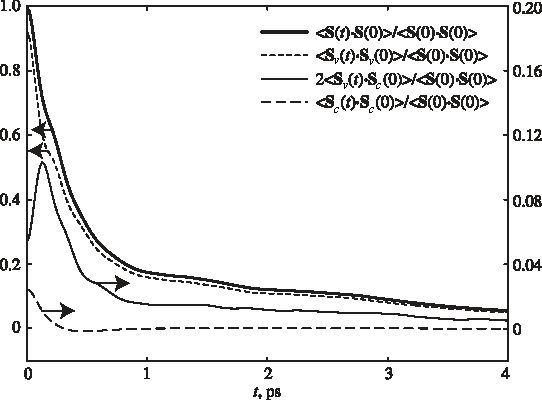
\includegraphics[width=8cm]{chapters/chapter2/figures/McGaughey-argon-contributions.pdf}
    \caption{Breakdown of the energy flux autocorrelation function $\langle\mathbf{J}^\smallE(t)\cdot\mathbf{J}^\smallE(t)\rangle$ of LJ fcc solid argon at $50\un{K}$ into the three terms of Eq.~\eqref{eq:JtJ0-components}. Note that the total ACF and the virial component correspond to the left vertical axis, while the cross and convection curves correspond to the right axis. Reproduced from Ref.~\cite{McGaughey2006}.}
    \label{fig:argon-convective}
\end{figure}

The first term on the right-hand side of Eq.~\eqref{eq:J-classical},
\begin{equation}
    \mathbf{J}^\smallE_c = \frac{1}{\rOmega} \sum_n \mathbf{V}_n e_n , \label{eq:J-convective}
\end{equation}
is often called \emph{convective} (or \emph{kinetic}) and the second term,
\begin{equation}
    \mathbf{J}^\smallE_v = \frac{1}{\rOmega} \left[ \sum_{n,m} (\mathbf{R}_n-\mathbf{R}_m) \mathbf{F}_{n m} \cdot \mathbf{V}_n \right], \label{eq:J-virial}
\end{equation}
is often called \emph{virial} (or \emph{potential}).
\citet{Fan2015} and \citet{Carbogno:2017gc}, for example, adopt this nomenclature and state that the convective term $\mathbf{J}^\smallE_c$ ``\emph{gives no contributions to the conductivity tensor in solids, as mass transport is negligible}''.
We feel that the wording ``convective'' is somewhat misleading in this context, as the contribution of the convective current $\mathbf{J}^\smallE_c$ to the heat conductivity may not vanish even in the absence of convection, especially in softer solid materials. 
Using Eqs.~\eqref{eq:J-convective} and \eqref{eq:J-virial}, the energy flux autocorrelation function can be split into 3 terms:
\begin{equation}
    \langle\mathbf{J}^\smallE(t)\cdot\mathbf{J}^\smallE(t)\rangle = \langle\mathbf{J}_c^\smallE(t)\cdot\mathbf{J}_c^\smallE(t)\rangle + 
    2\langle\mathbf{J}_c^\smallE(t)\cdot\mathbf{J}_v^\smallE(t)\rangle + 
    \langle\mathbf{J}_v^\smallE(t)\cdot\mathbf{J}_v^\smallE(t)\rangle . \label{eq:JtJ0-components}
\end{equation}
Their contributions to thermal conductivity were computed by \citet{McGaughey2006} for a LJ fcc argon crystal at $50\un{K}$ (the breakdown of $\langle\mathbf{J}^\smallE(t)\cdot\mathbf{J}^\smallE(t)\rangle$ into the three terms of Eq.~\eqref{eq:JtJ0-components} is shown in Fig.~\ref{fig:argon-convective}). They found that while the convection contribution $\langle\mathbf{J}_c^\smallE(t)\cdot\mathbf{J}_c^\smallE(t)\rangle$ was indeed small ($\sim 1\%$), the contribution of the cross term $2\langle\mathbf{J}_c^\smallE(t)\cdot\mathbf{J}_v^\smallE(t)\rangle$ is not insignificant ($\sim 10\%$). 
The relative contributions of the convective and cross terms increase as the temperature goes up and anharmonic effects inhibit ``pure'' conduction. 
The absolute values of the convective contribution remains the same with increasing temperature, whereas the virial and cross term contributions decrease. \LEnote{<-- check this**}
While the convective term may not be as important for materials with higher thermal conductivity, in general, its contribution and that of the cross term should be checked before assuming they are negligible. Some further comments on this issue in Sec.~\ref{sec:carbogno}. 

In the literature the nomenclature is often confusing, and the relative contributions of each term is often not very well known. 
For example, \citet{Vogelsang1987} divide the energy currents in two terms \cite{McQuarrie2000}: a ``\emph{kinetic}'' part, defined as
\begin{equation}
    {\mathbf{J}^\smallE_k}' = \frac{1}{\rOmega} \frac{(\mathbf{P}_n)^2}{2M_n} \mathbf{V}_n ,
\end{equation}
and a ``\emph{potential}'' part, defined as
\begin{equation}
    {\mathbf{J}^\smallE_p}' = \frac{1}{\rOmega} \left[ \sum_n  v_n(\{\mathbf{R}\}) \mathbf{V}_n + \sum_{n,m} (\mathbf{R}_n-\mathbf{R}_m) \mathbf{F}_{n m} \cdot \mathbf{V}_n \right] .
\end{equation}
They find that ${\mathbf{J}^\smallE_k}'$ is negligible in solids, where atomic diffusion does not occur.
\citet{Kinaci2012}, instead, use the Einstein formulation and define a ``\emph{kinetic}'' term
\begin{equation}
    {\mathbf{J}^\smallE_k}'' = \frac{1}{\rOmega} \left[ \frac{(\mathbf{P}_n)^2}{2M_n} \mathbf{V}_n + \sum_{n,m} (\mathbf{R}_n-\mathbf{R}_m) \mathbf{F}_{n m} \cdot \mathbf{V}_n \right],
\end{equation}
and a ``\emph{potential}'' term
\begin{equation}
    {\mathbf{J}^\smallE_p}'' = \frac{1}{\rOmega} \sum_n  v_n(\{\mathbf{R}\}) \mathbf{V}_n ,
\end{equation}
and conclude that in perfect solid systems, where diffusion is highly improbable, ${\mathbf{J}^\smallE_p}''$ contribution to thermal conductivity is negligible.

Finally, an alternative definition of the heat current can be used when dealing with solids \cite{Ladd1986}:
\begin{equation}
    \mathbf{J}^\smallE(\rGamma) =
       \frac{1}{\rOmega} \sum_{n,m} (\mathbf{R}_n^0 -\mathbf{R}_m^0) \mathbf{F}_{n m} \cdot \mathbf{V}_n , \label{eq:J-leyla}
\end{equation}
where $\mathbf{R}_n^0$ denotes the average atomic position of atom $n$. One should not confuse this expression with neglecting the convection part of the heat current. For a solid, Eq.~\eqref{eq:J-leyla} will give the same thermal conductivity as Eq.~\eqref{eq:J-classical-2body}, as demonstrated in Sec.~\ref{sec:carbogno}.


\paragraph{Many-body potentials}
In the case of a many-body potential interaction, if the atomic potential energy can be written as a function of the distance vectors $\mathbf{R}_{nm}=\mathbf{R}_n-\mathbf{R}_m$, as $v_n = v_n(\mathbf{R}_{1n},\mathbf{R}_{2n},\cdots,\mathbf{R}_{Nn})$, the force acting on atom $n$ can be written as \cite{Fan2015,Hardy2016}:
\begin{align}
    \mathbf{F}_n &= -\sum_m \frac{\partial v_m}{\partial \mathbf{R}_n} = \sum_m \sum_{p\neq n} \frac{\partial v_m}{\partial \mathbf{R}_{pn}} \nonumber\\
        &= \sum_m \sum_{p\neq n} \left(\frac{\partial v_m}{\partial \mathbf{R}_{mn}} \delta_{pm} + \frac{\partial v_m}{\partial \mathbf{R}_{pn}} \delta_{mn} \right) \nonumber\\
        &= -\sum_{m\neq n} \left( \frac{\partial v_n}{\partial \mathbf{R}_{nm}} - \frac{\partial v_m}{\partial \mathbf{R}_{mn}} \right).
\end{align}
For example, for the Tersoff \cite{Tersoff1989} and Swillinger-Weber \cite{Stillinger1985} potentials, \citet{Fan2015} obtain the following definition for the virial energy flux:
\begin{equation}
    \mathbf{J}^\smallE_v = \sum_n \sum_{n\neq m} \mathbf{R}_{nm} \left(\frac{\partial v_m}{\partial \mathbf{R}_{mn}} \cdot \mathbf{V}_n \right) ,
\end{equation}
equivalent to the one obtained by \citet{Hardy1963}, and they show that other two-body like formulations widely reported in the literature may give wrong results, especially in low-dimensional systems.

\end{LEtext}


\subsection{Multi-component fluids} \label{sec:multi-component}
In a multi-component fluid there is one conserved quantity (the particle number) per atomic species, plus the total energy and the three Cartesian components of the total momentum. The momentum densities are mass currents: the mass flux is therefore the total momentum, which vanishes in the center of mass reference frame. The transverse components of the momentum densities are decoupled from the other conserved densities \cite{Foster1975}, while the longitudinal one can be assumed to coincide with the total momentum in the long-wavelength limit. Momentum conservation thus constrains the number of fluxes interacting with the energy flux in Eq.~\eqref{eq:onsager} to $Q-1$, $Q$ being the number of atomic species, so that the resulting dimension of the matrix of Onsager coefficients, $L$, is $Q\times Q$. The heat flux is defined as the non-convective component of the energy flux, \emph{i.e.} the value of the latter in the absence of mass transport, that is to say when all the particle fluxes vanish.\footnote{It is unfortunate, but inevitable due to common usage, that this definition of non-convective flux clashes with a different definition given above while dividing Eq.~\eqref{eq:J-classical-2body} into two terms.} By imposing this condition in Eq.~\eqref{eq:onsager}, with $\mathbf J^\smallone \equiv \mathbf{J}^\smallE$, and $\mathbf{J}^{q}$ ($q =2,\dots Q$) being independent particle fluxes, the thermal conductivity, defined by the Fourier's law as the ratio of the heat flux over the temperature gradient, is given by:
\begin{equation}
\kappa = \frac{1}{T^2 \,(L^{-1})^{\smallone\smallone}}. \label{eq:multi_kappa}
\end{equation}
This expression can be proved to be invariant under \textit{any} non-singular linear transformation of the independent particle fluxes. 

\paragraph{Two-component fluids}
For instance, in the case of a two-component liquid, energy and particle currents are coupled as in:
\begin{equation}
  \begin{aligned}
    \mathbf{J}^\smallE &= L^{\smallE\smallE}\,  \nabla \left (\frac{1}{T} \right ) + L^{\smallE\smallQ} \, \nabla \left (\frac{\mu}{T} \right ), \\
    \mathbf{J}^{\smallQ} &= L^{\smallE\smallQ} \, \nabla \left (\frac{1}{T} \right ) + L^{\smallQ\smallQ} \, \nabla \left (\frac{\mu}{T} \right ), \label{eq:two-comp-constitutive}
  \end{aligned}
\end{equation}
where $\mathbf{J}^{\smallQ}$ is the particle current of one of the two species (say, the second), and $\mu$ the corresponding chemical potential \cite{Sindzingre1990}. By imposing that the particle current vanishes, the resulting thermal conductivity is:
\begin{equation}
  \kappa=\frac{1}{T^2}
  \left( L^{\smallE\smallE} - \frac{(L^{\smallE\smallQ})^2}{L^{\smallQ\smallQ}} \right). \label{eq:two-comp-kappa}
\end{equation}


\bigskip
\bigskip
\LEnote{***** QUANTUM EFFECTS ??? *****}
  % Green-Kubo
\chapter{Gauge invariance of heat transport coefficients} \label{ch:gauge-invariance}

It is often implicitly assumed that the well-definiteness of thermal transport coefficients would stem from the uniqueness of the decomposition of the system's total energy into localized, atomic, contributions. This assumption is manifestly incorrect, as any decomposition leading to the same value for the total energy as Eq.~\eqref{eq:atomic-energies} should be considered as legitimate. The difficulty of partitioning a system's energy into subsystems' contributions is illustrated in Fig.~\ref{fig:energy-partition}, which depicts a system made of two interacting subsystems. When defining the energy of each of the two subsystems, an arbitrary decision has to be made as to how the interaction energy is partitioned. In the case depicted in Fig.~\ref{fig:energy-partition}, for instance, the energy of each of the two subsystems can be defined as $\mathcal{E}(\rOmega_i) = E(\rOmega_i) + \frac{1}{2}(1\pm\lambda)W_{12}$, where $E(\rOmega_i)$ are the energies of the two isolated subsystems, $W_{12}$ their interaction energy, and $\lambda$ an arbitrary constant. In the thermodynamic limit, when all the subsystems' energies are much larger than the interaction between any pairs of them, the value of the $\lambda$ constant is irrelevant. When it comes to defining energy densities (\emph{i.e.} energies of infinitesimal portions of a system) or atomic energies, instead, the magnitude of the interaction between different subsystems is comparable to their energies, which become therefore intrinsically ill-defined.

\begin{figure}
\begin{minipage}{0.5\textwidth}
\centering 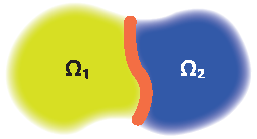
\includegraphics{chapters/chapter3/figures/blob.pdf}
\end{minipage}
\begin{minipage}{0.4\textwidth}
\begin{align*}
  E(\rOmega_{1}\cup\rOmega_2) &= E(\rOmega_1) + E(\rOmega_2) + W_{12} \qquad \\
  & \overset{?}{=}\mathcal{E}(\rOmega_1)+\mathcal{E}(\rOmega_2)
\end{align*}
\end{minipage}
\caption{
	The energy of an isolated system is the sum of the energies of its subsystems (as defined when they are isolated as well) plus the interaction among them, $W_{12}$, whose magnitude scales as the area of the interface, depicted in red. When defining the energies of individual subsystems, $\mathcal{E}$, $W_{12}$ has to be arbitrarily partitioned among them. \label{fig:energy-partition}}
\end{figure}

Let us consider a mono-atomic fluid interacting through pair potentials, $v(|\mathbf{R}_n-\mathbf{R}_m|)$, and define the atomic energies as \citep{Marcolongo2014,Ercole2016}:
\begin{equation}
  e_{\smallgamma,n}(\rGamma) =
  \frac{1}{2M_n}(\mathbf{P}_{n})^{2} + \frac{1}{2}\sum_{m\ne n}
  v(|\mathbf{R}_{n}-\mathbf{R}_{m}|)
  (1+\gamma_{nm}), \label{eq:Lambda-atomic-energies}
\end{equation}
where $\gamma_{nm}=-\gamma_{mn}$ is \emph{any} antisymmetric matrix.
As the inter-atomic potential appearing in Eq.~\eqref{eq:Lambda-atomic-energies} is symmetric with respect to the atomic indices, it is clear that the sum of all the atomic energies does not depend on $\gamma$, thus making any choice of $\gamma$ equally permissible. This trivial observation has deep consequences on the theory of thermal fluctuations and transport, because the value of the macroscopic energy flux, instead, depends explicitly on $\gamma$, thus making one fear that the resulting transport coefficients would depend on $\gamma$ as well. Using the same manipulations that lead from Eqs.~\eqref{eq:epsilon-classical} and \eqref{eq:atomic-energies} to Eq.~\eqref{eq:J-classical}, for any choice of the $\gamma$ matrix in Eq.~\eqref{eq:Lambda-atomic-energies}, a corresponding expression for the macroscopic energy flux can be found, reading \citep{Marcolongo2014,Ercole2016}:
\begin{equation}
  \mathbf{J}_{\smallgamma}^\smallE=\mathbf{J}^\smallE+
  \frac{1}{2 \rOmega}\sum_{n,m\ne n}\gamma_{nm} \Bigl ( v_{nm} \mathbf{V}_{n} + \bigl (\mathbf{V}_{n}\cdot \nabla_{\mathbf{R}_n} v_{nm} \bigr )  (\mathbf{R}_{n}-\mathbf{R}_{m}) \Bigr ), \label{eq:Lambda-classical-current}
\end{equation}
where $v_{nm}= v(|\mathbf{R}_{n} - \mathbf{R}_{m}|)$.

\begin{figure}
    \begin{center}
        \subfigure[\label{fig:argon-gauge-acf}]{\includegraphics[width=10cm]{chapters/chapter3/figures/handbook_argon_egauge_acf.pdf}}
        \subfigure[\label{fig:argon-gauge-kappa}]{\includegraphics[width=10cm]{chapters/chapter3/figures/handbook_argon_egauge_kappa.pdf}}
    \end{center}
	\caption{(a) Time correlation functions of the modified macroscopic energy flux of a Lennard-Jones fluid, at the conditions described in the text, as defined in Eq.~\eqref{eq:Lambda-classical-current}, for different definitions of the $\gamma$ matrix. The ``0'' line refers to the standard definition ($\gamma = 0$), whereas the labels ``1'' and ``2'' correspond to two other (arbitrary) definitions of $\gamma$ as described in \cite{Ercole2016}.
    (b) Integral of the time correlation functions displayed in Fig.~\ref{fig:argon-gauge-acf}, multiplied by the prefactor appearing in the GK relation, Eq.~\eqref{eq:GK-complete}, as a function of the upper limit of integration. The barely visible shaded area surrounding each line is an indication of the error bars, as estimated by standard block analysis. Units are Lennard-Jones units ($M=\sigma=\varepsilon=1$). \label{fig:argon-gauge}}
\end{figure}

As a specific example, \cite{Ercole2016} ran MD simulations for a Lennard-Jones monoatomic fluid described by the inter-atomic potential $v(r)=\epsilon \left [ \left ( \frac{\sigma}{r}\right )^{12} - \left ( \frac{\sigma}{r}\right )^{6}\right ] $ at temperature $T=1.86 \frac{\epsilon}{k_B}$ and density $\rho=0.925 \sigma^{-3}$. In Fig.~\ref{fig:argon-gauge-acf} we display the resulting macroscopic energy-flux autocorrelation function corresponding to different choices of the $\gamma$ matrix in Eqs.~\eqref{eq:Lambda-atomic-energies} and \eqref{eq:Lambda-classical-current}. Fig.~\ref{fig:argon-gauge-acf} clearly shows that the $\langle \mathbf{J}^\smallE_{\gamma}(t) \cdot\mathbf{J}^\smallE_{\gamma}(0) \rangle$ correlation functions dramatically depend on the $\gamma$ matrices in Eqs.~\eqref{eq:Lambda-atomic-energies} and \eqref{eq:Lambda-classical-current}.  Notwithstanding, the integrals of all these time correlation functions tend to the same limit at large integration times, as shown in Fig.~\ref{fig:argon-gauge-kappa}.

In order to get insight into this remarkable invariance property, let us inspect the difference between the generalized flux in Eq.~\eqref{eq:Lambda-classical-current} and the standard expression of Eq.~\eqref{eq:J-classical}:
\begin{equation}
  \rDelta\mathbf{J}^\smallE_{\smallgamma} =\mathbf{J}^\smallE_{\smallgamma}-\mathbf{J}^\smallE  =\frac{\mathrm{d}}{\mathrm{dt}}\frac{1}{4 \rOmega} \sum_{n,m\ne n}  \gamma_{nm} \, v(|\mathbf{R}_{n}-\mathbf{R}_{m}|)  (\mathbf{R}_{n}-\mathbf{R}_{m}). \label{eq:DeltaJ}
\end{equation}
We see that the two different expressions for the macroscopic energy flux differ by a total time derivative of a bounded phase-space vector function. In the following, we show that this is a consequence of energy conservation and extensivity and a sufficient condition for the corresponding thermal conductivities to coincide.

The very possibility of defining an energy current density, from which the energy fluxes of Eq.~\eqref{eq:J-classical} and \eqref{eq:Lambda-classical-current} ultimately depend, stems from energy extensivity. The considerations illustrated in Fig.~\ref{fig:energy-partition} indicate that any two densities, $e'(\mathbf{r},t)$ and $e(\mathbf{r},t)$, whose integrals over a macroscopic volume differ by a quantity that scales as the volume boundary, should be considered as equivalent. This equivalence can be expressed by the condition that two equivalent densities differ by the divergence of a (bounded) vector field:
\begin{equation}
  e'(\mathbf{r},t)=e(\mathbf{r},t) - \nabla\cdot \bm{p}(\mathbf{r},t). \label{eq:gauge_transformation}
\end{equation}
In a sense, two equivalent energy densities can be thought of as different \emph{gauges} of the same scalar field. Energy is also conserved: because of this, for any given gauge of the energy density, $e(\mathbf{r},t)$, an energy current density can be defined, $\bm{j}(\mathbf{r},t)$, so as to satisfy the continuity equation, Eq.~\eqref{eq:continuity}. By combining Eqs.~\eqref{eq:gauge_transformation} and \eqref{eq:continuity} we see that energy current densities and macroscopic fluxes transform under a gauge transformation as:
\begin{align}
 \bm{j}'(\mathbf{r},t) & = \bm{j}(\mathbf{r},t) + \dot{\bm{p}}(\mathbf{r},t), \label{eq:current_density_gauge} \\
  \mathbf{J}'(t) & = \mathbf{J}(t) + \dot{\mathbf{P}}(t), \label{eq:macroscopic_flux_gauge}
\end{align}
where $\mathbf{P}(t)=\frac{1}{\rOmega} \int\bm{p}(\mathbf{r},t)d\mathbf{r}$. We
conclude that the macroscopic energy fluxes in two different energy gauges differ by the total time derivative of a bounded phase-space vector function.

We now show that the energy fluxes of the same system in two different energy gauges, $e$ and $e'$, differing by a bounded total time derivative, as in Eq.~\eqref{eq:macroscopic_flux_gauge}, result in the same heat conductivity, as given by the Green-Kubo formula, Eq.~\eqref{eq:GK-complete}. More generally, the Onsager coefficients coupling two fluxes, $\mathbf{J}^1$ and $\mathbf{J}^2$, do not depend on the gauge of either one of them. In fact, let $\left(\mathbf{J}^1\right)' = \mathbf{J}^1 + \dot{\mathbf{P}}$; one has:
\begin{equation}
  \begin{aligned}
    \left (L^{11} \right)' &= \frac{\rOmega}{2 k_B }\int_{-\infty}^{+\infty} \left \langle \left (\mathbf{J}_1(t)+\dot{\mathbf{P}}(t) \right ) \cdot  \left (\mathbf{J}_1(0)+\dot{\mathbf{P}}(0)\right ) \right \rangle dt \\
    &= L^{11} + \frac{\rOmega}{2 k_B } \left[ \left .  \left \langle \mathbf{P}(t) \cdot \dot{\mathbf{P}}(0) \right \rangle \right |^{+\infty}_{-\infty} + \left .  2 \Bigl \langle \mathbf{P}(t) \cdot \mathbf{J}_1(0) \Bigr \rangle \right |^{+\infty}_{-\infty} \right] .
  \end{aligned} \label{eq:L=L'}
\end{equation}

The expectation of the time-lagged products in Eq.~\eqref{eq:L=L'} is equal to the products of two expectations at large time lag. As the equilibrium expectations of both a total time derivative and a current vanish, we conclude that $\left (L^{11}\right )'=L^{11}$. A slight generalization of this argument, also using microscopic reversibility as in \cite{Onsager1931a,Onsager1931b}, allows us to conclude that $\left (L^{12} \right )'=L^{12}$ and that, in general, $\kappa'=\kappa$.


\section{Molecular fluids} \label{sec:MolecularFluids}
In a one-component molecular fluid such as liquid water or, say, ethanol, there are in general $Q$ fluxes interacting with each other through Onsagers' Eq.~\eqref{eq:onsager}, where $Q$ is the number of atomic species in a molecule. The requirement that atoms are bound in molecules of fixed composition, however, sets a number of constraints that substantially simplify the treatment of heat transport, making the molecular case similar to the one-component one.

Let us consider a molecule of chemical formula $A_{N_A} B_{N_B}\cdots$, where $A, B,\cdots$ indicate atomic species, and $N_A,N_B,\cdots$ the corresponding atomic stoichiometric indices. For each atomic species we define the normalized number flux as:
\begin{equation}
  \mathbf{J}^X = \frac{1}{N_X}\sum_{n\in X} \mathbf{V}_n. \label{eq:JX}
\end{equation}
If we indicate by $M_X$ the atomic mass of species $X$, momentum conservation requires that $\sum_X M_X N_X \mathbf{J}^X = 0$ in the center-of-mass reference frame. The flux $\mathbf{J}^{XY} = \mathbf{J}^{X}-\mathbf{J}^{Y}$ is the total time derivative of a bounded vector, because its integral is the sum over all the molecules of the difference between the average atomic positions of either species within a same molecule, which is obviously bounded if molecules do not dissociate. As any number flux $\mathbf{J}^X$ can be expressed as a linear combination of the total momentum and of several $\mathbf{J}^{XY}$ fluxes, each of them is the total time derivative of a bounded vector. Therefore, the Onsager coefficient coupling any of these atomic fluxes with any other, or with the energy flux, vanishes. We conclude that energy is the only conserved quantity relevant for heat transport in a molecular fluid, and that the energy-flux autocorrelation function directly yields the thermal conductivity, as in Eq.~\eqref{eq:GK}.

  % Gauge invariance
\chapter{Density-functional theory of adiabatic heat transport} \label{ch:dft-heat}

\begin{LEtext}
The advent of density-functional theory (DFT) \cite{Hohenberg1964,Kohn1965} has marked the start of a new era for the quantum modeling of materials. DFT allows computing interatomic forces entirely from first principles using the chemical composition and the fundamental laws of nature as the sole ingredients, without any need to leverage experimental knowledge of these interactions.
Its combination with classical molecular dynamics, both in the Born-Oppenheimer of Car-Parrinello flavours \cite{Car1985,Marx2009}, had a groundbreaking impact in a wide number of physical problems.

Nevertheless, quantum simulation methods based on DFT have long been thought to be incompatible with the GK theory of thermal transport \emph{because in first-principles calculations it is impossible to uniquely decompose the total energy into individual contributions from each atom}. \citep{Stackhouse2010b} For this reason, \emph{ab initio} simulations of heat transport have often been performed using non-equilibrium approaches.

The recently discovered gauge invariance principle that was introduced in Chapter~\ref{ch:gauge-invariance} not only explains why an arbitrary defintion of the heat flux results in a well-defined value for the thermal conductivity, but it also gives a rigorous way of deriving an expression for the energy flux directly from DFT, without introducing any \emph{ad hoc} ingredients.

In this chapter we first summarize the most recent \emph{ab initio} methods for the computation of thermal conductivity. Then we briefly review the first-principles GK theory of thermal transport developed by \citet{Marcolongo2014}, that will be adopted in the rest of this work.
\end{LEtext}


\section{First-principles simulation methods}

In insulators heat transport is determined by the dissipative dynamics of atoms, the electrons following adiabatically in their ground state, a regime often referred to as atomic or \emph{adiabatic heat conduction}. Different approaches are available to model heat conduction in these systems: the main ones are the \emph{Boltzmann's transport equation} (BTE), \emph{non-equilibrium Green's functions} (NEGF), and \emph{molecular dynamics} (MD), both in its non-equilibrium and equilibrium flavors. 

\emph{Non-equilibrium Green's functions} (NEGF) \cite{Wang2008} are designed to compute the conductance of open systems, such as nanoscale devices and interfaces, but they do not apply to bulk conduction. 

The \emph{Boltzmann's transport equation} (BTE) \cite{Peierls1929,Zhou2016} is the method of choice for crystals well below melting, where long-lived phonons are clearly identified as the heat carriers. In this case density-functional perturbation theory \cite{Baroni1987a,Gonze1989,Baroni2001} allows one to compute accurate phonon frequencies \cite{Giannozzi1991} and lifetimes, \cite{Debernardi1995,Paulatto2013} and thus implement the BTE entirely from first principles. \cite{Broido:2007iu} 
The flexibility and accuracy of \abinitio BTE are such that this approach is being successfully used to screen new materials for custom-designed properties, such as high thermal conductivity for passive cooling \cite{Lindsay:2013fw,Lindsay:2013db} or low thermal conductivity for thermoelectric energy conversion. \cite{PhysRevX.4.011019,Schwingen2014} 
Recent self-consistent and variational approaches to solve the BTE beyond the relaxation-time approximation \cite{Fugallo2013} are also providing fresh and deep insight into the collective character of heat transport.\cite{Fugallo2013,Lee:2015ex,Cepellotti2015,Cepellotti:2016bk} 
Yet, the applicability of \emph{ab initio} BTE is restricted to periodic systems consisting of a small number of atoms per unit cell, and is severely limited by its own inherent approximations: as the temperature increases, anharmonic effects become so important as to eventually make it break down well below melting, \cite{Turney:2009bb} while the BTE simply does not apply to glasses and liquids, where phonons are not even defined. \cite{Allen1989} 

\emph{Molecular dynamics} (MD) \cite{Allen1989,Frenkel2001} is set to overcome these limitations. 
In non-equilibrium MD (NEMD), \cite{Evans1990,Muller-Plathe1997} temperature gradients or heat fluxes are explicitly imposed on the virtual sample, and the thermal conductivity is estimated from the resulting value of the conjugate variable (flux or gradient). 
In the so-called \emph{approach to equilibrium} (AEMD) methodology of \citet{Lampin2013} the system is first prepared in an out-of-equilibrium state, characterized by an inhomogeneous temperature distribution, and the thermal conductivity is evaluated from the time it takes for the system to equilibrate. 
NEMD and AEMD lend themselves to a straightforward quantum-mechanical implementation \cite{Stackhouse2010b,Bouzid2017} using \emph{ab initio} molecular dynamics (AIMD). For example, \citet{Stackhouse2010b} computed the thermal conductivity of periclase MgO using a method devised by \citet{Müller-Plathe1997}, \emph{i.e.} by imposing a temperature gradient to the system, and evaluating the ratio between the heat flux and the resulting temperature gradient.
\citet{Bouzid2017} combined AEMD with AIMD to simulate thermal transport in a GeTe$_4$ glass, while \citet{Puligheddu2017} further generalized and applied it to crystalline and nano-structured MgO.
However, but methods may be both affected by non-linear effects, due to the strength of the temperature gradient to be imposed \cite{Schelling2002,He2012} and by finite-size/finite-time effects that require long simulation times and difficult extrapolations to approach the thermodynamic limit. \cite{sellan2010,He2011,He2012,Zaoui2016,Wang2017}

The combination of equilibrium molecular dynamics (EMD), based on the Green-Kubo theory, with DFT, has been successfully accomplished very recently by \citep{Marcolongo2016}, thanks to the gauge-invariance principle introduced in Chapter~\ref{ch:gauge-invariance}, that gives a rigorous way of deriving an expression for the energy flux directly from DFT, without introducing any \emph{ad hoc} ingredients. We describe this approach in Sec.~\ref{sec:dft-heat-theory} and we will use it in the rest of this work. (***RIFERIMENTI***)

More recently, several works attempted to combine the GK approach to heat transport with first-principles techniques based on electronic-structure theory, by adopting some \emph{ad hoc} definitions for the energy flux. \citet{Kang2017}, for instance, derived an expression for the energy flux from a (rather arbitrary) quantum-mechanical definition of the atomic energies and used a modified MD integration algorithm to cope with the difficulties ensuing from the implementation of their expression in PBC. 
\citet{Carbogno:2017gc} gave a different expression for the energy flux, that neglects the convective term (**EQ.**) and is based on a normal-mode decomposition of the atomic coordinates and forces, which, while allowing to reduce the effects of thermal fluctuations, can only be applied to crystalline solids.

\citet{English2017}, instead, used the classical Einstein relation for the energy displacement, $\mathcal{D}(\tau) = \sum_n \mathbf{R}_n \int_0^\tau \mathbf{F}_n \cdot \mathbf{V}_n \, dt$, computed from a BO-AIMD trajectory, where the forces are computed from the Hellmann-Feynman theorem. They applied this methodology to the computation of thermal conductivity of periclase MgO \cite{Tse2018} and other solids. Their approach also neglects the convective term and is only applicable to solids.


\section{DFT heat flux}  \label{sec:dft-heat-theory}
The gauge invariance principle presented in Chapter~\ref{ch:gauge-invariance} provides a rigorous way to derive an expression for the adiabatic energy flux from DFT.
In order to derive such an expression, we start with the standard DFT expression of the total energy in terms of the Kohn-Sham (KS) eigenvalues $\varepsilon_v$, eigenfunctions $\phi_v(\mathbf{r})$, and density $n(\mathbf{r}) = \sum_v |\phi_v(\mathbf{r})|^2$ \citep{Martin2008}:
\begin{multline}
  E_{\smallDFT} = \frac{1}{2}\sum_{n}M_{n}V_{n}^{2} + \frac{\mathtt{e}^2}{2}\sum_{n,m\ne n}\frac{ Z_{n}Z_{m}}{|\mathbf{R}_{n}-\mathbf{R}_{m}|} \\
  + \sum_{v}\varepsilon_{v}-\frac{\mathtt{e}^2}{2}\int\frac{n(\mathbf{r})n(\mathbf{r}')}{|\mathbf{r}-\mathbf{r}'|}d\mathbf{r}d\mathbf{r}'+\int\left(\epsilon_{\smallXC}[n](\mathbf{r})-\mu_{\smallXC}[n](\mathbf{r})\right)n(\mathbf{r})d\mathbf{r},
\end{multline}
where $\mathtt{e}$ is the electron charge, $\epsilon_\smallXC[n](\mathbf{r})$ is a local exchange-correlation (XC) energy per particle defined by the relation $ \int \epsilon_\smallXC[n](\mathbf{r})n(\mathbf{r}) d\mathbf{r}=E_\smallXC [n]$, the latter being the total XC energy of the system, and $ \mu_\smallXC (\mathbf{r}) = \frac{\delta E_\smallXC }{\delta n(\mathbf{r})}$ is the XC potential. The DFT total energy can be readily written as the integral of a DFT energy density \citep{Chetty1992}:
\begin{equation}
  \begin{aligned}
    E_{\smallDFT} & =  \int e_{\smallDFT}(\mathbf{r})d\mathbf{r},\\
    e_{\smallDFT}(\mathbf{r}) & = e_{el}(\mathbf{r})+e_{\smallZ}(\mathbf{r}),
  \end{aligned}
  \label{eq:DFT-Edensity}
\end{equation}
where:
\begin{align}
  e_{el}(\mathbf{r}) & =\mathfrak{Re} \sum_{v}\phi_{v}^{*}(\mathbf{r})\bigl(H_{\smallKS}\phi_{n}(\mathbf{r})\bigr) \nonumber \\
  & \qquad\qquad\qquad - \frac{1}{2}n(\mathbf{r})v_{\smallH}(\mathbf{r}) +\left(\epsilon_\smallXC (\mathbf{r}) - \mu_\smallXC  (\mathbf{r}) \right) n(\mathbf{r}), \\
  e_{\smallZ}(\mathbf{r}) & = \sum_{n}\delta(\mathbf{r}-\mathbf{R}_{n}) \left(\frac{1}{2}M_{n}V_{n}^{2}+w_{n}\right), \\
  w_{n} & =\frac{\mathtt{e}^2}{2}\sum_{m\ne n}\frac{ Z_{n}Z_{m}}{|\mathbf{R}_{n}-\mathbf{R}_{m}|}, \label{eq:DFT-Edensity-breakup}
\end{align}
$H_\smallKS$ is the instantaneous self-consistent Kohn-Sham Hamiltonian, and $v_\smallH = \mathtt{e}^2 \int d\mathbf{r}' \frac{n(\mathbf{r}')}{|\mathbf{r}-\mathbf{r}'|}$ is the Hartree potential. An explicit expression for the DFT energy flux is obtained by computing the first moment of the time derivative of the energy density, Eqs.~(\ref{eq:DFT-Edensity}-\ref{eq:DFT-Edensity-breakup}), as indicated in Eq.~\eqref{eq:JE=rdote}, resulting in a number of terms, some of which are either infinite or ill-defined in PBC. Casting the result in a regular, boundary-insensitive, expression requires a careful breakup and refactoring of the various harmful terms, as explained by \cite{Marcolongo2014} and in the online version of \cite{Marcolongo2016}. The final result reads:
\begin{align}
  \allowdisplaybreaks
  \mathbf{J}^\smallE_{\smallDFT} &=\mathbf{J}^{\smallH} + \mathbf{J}^{\smallZ} + \mathbf{J}^{0} + \mathbf{J}^{\smallKS} +  \mathbf{J}^{\smallXC}, \\
  \mathbf{J}^{\smallH} &=
  \frac{1}{4\pi \rOmega \mathtt{e}^2}\int \nabla v_{\smallH}(\mathbf r) \dot v_{\smallH}(\mathbf  r) d\mathbf{r}, \\
  \mathbf{J}^{\smallZ} \label{eq:DFT-ionic} &=
  \frac{1}{\rOmega} \sum_{n}  \left[\mathbf{V}_{n}\left(\frac{1}{2}M_{n}V_{n}^{2} + w_{n}\right) + \sum_{m\ne n}(\mathbf{R}_{n} - \mathbf{R}_{m}) \left(\mathbf{V}_{m} \cdot \frac {\partial w_{n}}{\partial \mathbf{R}_{m}} \right) \right], \\
  \mathbf{J}^{0}  &=
  \frac{1}{\rOmega}  \sum_{n} \sum_{v}\left\langle \phi_{v} \left|(\mathbf{r}-\mathbf{R}_{n})\left(\mathbf{V}_{n}\cdot\frac{\partial\hat{v}_{0}}{\partial\mathbf{R}_{n}}\right)\right| \phi_{v}\right\rangle, \\
  \mathbf{J}^{\smallKS} &= \label{eq:DFT-KS}
  \frac{1}{\rOmega}  \mathfrak{Re} \sum_{v} \langle \bm{\bar \phi}_v^c | H_{\smallKS}+\varepsilon_v | \dot \phi_v^c \rangle, \\
  J_\alpha^{\smallXC} &=
  \begin{cases}
    0 & \mathrm{(LDA)} \\
      -\frac{1}{\rOmega} \int n(\mathbf{r}) \dot{n}(\mathbf{r}) \frac{\partial\epsilon^{\smallGGA} (\mathbf{r})}{\partial(\partial_\alpha n)} d\mathbf{r} & \mathrm{(GGA)},
  \end{cases}
\end{align}
where  $\hat v_0$ is the bare, possibly non-local, (pseudo-) potential acting on the electrons and
\begin{align}
  |\bm{\bar \phi}_v^c\rangle &= \hat P_c \,\mathbf{r}  \,|\phi_v \rangle, \label{eq:r-times-phi} \\
  |\dot \phi_v^c\rangle &= \dot{\hat P}_v \,|\phi_v\rangle, \label{eq:phi-dot}
\end{align}
are the projections over the empty-state manifold of the action of the position operator over the $v$-th occupied orbital, Eq.~\eqref{eq:r-times-phi}, and of its adiabatic time derivative \citep{Giannozzi2017}, Eq.~ \eqref{eq:phi-dot}, $\hat P_v$ and $\hat P_c = 1 - \hat P_v$ being the projector operators over the occupied- and empty-states manifolds, respectively. Both these functions are well defined in PBC and can be computed, explicitly or implicitly, using standard density-functional perturbation theory \citep{Baroni2001}.
  % DFT heat transport
\chapter{Estimation of heat transport coefficients}  \label{ch:data-analysis}

The evaluation of transport coefficients in extended systems, such as thermal conductivity or shear viscosity, is known to require impractically long simulations. The Green-Kubo equation, Eq.~\eqref{eq:GK-complete}, expresses the thermal conductivity as the integral of the autocorrelation function of the heat flux, \emph{i.e.} an autocorrelation time. 

Many methods have been formulated to estimate its value from finite-length MD simulations: direct time-integration methods, fitting with exponential functions, and spectral methods; however, few of them provide a rigorous criterion to estimate the accuracy resulting from a given MD trajectory. Different classes of systems require different approaches to error analysis, but it is widely believed that they always require so long simulation times as to be unaffordable with accurate but expensive AIMD techniques \citep{Carbogno:2017gc}. 

The recent advances in the quantum simulations of thermal transport reinvigorated the interest in this subject and made it urgent to devise a data-analysis technique to make these calculations affordable, thus paving the way to the \abinitio simulation of heat transport.
In order to solve this problem, we considered it in the light of the statistical theory of stationary time series, and we devised a data-analysis protocol leading to an asymptotically unbiased and consistent estimate of transport coefficients (\emph{i.e.} the bias and the statistical error can be made both arbitrarily small in the limit of long simulation times) and requiring shorter simulations than used so far \cite{Ercole2017}. 
This protocol, based on the \emph{cepstral analysis} of time series, avoids any \emph{ad-hoc} fitting procedure and naturally provides an accurate estimate of the statistical error, thus lending itself to an easy implementation and automated use. 
While motivated by heat transport applications, our approach naturally applies to \emph{any} other transport properties that can be expressed, in a GK framework, in terms of time integrals of suitable autocorrelation functions, such as, \emph{e.g.}, ionic conductivities, viscosities, and tracer diffusivity, to name but a few. 

In Section~\ref{sec:data-analysis-methods} of this chapter we review some of the techniques found in the literature to estimate the Green-Kubo integral and we illustrate some of their criticalities, along with some physical interpretations that have been proposed. 
In Section~\ref{sec:cepstral-analysis}, we reformulate the problem in the light of the statistical theory of time series and show how to obtain an estimator of the thermal conductivity from cepstral analysis in solids and one-component fluids. We validate this method with extensive benchmarks on the calculation of the thermal conductivity of different classes of materials. 
In Section~\ref{sec:data-analysis-multicomponent} we show how to extend the theory to the case of multi-component fluids. 
Section~\ref{sec:data-analysis-outlook} closes this chapter with an outlook of possible future prospects. 

\LEnote{***RENORMALIZATION / DECORRELATION METHODS ?? ***}


%\newpage
\section{Estimation and interpretation of the Green-Kubo integral} \label{sec:data-analysis-methods}

In the following we shall focus on one-component systems, or molecular systems, where the heat flux corresponds to the energy flux. 
In order to estimate the thermal conductivity from EMD with the GK approach, one starts by computing the energy current $\mathbf{J}$ from a MD trajectory in the microcanonical ensemble,\footnote{The issue of estimating dynamical properties in the canonical ensemble with thermostats is still matter of debate and is not completely settled. Some preliminary tests on simple systems showed that thermal conductivity is not affected by a well-designed global thermostat. However, we believe that this issue should be a matter of further dedicated studies, that fall outside the scope of this work. Therefore we decide to employ the common practice of computing dynamical properties in the microcanonical ensemble.} 
via the classical expression, Eq.~\eqref{eq:J-classical} (Eq.~\eqref{eq:J-classical-2body} for 2-body force fields), or the quantum (DFT) one, Eq.~\eqref{eq:DFT-Eflux}.

Thanks to ergodicity, an ensemble average is equivalent to a time average \cite{Frenkel2001}, that is an average over different starting times of a single trajectory. The heat current autocorrelation function (HCACF), $\langle J(t)J(0)\rangle$, can thus be estimated as a running average of time-lagged current products:
\begin{equation}
    \langle J^i(t) J^j(0)\rangle \sim \frac{1}{\mathcal{T}-t} \int_0^{\mathcal{T}-t} J^i(\tau+t) J^j(\tau) \, d\tau , \label{eq:JtJ0}
\end{equation}
where $\mathcal{T}$ is the length of the MD trajectory, and $J^i$ indicates any Cartesian component of $\mathbf{J}_i$. 
However, the calculation of dynamical properties, such as thermal conductivity, requires a minimum trajectory to compute time-correlation functions. On the computational point of view, it was shown that ensemble averaging, \emph{i.e.} averaging over different initial configurations, exhibits similar overall cost with respect to simple time averaging, but it may significantly accelerate the calculation by exploiting parallel machines \cite{Gordiz2015}. This point can be particularly relevant when dealing with expensive AIMD simulations.


\subsection{Example: four paradigmatic systems}  \label{sec:data-analysis-4systems}
\begin{figure}[!tb]
    \begin{center}
        \subfigure[\label{fig:acf-examples}]{\LE{****************ESEMPI ARGON - ACQUA - SILICA - MGO ***********}} %{\includegraphics[width=10cm]{chapters/chapter5/figures/handbook_argon_egauge_acf.pdf}}
        \subfigure[\label{fig:kappa-examples}]{\LE{****************ESEMPI ARGON - ACQUA - SILICA - MGO ***********}} %{\includegraphics[width=10cm]{chapters/chapter5/figures/handbook_argon_egauge_kappa.pdf}}
    \end{center}
	\caption{(a) Time correlation function of the energy current, Eq.~\eqref{eq:JtJ0}, and (b) the thermal conductivity as a function of the upper limit of integration, Eqs.~(\ref{eq:Lij-integralT}-\ref{eq:kappa-integralT}), computed from MD trajectories for Ar, H$_2$O, MgO, and a-SiO$_2$,
	The green and red lines are computed from two different $100\un{ps}$ trajectories; the blue line is computed from a $1\un{ns}$ trajectory.
	The shaded area surrounding each line indicates the error bars, as estimated from standard block analysis.} 
\end{figure}

To illustrate some concepts in this Section, we provide a few examples. We have run classical MD simulations \cite{LAMMPS1995} of four paradigmatic systems representative of different classes of materials, using the \textsc{LAMMPS} package and the following setup:
\begin{itemize}
    \item \textbf{liquid Ar}: Lennard-Jones potential as described in Ref.~\cite{Argon-FF}, at a temperature $T\approx 220\un{K}$ and density $\rho=1.55\un{g/cm^3}$, in a cubic supercell containing 864 atoms, with a time step $\Delta t=4\un{fs}$.
    \item \textbf{liquid H$_2$O}: Flexible model as in Ref.~\cite{Water-FF} at a temperature $T\approx 300\un{K}$ and density $\rho=1.0\un{g/cm^3}$, in a cubic supercell containing 180 molecules, with a time step $\Delta t=0.5\un{fs}$.
    \item \textbf{crystalline fcc MgO}: Buckingham-plus-Coulomb potential as in Ref. \cite{MgO-FF} at a temperature $T\approx 1000\un{K}$ and density $\rho=3.61\un{g/cm^3}$, in a $4\times 4\times 4$ simple cubic conventional supercell with 512 atoms, and a time step $\Delta t=0.3\un{fs}$
    \item \textbf{amorphous SiO$_2$}: BKS potential \cite{Silica-BKS-1990} as implemented by \citet{Mantisi2012} (see Sec.~\ref{sec:results-class-force-field}) at a temperature $T\approx 1000\un{K}$ and density $\rho=2.29\un{g/cm^3}$,  in a supercell containing 216 atoms with a time step $\Delta t=1\un{fs}$. The glass model was obtained from a quench from the melt ($T\approx 6500\un{K}$) at a constant quenching rate of $5.5\times 10^{12}\un{K/s}$.
\end{itemize}
Each system was equilibrated in the NVT ensemble at the target temperature for several hundred picoseconds; data were then collected in the NVE ensemble and analyzed. 
We will also use these systems to benchmark the cepstral analysis method presented in Sec.~\ref{sec:cepstral-analysis}. 

The HCACFs computed for these materials are shown in Fig.~\ref{fig:acf-examples}. 
Liquid argon's HCACF is characterized by a simple exponential decay, characteristic of a simple diffusing liquid. The HCACFs of the other systems, instead, are characterized by an initial drop, followed by a much longer tail, with fast superimposed oscillations caused by the fast intramolecular vibrations (they can thought to be linked to the optical phonon modes of the system). MgO, being a crystalline solid, exhibits the longest correlations, due to the long lifetimes of its propagating phonons. Water and silica, instead, have similar HCACFs, that decay quite fast but feature high-frequency oscillations that persist at long time-lags.

When a HCACF is computed from a trajectory of finite length $\mathcal{T}$, the statistical error increases with the time-lag $t$, as larger time-lags have less statistics. In Fig.~\ref{fig:acf-examples} three examples of HCACFs are plotted: two of them are computed from a $100\un{ps}$ trajectory and present more oscillations and a larger statistical error with respect to the the third HCACF, that is computed from a $1\un{ns}$ trajectory and shows a smoother decay.


\subsection{Direct integration}  \label{sec:direct-integration}
The evaluation of the GK integral, Eq.~\eqref{eq:GK}, or more generally of an Onsager coefficient $L^{ij}$, Eq.~\eqref{eq:L_def}, can simply be performed by direct integration of Eq.~\eqref{eq:JtJ0} as a function of the upper limit of integration: 
\begin{equation}
    L^{ij}(\mathtt{T}) = \frac{\rOmega}{k_B} \int_0^{\mathtt{T}} \langle J^i(t)J^j(0)\rangle \,dt ,  \label{eq:Lij-integralT}
\end{equation}
with $\mathtt{T} < \mathcal{T}$. 
One then recovers, via Eq.~\eqref{eq:multi_kappa}, an estimate for the thermal conductivity dependent on $\mathtt{T}$:
\begin{equation}
    \kappa(\mathtt{T}) = \frac{1}{T^2} \frac{1}{(L^{-1}(\mathtt{T}))^{\smallone\smallone}}.  \label{eq:kappa-integralT}
\end{equation}
This function is usually very noisy: in fact, at times greater than the correlation time between $J^i$ and $J^j$, the correlation function $\langle J^i(t)J^j(0)\rangle$ approaches zero, hence $L^{ij}(\mathtt{T})$ starts integrating pure noise and behaves like the distance traveled by a random walk, whose variance grows linearly with the upper integration limit, as can be appreciated in Fig.~\ref{fig:kappa-examples}.
The evaluation of transport coefficients thus requires averaging over multiple trajectories (possibly multiple segments of a same long trajectory) and estimating the resulting uncertainty as a function of both the length of each trajectory and the upper limit of integration, usually with standard \emph{block analysis} \cite{Frenkel2001}. This is a cumbersome task that often leads to a poor estimate of the statistical and systematic errors on the computed conductivity. All the more so when the signal is inherently oscillatory, due to the existence of high-frequency features, possibly due to intramolecular oscillations that meddle with the noise and can make the convergence of the GK not obvious.

The accuracy of the transport coefficient $\kappa$ estimated by a direct integration of Eq.~\eqref{eq:Lij-integralT} is subject to three possible sources of errors:
\begin{itemize}
    \item[-] \emph{averaging error}: the finite simulation length $\mathcal{T}$ over which the HCACF is computed, Eq.~\eqref{eq:JtJ0}.
    \item[-] \emph{truncation error}: the upper limit of integration $\mathtt{T}$ used in the estimation of $L^{ij}$, Eq.~\eqref{eq:Lij-integralT}, that should be much larger than the characteristic decay time of the correlation, but much smaller thatn the simulation length $\mathcal{T}$. 
    \item[-] \emph{discretization/aliasing error}: the finite sampling interval of the heat current, $\epsilon$, that should be large enough to avoid aliasing effects. The Nyqvist-Shannon sampling theorem \cite{Oppenheim1999} states that the sampling period should be smaller than $\frac{1}{2f_\mathrm{max}}$, where $f_\mathrm{max}$ is the maximum frequency of the heat flux signal $J(t)$.
\end{itemize}
%Studying the HCACF directly is very difficult, due to the fact that its values are correlated close time-lags. If the fluctuations of $J(t)$ follow a Gaussian process, the variance of the HCACF estimated from a finite simulation time $\mathcal{T}$, that we denote with $\mathcal{C}_\mathcal{T}(t)$, tends to the following limits \cite{Jones2012}:
%\begin{equation}
%    \mathrm{var} \left(\mathcal{C}_\mathcal{T}(t)\right) \sim \left\{
%    \begin{aligned}
%        4 \frac{\tilde\tau}{\mathcal{T}} \langle \mathcal{C}_\mathcal{T}(0) \rangle^2 , \quad &\text{for }t\rightarrow 0 , \\
%        2 \frac{\tilde\tau}{\mathcal{T}} \langle \mathcal{C}_\mathcal{T}(0) \rangle^2 , \quad &\text{for }t\rightarrow \infty ,
%    \end{aligned} \right.
%\end{equation}
%where $\tilde\tau = \frac{\int_0^\infty \langle \mathcal{C}_\mathcal{T}(t) \rangle^2 dt}{\langle \mathcal{C}_\mathcal{T}(0) \rangle^2}$. The variance of the transport coefficient estimator computed from Eq.~\eqref{eq:Lij-integralT} with a cutoff $\mathtt{T}$ thus satisfies the relation:
%\begin{equation}
%    \mathrm{var} \left(L^{ij}(\mathtt{T})\right) < 4 \left(L^{ij}\right)^2 \frac{\mathtt{T}}{\mathcal{T}} ,
%\end{equation}
%where $L^{ij}$ is the true transport coefficient, that is valid when $\mathtt{T}$ and $\mathcal{T}$ are much larger than the characteristic decay of the correlation \cite{Jones2012}.

\begin{figure}[!tb]
    \begin{center}
        \subfigure[\label{fig:argon-gk-phases-acf}]{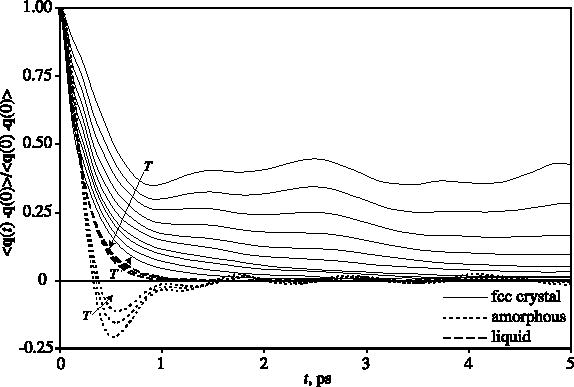
\includegraphics[height=4.5cm]{chapters/chapter5/figures/McGaughey-argon-acf.pdf}}
        \hfill
        \subfigure[\label{fig:argon-gk-phases-kappa}]{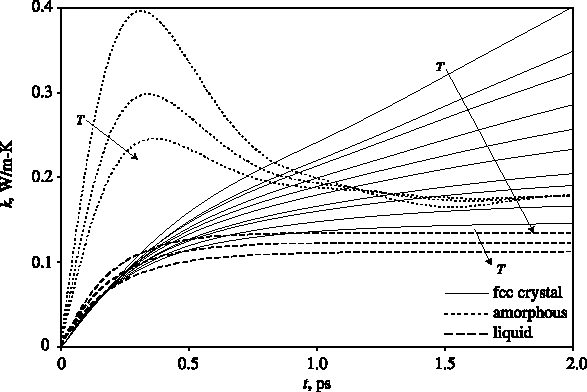
\includegraphics[height=4.5cm]{chapters/chapter5/figures/McGaughey-argon-kappa.pdf}}
    \end{center}
	\caption{(a) Heat current autocorrelation function, Eq.~\eqref{eq:JtJ0}, and
    (b) thermal conductivity as a function of the upper integration limit, Eqs.~(\ref{eq:Lij-integralT}-\ref{eq:kappa-integralT}), for three phases of LJ argon. Reproduced from Ref.~\cite{McGaughey2004a}.} \label{fig:argon-gk-phases-examples}
\end{figure}

\citet{McGaughey2006,McGaughey2004a} studied the thermal conductivity of LJ argon in different phases: fcc crystal, liquid, and amorphous. In Fig.~\ref{fig:argon-gk-phases-examples} we report the comparisons of the HCACFs of these three phases and their direct GK integrals, Eq.~\eqref{eq:kappa-integralT}. At finite time the HCACFs of solid Ar show the two-stage decay \cite{Ladd1986}, and their extension decreases as the temperature increases, as one would expect due to the decrease of phonons relaxation times. 
Their integral converges to the corresponding value of thermal conductivity, however the practical determination of $\kappa$ may be quite subjective. Actually, in the majority of the GK studies reported in the literature, the criteria used to choose an upper limit of integration is not specified, so we guess that they are often based on simple assumption of convergence ``by sight''. 
A few exceptions are listed in the following. For example, the ``first dip'' (FD) method, proposed by \citet{Li1998}, specifies the upper limit of integration by setting the upper limit of integration to be the first time at which the calculated HCACF goes negative. FD may give acceptable results in solid and liquid argon, but it is not suitable to the amorphous phase and in systems with multi-atom unit cell, where the HCACF oscillates wildly around zero before slowly fading out. 

In the case of unit cells with multiple atoms, where intramolecular vibrations manifest as fast oscillations in the HCACF, again, the EF method is not suited to determine $\kappa$. A rather arbitrary compromise was used by \citet{McGaughey2004b}: the GK integral function, Eq.~\eqref{eq:Lij-integralT}, is filtered with a running average \cite{MovingAverage} and the value at which it looks to converge is chosen. If the convergence is not clear one chooses to stop the integration at the point at which the oscillations of $L^{ij}(\mathtt{T})$ reach a minimum (neck). 

Other methods to to perform error analysis have been devised, based on either heuristic or rigorous arguments \cite{Howell2012,Chen2010,Jones2012,Wang_gk2017,Oliveira2017}. All require an estimate of an optimal value for the upper limit of integration, which determines a bias in the estimate, and which is in general difficult to obtain. Moreover most of them are specifically conceived and tested on simple crystalline solids, such as silicon, and are not suited to study disordered and complex systems. 
For example, \citet{Jones2012} proposed a heuristic on-the-fly algorithm to detect the convergence of the block average of $\kappa$, but that needs an empirical estimate of the maximum correlation time first, and thus it is not optimal. A similar empirical criterion has also been proposed by \citet{Wang_gk2017}. \citet{Oliveira2017}, instead, proposed a method that analyses the components of the noise of the GK integral and fits them with integral functions, in order to obtain an estimate of the uncertainty on $\kappa$ of graphite. 


\subsection{Exponential fit and thermal conductivity decomposition}  \label{sec:exp-fit-decomposition}
Another technique proposed by some authors is the exponential fit (EF) method, in which a single or multi-exponential function is fitted to the HCACF beyond a certain point (determined on a case-by-case basis) \cite{Che2000a,Li1998,Zhang2015}. An example is the function \cite{Che2000a}:
\begin{equation}
    \langle J(t) J(0) \rangle = A_{\mathrm{ac,sh}} \mathrm{e}^{-t/\tau_{\mathrm{ac,sh}}} + A_{\mathrm{ac,lg}} \mathrm{e}^{-t/\tau_{\mathrm{ac,lg}}},
\end{equation}
where the subscripts ``$\mathrm{ac,sh}$'' and ``$\mathrm{lg}$'' refer to acoustic, short-, and long range. From here the thermal conductivity is then estimated as:
\begin{equation}
    \kappa = \frac{\rOmega}{k_B T^2} (A_{\mathrm{ac,sh}}\tau_{\mathrm{ac,sh}} + A_{\mathrm{ac,lg}}\tau_{\mathrm{ac,lg}})  =  \kappa_{\mathrm{ac,sh}} + \kappa_{\mathrm{ac,lg}}. \label{eq:kappa-2exp-fit}
\end{equation}
\citet{McGaughey2004a} interpreted the two-stage behavior of solid argon's HCACF and the resulting decomposition of the thermal conductivity in the context of the mean phonon relaxation time: $\kappa_{\mathrm{ac,sh}}$ corresponds to the phonons with lowest relaxation times,\footnote{\emph{i.e.} phonons with a mean free path equal to one half of its wavelength, the shortest possible. This is also called the CP limit, a thermal conductivity model developed for amorphous materials \cite{Cahill1989,Cahill1992}.} whereas $\kappa_{\mathrm{ac,lg}}$ corresponds to phonons with longer relaxation times, that make the longer decay time of the HCACF.
This model works fairly well \emph{e.g.} for solid argon \cite{McGaughey2004a}, diamond and carbon nanotubes \cite{Che2000a,Che2000b}, as well as in liquid argon, where a single-exponential decay is found, but does not work well to fit the long tails of the HCACF of silicon \cite{Schelling2002}.

The HCACF of amorphous argon, though, shows a different behavior with respect to the solid an liquid phases. It is very similar to the velocity autocorrelation function and can be interpreted considering the different local environments the atoms experience. In a crystal each atom is immersed in the same local environment and the same is true in a liquid, if we average over time. Conversely, in an amorphous solid each atom has a different local environment: close to its equilibrium position, it experiences the free trajectory of a liquid atom at short time scales; but at slightly larger times it feels the interactions of the other atoms, that change its trajectory, and make the correlation negative. 
The first timescale of the HCACF decomposition, $\tau_{\mathrm{ac,sh}}$, is related to the time it takes for the energy to move between nearest-neighbor atoms, and corresponds to the higher frequencies of the acoustic branches. The $\kappa_{\mathrm{ac,sh}}$ is the only one important in the liquid and amorphous phase, it is a function of the coordination of the atoms and scarcely depends on temperature, whereas $\kappa_{\mathrm{ac,lg}}$ strongly depends on temperature.

When fast oscillations of the HCACF are present, such as in multi-atom unit cells, \citet{McGaughey2004b} attempted to fit the filtered HCACF with Eq.~\eqref{eq:kappa-2exp-fit} plus a sum of oscillating terms, that they associated to the ``optical'' modes of the system. 
%A more advanced fit can be performed in this case using the form \cite{McGaughey2004b}:
%\begin{multline}
%    \langle J(t) J(0) \rangle = A_{\mathrm{ac,sh}} \mathrm{e}^{-t/\tau_{\mathrm{ac,sh}}} + A_{\mathrm{ac,lg}} \mathrm{e}^{-t/\tau_{\mathrm{ac,lg}}} \\
%        + \sum_i B_{\mathrm{op},i} \mathrm{e}^{-t/\tau_{\mathrm{op},i}} \cos(\omega_{\mathrm{op},i},t),
%\end{multline}
%\begin{equation}
%    \begin{aligned}
%        \kappa &= \frac{\rOmega}{k_B T^2} \left(A_{\mathrm{ac,sh}}\tau_{\mathrm{ac,sh}} + A_{\mathrm{ac,lg}}\tau_{\mathrm{ac,lg}} + \sum_i \frac{B_{\mathrm{op},i}\tau_{\mathrm{op},i}}{1+\tau_{\mathrm{op},i}^2\omega_{\mathrm{op},i}^2}\right) \\
%        &= \kappa_{\mathrm{ac,sh}} + \kappa_{acf,lg} + \kappa_{\mathrm{op}},
%    \end{aligned}
%\end{equation}
%where the subscript ``$\mathrm{op}$'' refers to optical phonon modes. 
Nevertheless, this fitting procedure is very difficult and it was found to be unsuitable for materials like amorphous silica, that therefore requires either a direct integration or an alternative approach.


\subsection{Spectral methods}  \label{sec:spectral-methods}
\begin{figure}[!tb]
    \begin{center}
        \subfigure[\label{fig:aSi-expfit}]{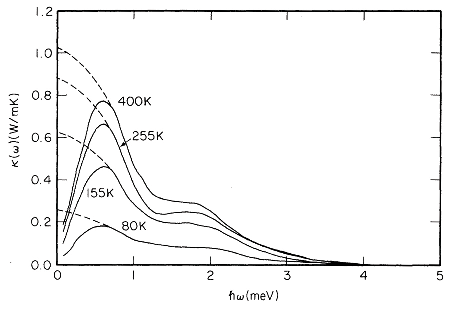
\includegraphics[height=5cm]{chapters/chapter5/figures/Lee-aSi-fit.pdf}}
        \hfill
        \subfigure[\label{fig:cSi-expfit}]{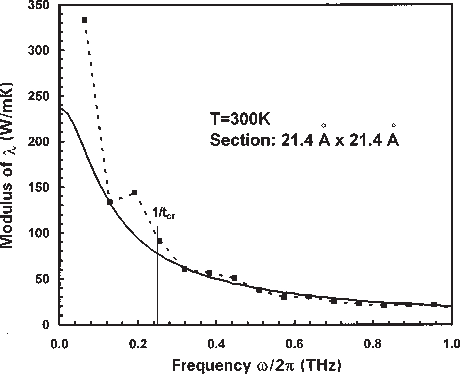
\includegraphics[height=5cm]{chapters/chapter5/figures/Volz-cSi-fit.pdf}}
    \end{center}
	\caption{
	(a) Power spectrum of the heat current of amorphous silicon (solid lines) and Lorentzian fit used to obtain $\kappa$ (dashed lines). Reproduced from Ref.~\cite{Lee1991}. 
	(b) Power spectrum of the heat current of crystalline silicon (dashed line) and fit used to obtain $\kappa$ (solid line). $t_\mathrm{cr}$ is an estimate of the time required for phonons to propagate across the simulation domain ballistically: \citet{Volz2000} argue that for frequencies lower than this mark, phonons will be affected by artificial correlations due to the finite size of the cell and PBC. Reproduced from Ref.~\cite{Volz2000}. 
	} \label{fig:psd-expfit-examples}
\end{figure}
As was shown in Sec.~\ref{sec:Einstein}, the Wiener-Khintchine theorem enables one to express the heat conductivity in terms of the zero-frequency value of the power spectrum of the energy-flux (see Eqs.~(\ref{eq:Wiener-Khintchine}-\ref{eq:GK-S0})):
\begin{equation}
    \kappa = \frac{\rOmega}{2k_B T^2} S (\omega=0). \label{eq:kappa-S0}
\end{equation}
Estimating this limit can be very difficult if the statistical properties of the power spectrum are not taken properly into account, as we will argument in Sec.~\ref{sec:cepstral-analysis}.

Some attempts were made by fitting the low-frequency region of the spectrum with one Lorentzian function (see Fig.~\ref{fig:psd-expfit-examples}) \cite{Lee1991,Volz2000}.
% (or two Lorentzian function, \emph{e.g.} \cite{Hirosaki2002}:
%\begin{equation}
%    S(\omega) = \frac{1}{\mathcal{T}} \left(\frac{A_1\tau_1}{\sqrt{1+\omega^2\tau_1^2}} + \frac{A_2\tau_2}{\sqrt{1+\omega^2\tau_2^2}} \right) ,
%\end{equation}
%or more simply with $A_2=0$ \cite{Lee1991,Volz2000}. 
This is the Fourier transform of an exponential correlation function, hence, not surprisingly, this expression is in good agreement with time integration results when the HCACF is well modeled by one exponential, but does not work when a long tail is present in the HCACF and whenever the exponential fit is inappropriate \cite{Schelling2002}. The same applies if we consider the sum of two Lorentzians, \emph{i.e.} the sum of two exponential functions in the time domain \cite{Hirosaki2002}. 

\citet{Lee1991} and \citet{Volz2000} applied these fits in amorphous and crystalline silicon, respectively, speculating that finite-size effects would affect the low-frequency region. 
The finite size of the simulation cell sets a lower limit to the phonon wavelength that is allowed: only phonons with a wavelength shorter than the cell size are permitted to exist in the simulation domain and can contribute to the thermal conductivity.
Furthermore, the small cell size may introduce artificial autocorrelations that do not exist in real systems, an effect that will be especially strong for phonons with long mean-free paths. 
%\citet{Lee1991} attributed the dip in the heat-current power spectrum of amorphous silicon found at low-frequencies (shown in Fig.~\ref{fig:aSi-expfit}) to this phenomenon, while \citet{Volz2000} attributed it to the apparent divergence of the heat-current power spectrum of crystalline silicon, reported in Fig.~\ref{fig:cSi-expfit}.

\LEnote{**?In our experience, the power spectrum of amorphous silicon does have a shape similar to Fig.~\ref{fig:aSi-expfit}, with a dip at low-frequencies that however does not vanish even when considering much larger sizes. ****FIGURA????******}

We believe that it is not easy to determine \emph{a priori} at what level the power spectrum is affected by finite-size effects. In any case, let us notice that the size-dependence problem in the estimation of $\kappa$ is also present in other methods, such as the direct integration of the GK equation. In general, one should be careful to verify that the chosen simulation cell is big enough for the thermal conductivity to converge. This will also imply that low-frequency region of the power spectrum is correctly reproduced and does not exhibit unphysical features. We will come back on this issue in Ch.~\ref{ch:silica}. 
%In Sec.~\ref{sec:cepstral-analysis} we will start from Eq.~\eqref{eq:kappa-S0} to introduce a more rigorous estimate of the thermal conductivity based on a power spectral analysis with a solid statistical basis.


\subsection{\LE{Estimation from the Einstein relation}}
\LEnote{***************}


\subsection{Final remarks}  \label{sec:data-analysis-remarks}
Many methods have been formulated to estimate the thermal conductivity from the GK equation, but none of them is fully satisfactory. Some of them are optimized to the specific case of crystalline solids or simple liquids, and may be a good choice, however they do not really help much when dealing with amorphous solids. 
Different classes of systems require different approaches to error analysis: in some cases these methods fail to provide rigorous criteria to estimate the accuracy resulting from a given MD trajectory, but in general all of them always require very long simulation times, thus making \abinitio simulations unaffordable. 
In next section we are going to present a novel data-analysis method that will be able to tackle both these problems and to provide us with an efficient and accurate estimator of $\kappa$. This will finally enable us to undertake the study of thermal conductivity of glasses with equilibrium AIMD simulations. 

In Sec.~\ref{sec:exp-fit-decomposition} we saw that one may try to interpret the decay of HCACF in terms of different relaxation times to get insights into the different contributions to the thermal conductivity, though this is not obvious and clear in general. 
The GK equation is a very general result describing the collective dissipative response of any system to a fluctuation, and it has no intrinsic connection to particular transport mechanisms \cite{Howell2012}. 
The frequencies of the power spectrum of the HCACF have been interpreted to be related to the phonon-phonon interactions \cite{McGaughey2004a}. Conversely, in the BTE approach the thermal conductivity is computed by integrating over the frequencies of individual phonons. The difference between these two frequencies is equivalent to that between the mean free path and the corresponding phonon wavelength. 

However, in the light of the gauge invariance principle presented in Ch.~\ref{ch:gauge-invariance}, at this stage it is not very clear how much the HCACF or the power spectrum of the heat current can be interpreted in physical terms. It is evident that different definitions of the microscopic energy density (or atomic energies) will define different energy currents with very different power spectra, the only invariant quantity being their zero-frequency value, \emph{i.e.} the thermal conductivity. 
Whether and how a particular definition can be linked to physical quantities is not yet completely understood. Therefore, extreme caution should be used when making physical interpretations out of a HCACF. 

In conclusion, although the GK method yields a direct estimate of the thermal conductivity, it provides only very indirect information about the mechanisms of heat transport. We believe that different approaches, such as phonon-level methods, \emph{e.g.} methods based on a normal-modes analysis \cite{Esfarjani2011}, may be able to bring better insights into the individual contributions to thermal conductivity, especially in complex or disordered systems. 


%%%%%%%%%%%%%%%%%%%%%%%%%%%%%%%%%%%%%%%%%%%%%%%%%%%%%%%%%%%%%%%%%%%
\section{Cepstral analysis}  \label{sec:cepstral-analysis}

In practice, MD gives access to a discrete sample of the flux process (a \emph{time series}), $J_n = J(n \epsilon)$, $0 \leq n \leq N-1$, where $\epsilon$ is the sampling period of the flux and $N$ the length of the time series, that we assume to be even. 


\subsection{Periodogram}  \label{sec:cepstral-periodogram}
Let us define the discrete Fourier transform of the flux time series as:
\begin{equation}
  \tilde{J}_{k}=\sum_{n=0}^{N-1} \mathrm{e}^{ 2\pi i\frac{kn}{N}} J_n, \label{eq:Jk}
\end{equation}
for $0 \leq k \leq N-1$.\footnote{Here, the convention for the sign in the exponential of the time-to-frequency Fourier transform is opposite to what adopted in Ref.~\cite{Ercole2017} and in most of the signal analysis literature, in order to comply with the convention for the space-time Fourier transforms usually adopted in the Physics literature and in Eqs.~\eqref{eq:kontinuity} and \eqref{eq:Fourier-continuity}.}
The \emph{sample spectrum} $\hat S_k$, aka \emph{periodogram} in the statistics literature, is defined as
\begin{equation}
\hat{S}_{k}=\frac{\epsilon}{N} \left |\tilde{J}_{k} \right |^2, \label{eq:periodogram-def}
\end{equation}
and, for large $N$, it is an unbiased estimator of the power spectrum of the process, as defined in Eq.~\eqref{eq:Wiener-Khintchine}, evaluated at $\omega_k=2\pi\frac{k}{N\epsilon}$, namely: $\langle \hat S_k \rangle = S(\omega_k)$. The reality of the $\hat J$'s implies that $\tilde J_k=\tilde J^*_{N-k}$ and $\hat S_k=\hat S_{N-k}$, so that periodograms are usually reported for $0\leq k\leq \frac{N}{2}$ and their Fourier transforms evaluated as discrete cosine transforms.

The space autocorrelations of conserved currents are usually short-ranged. Therefore, in the thermodynamic limit the corresponding fluxes can be seen as sums of (almost) independent identically distributed stochastic variables, so that, according to the central-limit theorem, their equilibrium distribution is Gaussian. A slight generalization of this argument leads us to conclude that any conserved-flux process, like the heat flux, is Gaussian as well. The flux time series is in fact a multivariate stochastic variable that, in the thermodynamic limit, results from the sum of (almost) independent variables, thus tending to a multivariate normal deviate. This implies that at equilibrium the real and imaginary parts of the $\tilde J_k$'s defined in Eqs.~\eqref{eq:Jk} are zero-mean normal deviates that, in the large-$N$ limit, are uncorrelated among themselves and have variances proportional to the power spectrum evaluated at $\omega_k$. For $k=0$ or $k=\frac{N}{2}$, $\tilde J_k$ is real and $\sim \mathcal{N}\left (0, \frac{N}{\epsilon}S(\omega_k) \right )$; for $k\notin\left\{ 0,\frac{N}{2}\right\}$, $\mathfrak{Re}\tilde{J}_k$ and $\mathfrak{Im}\tilde{J}_k$ are independent and both  $\sim \mathcal{N}\left (0, \frac{N}{2 \epsilon}S(\omega_k) \right )$, where $\mathcal{N} (\mu,\sigma^2)$ indicates a normal deviate with mean $\mu$ and variance $\sigma^2$. We conclude that in the large-$N$ limit the sample spectrum of the heat-flux time series reads:
\begin{equation}
\hat{S}_{k} = S(\omega_k) \,\xi_{k} \,, \label{eq:periodogram-distribution}
\end{equation}
where the $ {\xi}$'s are independent random variables distributed as a $\chi_1^2$ variate for $k=0$ or $k=\frac{N}{2}$ and as one half a $\chi_2^2$ variate, otherwise. Here and in the following $\chi^2_\nu$ indicates the chi-square distribution with $\nu$ degrees of freedom. For the sake of simplicity, we make as though all the ${\xi}$'s were identically distributed as $\xi_k \sim \frac{1}{2} \chi_2^2$ for all values of $k$, thus making an error of order $\mathcal{O}(1/N)$, which vanishes in the long-time limit that is being assumed throughout this section.


\paragraph{Multiple samples}
In many cases of practical interest, multiple time series are available to estimate the power spectrum of a same process, $\{^{p\!}J_n\}$, $p=1, \cdots \ell$. For instance, in equilibrium MD a same trajectory delivers one independent time series per Cartesian component of the heat flux, all of which are obviously equivalent in isotropic systems. In these cases it is expedient to define a mean sample spectrum by averaging over the $\ell$ different realizations,
\begin{equation}
    \begin{aligned}
      {^{\ell\!}\hat{S}}_{k}& = \frac{\epsilon}{\ell N} \sum_{p=1}^{\ell}  \left |{^p\!}{\tilde J}_{k} \right |^2 \\
      & = S(\omega_k) {^{\ell\!}{\xi}_{k}} \,,
    \end{aligned}  \label{eq:mean-periodogram}
\end{equation}
where the ${^{\ell\!}\xi}$'s are $\chi_{2\ell}^2$ variates, divided by the number of degrees of freedom:
\begin{equation}
    ^{\ell\!}\xi_{k}\sim\frac{1}{2\ell}\chi_{2\ell}^{2}, \label{eq:chi-square-nu}
\end{equation}
for $k \notin \{ 0,\frac{N}{2} \}$. 

Eqs.~\eqref{eq:periodogram-distribution} and \eqref{eq:mean-periodogram} show that ${^{\ell\!}}{\hat S_0}$ is an unbiased estimator of the zero-frequency value of the power spectrum, $\langle {^{\ell\!}}{\hat S_0} \rangle = S(0)$, and through Eq.~\eqref{eq:kappa-S0}, of the transport coefficients we are after.
However, this estimator is not consistent, \emph{i.e.} its variance does not vanish in the large-$N$ limit. This is so because a longer time series increases the number of discrete frequencies at which the power spectrum is sampled, rather than its accuracy at any one of them.

\begin{figure}[!tb]
    \centering
    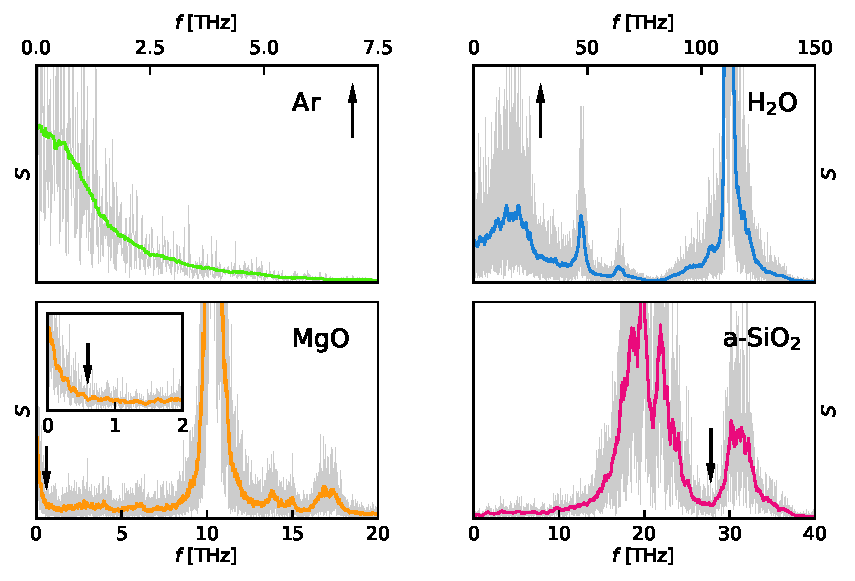
\includegraphics[width=\textwidth]{chapters/chapter5/figures/periodograms.pdf}
    \caption{Sample power spectra of the heat flux computed from MD trajectories for Ar, H$_2$O, a-SiO$_2$ ($100\un{ps}$), and MgO ($500\un{ps}$), obtained directly from Eq.~\eqref{eq:mean-periodogram}, with $\ell=3$ (gray line, see text). The x-axis is frequencies $f=\omega/2\pi$. The solid lines in color correspond to a moving average performed over a narrow frequency window of width $1\un{THz}$, usefult to reveal the main features of the spectrum. The vertical arrows indicate the cutoff frequencies, $f^*$, used for the subsequent cepstral analysis (see Sec.~\ref{sec:cepstral-nyqvist}). The inset in the MgO panel is a magnification of the low-frequency region of the spectrum. Reproduced from Ref.~\cite{Ercole2017}.
    }
    \label{fig:periodograms}
\end{figure}

Fig.~\ref{fig:periodograms} displays the periodograms of the heat fluxes of the four systems presented in Sec.~\ref{sec:data-analysis-4systems} (liquid Ar, liquid H$_2$O, crystalline MgO, and amorphous SiO$_2$), obtained from a $100\un{ps}$ ($500\un{ps}$ for MgO) classical MD trajectory in the NVE ensemble and averaged over the three Cartesian components, showing the extremely noisy behavior of the periodogram as an estimator of the spectrum. 
A consistent estimate of the value of the power spectrum at any frequency can be obtained by segmenting a time series into several blocks of equal length and then averaging over the sample spectra computed for each of them. When the length of the trajectory grows large, so does the number of blocks, thus making the variance of the average arbitrarily small. In practice, the determination of the optimal block size is a unwieldy process that leads to an inefficient determination of the length of the trajectory needed to achieve a given overall accuracy. 
Equivalently, a moving average \cite{MovingAverage} of the periodogram would consistently reduce the statistical noise, as happens in Fig.~\ref{fig:periodograms}, but its \emph{multiplicative} nature in Eq.~\eqref{eq:periodogram-distribution} makes it difficult to disentangle the noise from the signal and may introduce a bias. 
Here we adopt a different approach enabling us to obtain a consistent estimate of the zero-frequency value of the power spectrum from the statistical analysis of a \emph{single} trajectory sample (\emph{i.e.} no block analysis is needed) and such that the estimate of the trajectory length necessary to achieve a given accuracy is optimal.


\subsection{Log-periodogram}  \label{sec:cepstral-log-periodogram}
Spectral density estimation from finite empirical time series is the subject of a vast literature in the statistical sciences, embracing both parametric and non-parametric methods \cite{Stoica2005}. In the following we propose a semi-parametric method to estimate the power spectrum of a stochastic process, based on a Fourier representation of the logarithm of its power spectrum (the ``log-spectrum''). The advantage of dealing with the log-spectrum, instead of with the power spectrum itself, is twofold. First and foremost, the noise affecting the former is \emph{additive}, instead of multiplicative, thus making it simple and expedient to apply linear filters: limiting the number of components of the Fourier representation of the log-spectrum acts as a low-pass filter that systematically reduces the power of the noise and yields a consistent estimator of the log-spectrum at any given frequency. Second, as a bonus, the logarithm is usually smoother than its argument. Therefore, the Fourier representation of the logarithm of the power spectrum is more parsimonious than that of the spectrum itself.

\begin{figure}
    \centering
    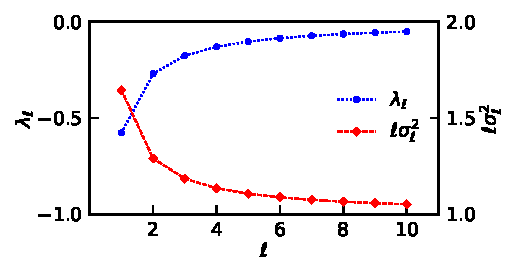
\includegraphics[]{chapters/chapter5/figures/polygamma.pdf}
    \caption{Expectation and variance of the $^{\ell}\lambda$ variables, as defined in Eqs.~(\ref{eq:log-PSD}-\ref{eq:sigma2-ell}), as functions of the number of samples, $\ell$, over which the periodograms are averaged.}
    \label{fig:polygamma}
\end{figure}

Let $^{{\ell\!}}\hat{L}_{k} = \log(^{\ell\!}\hat{S}_{k})$ be the ``\emph{log-periodogram}'' of our time series. By taking the logarithm of Eq.~\eqref{eq:periodogram-distribution}, we can express $^{\ell\!}\hat{L}_{k}$ as:
\begin{align}
    ^{{\ell\!}}\hat{L}_{k} &= \log (^{\ell\!}\hat{S}_{k} ) \nonumber\\
    &= \log\left(S(\omega_k) \right) + \log( ^{\ell\!}{\xi}_k) \nonumber\\
    &= \log\left(S(\omega_k) \right) + {^{\ell\!}\rLambda} + {^{\ell\!}{\lambda}}_{k},  \label{eq:log-PSD}
\end{align}
where
\begin{equation}
    {^{\ell\!}\rLambda} = \left\langle \log( {^{\ell\!}{\xi}}) \right\rangle = \int_0^\infty \log\left (\frac{\xi}{2\ell}\right ) P_{\chi^2_{2\ell}}(\xi) \, d\xi = \psi(\ell)-\log(\ell) \label{eq:lambda-ell}
\end{equation}
is the expected value of the logarithm of the ${^\ell}\hat\xi$ stochastic variables defined in Eq. \eqref{eq:chi-square-nu}, $P_{\chi^2_{2\ell}}$ is the probability density of a $\chi^2_{2\ell}$ variate, $^{\ell\!}{\lambda}_k = \log\left( {^{\ell\!}{\xi}}_k\right) - {^\ell{\rLambda}}$ are zero-mean identically distributed independent stochastic variables, and $\psi(z)$ and is the digamma function \cite{PolyGamma}. 
The variance of the $^{\ell\!}\lambda$ variables is:
\begin{equation}
    \sigma_{\ell}^{2} = \int_0^\infty \log\left (\frac{\xi}{2\ell}\right )^2 P_{\chi^2_{2\ell}}(\xi) \, d\xi - \lambda_{\ell}^2 =\psi'(\ell),\label{eq:sigma2-ell}
\end{equation}
where $\psi'(z)$ is the tri-gamma function \cite{PolyGamma}. 


\subsection{\emph{Ceps}trum and \emph{lif}tering}

\begin{figure}[!tb]
    \centering
    \LE{**** CEPSTRUMS ****}
    %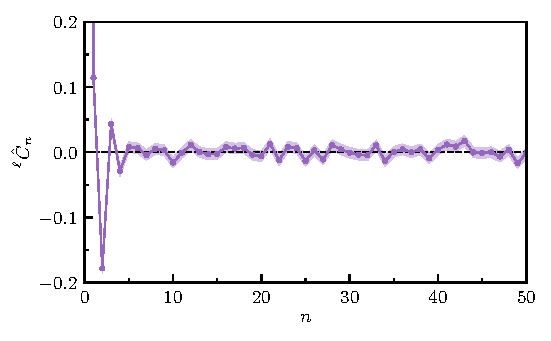
\includegraphics[width=8cm]{chapters/chapter5/figures/handbook_water_cepstrum.pdf}
    \caption{Cepstral coefficients of \LEnote{***...***} computed analyzing the low-frequency region of the periodogram (see Fig.~\ref{fig:periodograms}) and defined in Eq.~\eqref{eq:sample-cepstrum}. }
    \label{fig:cepstrums}
\end{figure}

Eq.~\eqref{eq:log-PSD} explicitly shows that the sample log-spectrum of a time series is equal to the logarithm of the power spectrum one wishes to evaluate (modulo a constant), \emph{plus} a (non-Gaussian) white noise. Whenever the number of (inverse) Fourier components of the logarithm of the power spectrum is much smaller than the length of the time series, applying a low-pass filter to Eq.~\eqref{eq:log-PSD} would result in a reduction of the power of the noise, without affecting the signal. 
In order to exploit this idea, we define the ``\emph{cepstrum}'' of the time series as the inverse Fourier transform of its sample log-spectrum \citep{Childers1977}:
\begin{equation}
  ^{\ell\!} \hat C_{n} = \frac{1}{N}\sum_{k=0}^{N-1} {^{\ell\!} \hat L_{k}} \mathrm{e}^{-2\pi i\frac{kn}{N}}, \label{eq:sample-cepstrum}
\end{equation}
and its coefficients as the \emph{cepstral coefficients} (or ``\emph{que}frencies''). 
A generalized central-limit theorem for Fourier transforms of stationary time series ensures that, in the large-$N$ limit, these coefficients are a set of independent (almost) identically distributed zero-mean normal deviates \citep{Anderson1994,Peligrad2010}. It follows that:
\begin{align}
    ^{\ell\!} \hat  C_{n} &= \lambda_{\ell} \delta_{n0} + C_{n} +  {^{{\ell\!}}{\mu}}_{n},  \label{eq:cepstrogram}\\
    C_{n} &= \frac{1}{N}\sum_{k=0}^{N-1} \log\bigl (S(\omega_k) \bigr ) \mathrm{e}^{-2\pi i\frac{kn}{N}}, \label{eq:C-nohat}
\end{align}
where $^{{\ell\!}}{\mu}_{n}$ are independent zero-mean \emph{normal} deviates with variances $\left\langle {^{{\ell\!}}{\mu}_{n}^2}  \right\rangle$ $=\frac{1}{N}\sigma_\ell^2$ for $n\notin\left\{ 0,\frac{N}{2}\right\}$ and $\left\langle ^{{\ell\!}}{\mu}_{n}^{2}\right\rangle =\frac{2}{N}\sigma_{\ell}^{2}$
otherwise.
This result can be easily checked explicitly by using the definition of the discrete Fourier transform; the non-trivial extra information provided by the central-limit theorem is the asymptotic independence and normality of the $^{\ell}\mu$'s. Similarly to the sample power spectrum, the cepstral coefficients are real, periodic, and even: $\hat C_{n} = \hat C_{N-n}$. 

In some sense, the cepstrum can be interpreted as a sort of correlation function in a pseudo-time domain. However, it differs from the original HCACF for the fact its coefficients are statistically independent and normally distributed, whereas the HCACF values at close time-lags are correlated. 
The word ``\emph{ceps}trum'', obtained by reversing the first four letters of ``spectrum'', was coined to distinguish it from the power spectrum of a signal, and its coefficients essentially give information about the rate of change in the different spectrum bands. This concept has found many applications in voice recognition, pitch detection, characterization of seismic and radar echoes, and more. 


\paragraph{A thermal conductivity estimator}
If the log-spectrum, $\log(S(f_k))$, is smooth enough, the number of non-negligible $C_n$ coefficients in Eq. \eqref{eq:C-nohat} is much smaller than $N$. 
For example, Fig.~\ref{fig:cepstrums} displays the cepstral coefficients of the low-frequency region of the spectrum of the four systems (marked in Fig.~\ref{fig:periodograms}), showing that only the first few coefficients are substantially different from zero. 
Therefore, let us indicate by $P^*$ the smallest integer such that $C_n \approx 0$ for $P^* \le n \le N-P^*$. By limiting the Fourier transform of the sample cepstrum, Eq.~\eqref{eq:sample-cepstrum}, to $P^*$ coefficients, we obtain an efficient estimator of the zero-frequency component of the log-spectrum as:
\begin{equation}
  \begin{aligned}
    ^{\ell\!}\hat{L}_{0}^{*} & = {^{\ell\!}\hat{C}}_{0} + 2 \sum_{n=1}^{P^{*}-1} {^{\ell\!}\hat{C}}_{n} \\
    & = {^{\ell\!}\rLambda} + \log(S_0) + {^{\ell\!} \mu_{0}} + 2 \sum_{n=1}^{P^*-1} {^{\ell\!}} \mu_{n} \,.
  \end{aligned} \label{eq:L0*}
\end{equation}
Inspection of Eq.~\eqref{eq:L0*} shows that $^{\ell\!}\hat{L}_{0}^{*}$ is a normal estimator whose expectation and variance are:
\begin{align}
	\langle {^{\ell\!}}\hat{L}_{0}^{*} \rangle &= \log(S_{0}) + {^{\ell\!}}\rLambda \,, \label{eq:L*} \\
	\sigma_\ell^{*}(P^{*},N)^{2} &= \frac{4P^{*}-2}{N} \sigma_{\ell}^{2} \,. \label{eq:sigma*}
\end{align}
Using Eq.~\eqref{eq:kappa-S0}, we see that the logarithm of the conductivity can be estimated from the cepstral coefficients of the flux time series through Eqs.~(\ref{eq:L0*}-\ref{eq:sigma*}), and that the resulting estimator is always normal with a variance that depends on the specifc system \emph{only} through the number of these coefficients, $P^*$. Notice that the absolute error on the logarithm of the conductivity directly and nicely yields the relative error on the conductivity itself.
%In a sense, $P^*$ can be interpreted like an upper limit of integration of a correlation function in a pseudo-time domain. Again, the actual differences are the well-behaved statistical properties of the cepstral coefficients, opposed to the HCACF's ones.

The value of $P^{*}$ is a property of the stochastic process underlying the time series, and is therefore independent of $N$: for any given value of $P^{*}$ the variance $\sigma_{\ell}^{*2}$ tends to zero in the large-$N$ limit, and $^\ell\hat{L}^*_0-\rLambda_{\ell}$ is thus a consistent estimator of $\log(S_{0})$. In general, all the cepstral coefficients are different from zero and assuming that many of them actually vanish introduces a bias. 
The efficacy of this approach obviously depends on our ability to estimate the number of coefficients necessary to keep the bias introduced by the truncation to a value smaller than the statistical error (that increases with $P^*$), while maintaining the magnitude of the latter at a prescribed acceptable level. 

The choice of $P^*$ is the subject of \emph{model selection} theory, another vast chapter in the statistical sciences \cite{Claeskens2008}. Among the several tests that have been devised to perform this task, we choose the optimization of the Akaike's information criterion (AIC) \cite{Claeskens2008,Akaike1974}, as described in Sec.~\ref{sec:AIC} below, but other more advanced \emph{model selection} approaches \citep{Claeskens2008} may be more effective.

\begin{figure}[!tb]
    \centering
    %\includegraphics[width=8cm]{chapters/chapter5/figures/filtered_psds.pdf}
    \caption{
    Filtered low-frequency region of the power spectrum of \LEnote{******} obtained by limiting the number of cepstral coefficients to various values of $P^*$, Eq.~\eqref{eq:filtered-psd}. $P^*=7$ is the cutoff value suggested by the Akaike's information criterion, Eq.~\eqref{eq:AIC-P}. Grey: the unfiltered periodogram obtained from Eq.~\eqref{eq:periodogram-def}.
    }  \label{fig:filtered-psds}
\end{figure}
%\begin{figure}[!tb]
%    \centering
%    \includegraphics[width=8cm]{chapters/chapter5/figures/kappa_convergence.pdf}
%    \caption{
%    \LEnote{** RIMUOVERE?? **}
%    Thermal conductivity of \LEnote{******} estimated from Eqs.~(\ref{eq:L0*}-\ref{eq:sigma*}) as a function of the cutoff, $P^*$. The colored bands indicate one standard deviation as estimated from theory. The vertical dashed line indicates the value suggested by the Akaike's information criterion, Eq.~\eqref{eq:AIC-P}, $P_A^*$.
%    }  \label{fig:kappa-convergence-Pstar}
%\end{figure}

In Fig.~\ref{fig:filtered-psds} we report the low-frequency region of the spectrum of the four analysed systems obtained by limiting the number of cepstral coefficients to $P^*$:
\begin{equation}
    ^\ell\hat{S}_k^* = \exp\left[ 2\sum_{n=1}^{P^*-1} {}^\ell\hat{C}_n \mathrm{e}^{2\pi i \frac{k n}{N}} + {}^\ell\hat{C}_0 - {}^\ell\rLambda\right], \label{eq:filtered-psd}
\end{equation}
thus showing the filtering effect (actually, ``\emph{lif}tering'' effect, playing on the anagram theme) of this choice.
%Finally, Fig.~\ref{fig:kappa-convergence-Pstar} shows the value of thermal conductivities obtained through Eqs.~(\ref{eq:L0*}-\ref{eq:sigma*}).


\paragraph{Single estimate or multiple estimates?}
\begin{figure}
    \centering
    %\includegraphics{}
    \LEnote{***** FIGURA CONVERGENZA STIMA **********}
    \caption{Caption}
    \label{fig:cesptral-mean-estimators}
\end{figure}
When estimating the value of $L_{0}$ from $\ell$ multiple samples of a same process, one has two options:
\begin{description}
    \item[(a)] compute the mean periodogram ${^{\ell\!}}\hat{S}_k$, Eq.~\eqref{eq:mean-periodogram}, and then compute ${^{\ell\!}}\hat{L}_0^*$ from Eq.~\eqref{eq:L0*}. This leads to Eq.~\eqref{eq:sigma*}:
    \begin{equation}
        \textstyle
        \mathrm{var}\left( {^{\ell\!}}L_0^* \right) = \sigma^*_\ell \left(P^*,N\right)^2 ;
    \end{equation}
    \item[(b)] compute the periodogram of each sample ${^{1\!}}\hat{S}_k$ individually, then weight average the estimator of ${^{1\!}}L_0^*$. This gives
    \begin{equation}
        \textstyle
        \mathrm{var}\left( \frac{1}{\ell} \sum_{i=1}^\ell {^{1\!}}\hat{L}_0^{*i} \right) = \frac{1}{\ell} \sigma_1^* \left(P^*,\frac{N}{\ell}\right)^2 .
    \end{equation}
\end{description}
\LE{In Fig.~\ref{fig:cesptral-mean-estimators} we plot }
the ratio of the corresponding variances, that is $\frac{\sigma_{1}^{2}}{\ell\sigma_{\ell}^{2}} = \frac{\pi^2}{6\ell\psi'(\ell)} > 1$: we conclude that it is more convenient to perform the average over the periodograms (a) instead of on the final estimator (b).

The dependence of $\sigma_{\ell}$ on $\ell$ (displayed in Fig.~\ref{fig:polygamma}) gives us a leverage to reduce the variance of the estimate of $L_{0}$, essentially for free. Suppose one partitions each of the $\ell$ time series of $N$ elements into $m$ segments of $N/m$ elements. When the segments are long enough, the sample average evaluated for each of them has the same variance as the value obtained from the entire trajectory, \emph{i.e.} $\sigma_\ell^{*}(P^{*},N/m)^{2}/m = \sigma_\ell^{*}(P^{*},N)^{2}$, thus providing no improvement. If instead one evaluates ${L}_{0}$ from the mean periodogram averaged over the $\ell \times m$ segments, the corresponding variance would be $\sigma_{\ell m}^2(P^*,N/m)$, which is a decreasing function of $m$ (see Fig.~\ref{fig:polygamma}) and tends to $\frac{4P^{*}-2}{\ell N}$ for $\ell m\gg 1$. In practice the asymptotic behavior $\sigma_{\ell}^{2} = \psi'(\ell) \approx 1/\ell$ is reached for $\ell \gtrsim 6$ ($6\sigma_{6}^{2}\approx 1.09$), and we propose to use $m=6$ segments when only one time series is available ($\ell=1$), thus reducing the standard deviation by a factor $\sqrt{\frac{\sigma_{1}^{2}}{6\sigma_{6}^{2}}}\approx 1.23$. When three times series are available, such as in the simulation of thermal transport in isotropic materials ($\ell=3$), the advantage of segmenting the trajectory by choosing \emph{e.g.} $m=2$ segments would be marginal ($\sqrt{\frac{3\sigma_{3}^{2}}{6\sigma_{6}^{2}}} \approx 1.04$), and we choose therefore to keep $m=1$. 


\subsection{Akaike Information Criterion}  \label{sec:AIC}
We summarize here the AIC, a simple model selection criterion to choose an optimal value of $P^*$, in an automatable way and without any subjective criterion. 

Given a model depending on $P$ parameters, $\theta = \{\theta_{1}, \theta_{2}, \cdots \theta_{P}\}$, the AIC \cite{Claeskens2008,Akaike1974} is a sample statistic defined as
\begin{equation}
    \mathrm{AIC}(P) =-2\max_{\theta}\log\mathcal{L}(\theta,P)+2P,\label{eq:AIC}
\end{equation}
where $\mathcal{L}(\theta,P)$ is the likelihood of the parameters. The optimal number of parameters is determined as the argument of the AIC minimum:
\begin{equation}
    P_A^* \equiv \arg\min_P\mathrm{AIC}(P) . \label{eq:P*}
\end{equation}

In the present case the parameters of the model are the $P$ coefficients $C=\{C_{0},C_{1},\cdots C_{P-1}\}$ as defined in Eq.~\eqref{eq:C-nohat}, and the log-likelihood reads, up to additive terms independent of $P$ and $C$:
\begin{equation}
    2\log\mathcal{L}(C,P) = -\frac{N}{2\sigma_\ell^{2}}\left(C_{0}+\rLambda_{\ell}-\hat{C}_{0}\right)^{2} -\frac{N}{\sigma_\ell^{2}}\sum_{n=1}^{P-1}\left(C_{n}-\hat{C}_{n}\right)^{2} -\frac{N}{\sigma_\ell^{2}}\sum_{n=P}^{N/2} \hat{C}_{n}^{2} .
\end{equation}
Evidently, the above expression is maximized, for given $P$, by $C_{n} = \hat{C}_{n} - \delta_{n0}\rLambda_{\ell}$ for $n=0,1,\cdots P-1$, and the corresponding value of the maximum is: $2\max_C\log\mathcal{L}(C,P) = -\frac{N}{\sigma_\ell^{2}} \sum_{n=P}^{N/2} \hat{C}_{n}^{2}$.
We conclude that the value of the AIC is:
\begin{equation}
    \mathrm{AIC}(P) = \frac{N}{\sigma_\ell^{2}} \sum_{n=P}^{N/2} \hat{C}_{n}^{2} + 2P . \label{eq:AIC-P}
\end{equation}
The value of $P$ that minimizes this expression is the optimal number of parameters in the Akaike sense, $P_A^*$, as defined in Eq.~\eqref{eq:P*}.
\LE{In Fig.~\ref{fig:kappa-convergence-Pstar} the value $P_A^*$ chosen by the AIC for the four systems is indicated.}


\subsection{Nyqvist frequency}  \label{sec:cepstral-nyqvist}
The maximum frequency available for spectral/cepstral analysis is the Nyqvist frequency \cite{Oppenheim1999}, determined by the sampling period $\epsilon$ as $f_{\mathrm{Ny}}=\frac{1}{2\epsilon}$ (\emph{i.e.} angular frequency $\omega_{\mathrm{Ny}}=2\pi f_{\mathrm{Ny}}$). Transport coefficients only depend on the low-frequency behavior of the spectrum, which is independent of $\epsilon$, as long as the latter is small enough as to avoid aliasing effects. For this reason it may prove convenient to eliminate the high-frequency portion of the spectrum ($f>f^*$) by applying a low-pass filter to the time series (\emph{e.g.} a moving average \cite{MovingAverage}) and then resample the latter with a sampling period $\epsilon^*=\frac{1}{2f^*}$, thus resulting in a time series of $N^*=N\frac{f^*}{f_{\mathrm{Ny}}}$ time steps.

The optimal number of cepstral coefficients resulting from Eqs.~\eqref{eq:P*} and \eqref{eq:AIC-P}, as well as the error in the estimate of the transport coefficients resulting from Eq.~\eqref{eq:sigma*}, depends in general on the choice of the cutoff frequency, $f^*$. The smaller $f^*$, the smaller will presumably be the number of cepstral coefficients necessary to describe the log-spectrum to any given accuracy over such a shorter frequency range. However, the shorter length of the filtered time series, $N^*$, results in an increased variance of the estimator $^\ell{\hat L^*_0}$ defined in Eq.~\eqref{eq:L0*}, according to Eq.~\eqref{eq:sigma*}. Numerical experiments performed on the MD data reported in Sec.~\ref{sec:cepstral-benchmarks} and Fig.~\ref{fig:kappa_vs_fstar} show that both the estimated value of $^\ell{\hat L^*_0}$ and its variance are actually fairly insensitive to the value chosen for the cutoff frequency, $f^*$, provided that the power spectrum of the re-sampled time series faithfully features the first band of the original spectrum (\emph{i.e.} the first prominent feature) and that this band is not too peaked at the origin.


\subsection{Data analysis work-flow (solids and one-component fluids)}  \label{sec:cepstral-workflow-1comp}
We summarize the steps leading to the estimation of thermal conductivity by the \textit{cepstral analysis} method, in order to highlight the simplicity of its practical implementation.
\begin{enumerate}
    \item From a MD simulation compute the energy flux time series $J_n^i$, $i=1,\cdots\ell$ (usually $\ell=3$ cartesian components).
    \item Compute the discrete Fourier transform of the fluxes, $\tilde{J}_k^i$, and the mean-periodogram $^{\ell\!}\hat{S}_k$ from Eqs.~\eqref{eq:periodogram-def} and \eqref{eq:mean-periodogram}, and smooth it out using \emph{e.g.} a moving average \cite{MovingAverage} performed over a narrow frequency window, so as to reduce the statistical noise to a level where the shape of the power spectrum of the underlying process can be appreciated.\footnote{Mind the difference between the moving average performed in the frequency domain to smooth out the power spectrum and that performed in the time domain, as suggested before, and acting as a low-pass filter. Spectral smoothing using a moving average in the frequency domain is common practice in the analysis of time series, and it actually provides a consistent estimator of the power spectrum. In fact, the number of frequencies falling within a window of given width increases linearly with the length of the series, so that the variance of the average decreases as the inverse of the product of the length of the series times the width of the window. The resulting spectral estimate is however biased by the variation of the signal within the window, thus strongly reducing the width of the windows that can be afforded. Moreover, both the bias and the statistical error are difficult to estimate, due to the multiplicative nature of the noise; therefore neither the plain periodogram nor a running average thereof are adequate for a quantitative estimate of the zero-frequency value of the power spectrum, which is proportional to the transport coefficient we are after.}
    \item Only a selected low-frequency region shall be used in the next steps (see Sec.~\ref{sec:cepstral-nyqvist} and \ref{sec:cepstral-benchmarks} for a detailed discussion): choose a cutoff frequency, $f^*$, so as to encompass the first band of the smoothed power spectrum. 
    \item Compute the log-periodogram ${^{\ell\!}}\hat{L}_k = \log({^{\ell\!}}\hat{S}_k)$.
    \item Compute the inverse discrete Fourier transform of the result to obtain the cepstral coefficients ${^{\ell\!}}\hat{C}_n$, Eq.~\eqref{eq:sample-cepstrum}. 
    \item Apply the Akaike Information Criterion, Eqs.~\eqref{eq:P*} and \eqref{eq:AIC-P}, to estimate the number of cepstral coefficients to retain, $P^*$.
    \item Finally apply Eq.~\eqref{eq:L0*} to obtain ${^{\ell\!}}\hat{L}_0^*$, and evaluate the thermal conductivity as
    \begin{equation}
        \kappa = \frac{\rOmega}{2k_B T^2} \exp\left[\hat{L}_0^* - \psi(\ell) + \log(\ell) \right],
    \end{equation}
    and its statistical error as
    \begin{equation}
        \frac{\rDelta\kappa}{\kappa} = \sqrt{\psi'(\ell) \frac{4P^{*}-2}{N}}.
    \end{equation}
\end{enumerate}


\subsection{Benchmarks}  \label{sec:cepstral-benchmarks}
The cepstral analysis method just presented has been implemented in a Python package, \textsc{ThermoCepstrum} \cite{thermocepstrum}, and benchmarked for the calculation of the thermal conductivity of the four representative systems presented in Sec.~\ref{sec:data-analysis-4systems}: liquid Ar, liquid H$_2$0, crystalline MgO and amorphous SiO$_2$.
After equilibration, data were collected in the NVE ensemble for trajectories whose length was chosen so as to represent realistic simulation runs that could be afforded using \emph{ab initio} MD ($\mathcal{T} = 100\un{ps}$ for Ar, H$_2$O, and a-SiO$_2$, and $\mathcal{T} =500\un{ps}$ for MgO). 
In order to compare our estimates of the transport coefficients and their statistical errors with reliable and statistically significant reference data, in all cases we ran much longer ($\approx 50\un{ns}$) simulations. 
This allowed us to compare our predicted conductivities with accurate values estimated from the direct integration of the GK equation, Eqs.~\eqref{eq:Lij-integralT} and \eqref{eq:kappa-integralT}, as obtained from a block average \cite{Frenkel2001} performed over the long trajectory (see Sec.~\ref{sec:direct-integration}). 
In addition, we could collect abundant statistics of our estimator for the transport coefficients, Eq.~\eqref{eq:L0*}, and validate its normal distribution specified by Eqs.~\eqref{eq:L*} and \eqref{eq:sigma*}. 

The periodograms of one segment of each system are reported in Fig.~\ref{fig:periodograms}, where a moving average in also computed in order to reveal the main features of the power spectrum. 
The values of the cutoff frequencies used for cepstral analysis, $f^*$, are chosen so as to encompass the first prominent feature of the (smoothed) power spectrum. For instance, in H$_2$O and a-SiO$_2$ we choose $f^*\approx 29\un{THz}$ and $f^*\approx 28\un{THz}$, respectively. In MgO we assume $f^*\approx 0.6\un{THz}$, just at the upper edge of the first narrow peak, whereas in Ar there is just one band, corresponding to a purely diffusive behavior of a simple fluid, and we assume $f^*\approx 7\un{THz}$, where the spectrum has exhausted most of the available power, but its value is not yet too small (see Fig.~\ref{fig:periodograms}). The corresponding average numbers of cepstral coefficients given by the optimization of the AIC are: $P_A^*=5$ (Ar), $7$ (H$_2$O), $4$ (MgO), and $31$ (a-SiO$_2$). Later we will display the dependence of the number of optimal cepstral coefficients and of the resulting estimate of the thermal conductivity on the choice of $f^*$, and show that this choice is not critical.

In order to validate our data-analysis protocol, we first computed the heat conductivities from a direct integration of the current autocorrelation function, Eqs.~\eqref{eq:Lij-integralT} and \eqref{eq:kappa-integralT}, combined with standard block analysis over the $50\un{ns}$ long trajectory (see Sec.~\ref{sec:direct-integration}), that will be taken as a reference, obtaining: $\kappa_{\mathrm{ref}} = 0.1965 \pm 0.0015$, $0.970 \pm 0.009$, $19.2 \pm 0.4$, and $2.115 \pm 0.025 \un{W/mK}$, for Ar, H$_2$O, MgO, and a-SiO$_2$, respectively. 
Although our simulations were meant for benchmarking purposes only, and no particular attention was paid to exactly match the simulation conditions of previous work, these data are in fair agreement with the foregoing theoretical results: $\approx 0.19\un{W/mK}$ (Ar) \cite{Argon-FF}, $\approx 0.85\un{W/mK}$ (H$_2$O) \cite{Romer2012}, $\approx 12\un{W/mK}$ (MgO) \cite{MgO-FF}, and $\approx 2.1\un{W/mK}$ (a-SiO$_2$) \cite{Larkin2014}.

\begin{figure}[!tb]
    \centering
    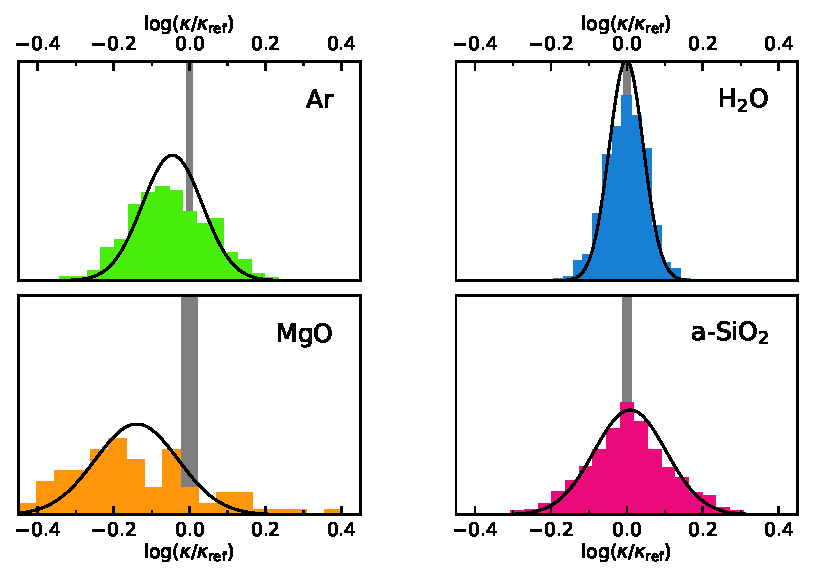
\includegraphics[width=\textwidth]{chapters/chapter5/figures/histograms.pdf}
    \caption{Distributions of the logarithm of the thermal conductivities, $\log(\kappa)$, estimated over multiple MD segments ($100\un{ps}$ for Ar, H$_2$O, and a-SiO$_2$, and $500\un{ps}$ for MgO) extracted from a $50\un{ns}$ long trajectory. The reported data are referred to $\kappa_\mathrm{ref}$, which is the value obtained from a direct integration of the GK equation, combined with standard block analysis over the $50\un{ns}$ trajectory, and represented by the vertical gray bands. The Gaussian curves represent the distributions predicted by the theory, centered at the sample mean. Remember that the absolute error on $\log(\kappa)$ is the relative error on $\kappa$. Reproduced from Ref.~\cite{Ercole2017}.
    }
    \label{fig:histograms}
\end{figure}
\begin{figure}[!tb]
    \centering
    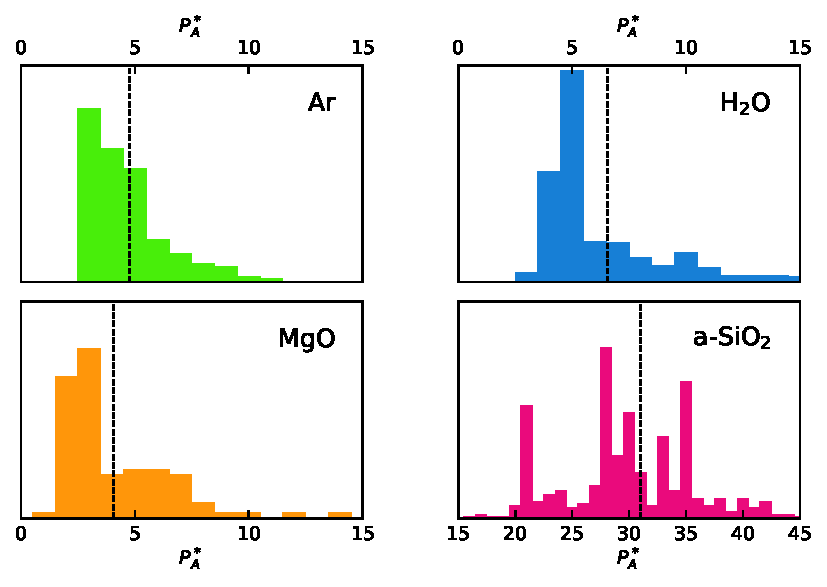
\includegraphics[width=\textwidth]{chapters/chapter5/figures/Pstar_distribution.pdf}
    \caption{Distribution of the optimal numbers of cepstral coefficients, $P_A^*$, as determined by optimizing the Akaike's information criterion, Eqs.~\eqref{eq:P*} and \eqref{eq:AIC-P}, for each segment of the $50\un{ns}$ long MD trajectory, as described in Sec.~\ref{sec:AIC}. The vertical dashed lines indicate the average value of $P_A^*$. Reproduced from Ref.~\cite{Ercole2017}.
    }
    \label{fig:Pstar_distribution}
\end{figure}


\paragraph{Distribution of the estimator of $\kappa$}
In Fig. \ref{fig:histograms} we display the distributions of the values of $\log(\kappa/\kappa_{\mathrm{ref}})$ estimated by applying our protocol to multiple MD segments of $100\un{ps}$ (for Ar, H$_2$O, a-SiO$_2$) and $500\un{ps}$ (for MgO), extracted from the $50\un{ns}$ long trajectory. The optimal numbers of cepstral coefficients, $P^*$, have been redetermined for each segment independently, while the values of the cutoff frequency, $f^*$, which only depends on the qualitative features of the spectrum, have been determined once for all for one of them. The distribution of the resulting number of cepstral coefficients is reported in Fig. \ref{fig:Pstar_distribution}. The observed distributions of $\log(\kappa)$ successfully pass the Shapiro-Wilk normality test \cite{Shapiro1965} (\emph{i.e.} they do not fail it) and the observed sample standard deviations closely match the theoretical values estimated from Eq.~\eqref{eq:sigma*}, as reported in Table~\ref{tab:logkappa-errors}. 
\begin{table}[!htb]
    \centering
    \begin{tabular}{rcc}
                  & \textbf{sample} & \textbf{theory} \\
        \hline
        \textbf{Ar} $(100\un{ps})$       & $0.104$ & $0.079$ \\
        \textbf{H$_2$O} $(100\un{ps})$   & $0.053$ & $0.045$ \\
        \textbf{MgO} $(500\un{ps})$      & $0.17$  & $0.11$ \\
        \textbf{a-SiO$_2$} $(100\un{ps})$ & $0.114$ & $0.095$ \\
    \end{tabular}
    \caption{Observed and theoretical standard deviations of the distributions of $\log(\kappa)$, displayed in Fig.~\ref{fig:histograms}. The theoretical values are obtained from Eq.~\eqref{eq:sigma*}. Remember that the absolute error on $\log(\kappa)$ is the relative error on $\kappa$.}
    \label{tab:logkappa-errors}
\end{table}
Remember that the error on $\log(\kappa)$ is the relative error on $\kappa$: the corresponding absolute errors achievable with a short trajectory of $100$ (Ar, H$_2$O, and a-SiO$_2$) or $500$ (MgO) ps, not to be confused with the long trajectory used to establish the reference data above, are therefore: $\sigma_\kappa \approx 0.015$ (Ar), $0.045$ (H$_2$O), $2$ (MgO), and $0.2$ (a-SiO$_2$) $\mathrm{W/mK}$. This indicates that a \emph{single} and short sample trajectory, such as one that is affordable with \emph{ab initio} MD, is sufficient to achieve and accurately estimate a very decent relative error on the computed transport coefficient. In an attempt to evaluate the thermal conductivity from the direct computation of the GK equation, Eqs.~\eqref{eq:Lij-integralT} and \eqref{eq:kappa-integralT}, and standard block analysis using similarly short MD trajectories, our best estimate of the resulting statistical error was 2-3 times larger than using our protocol (meaning $5-10\times$ longer trajectories to achieve a comparable accuracy) in all cases but liquid Ar, where only a marginal improvement is achieved using our methodology. Much more than this, the standard analysis of MD data depends on a number of hidden parameters, such as the upper limit of the GK integral, Eq.~\eqref{eq:Lij-integralT}, or the width of the blocks for error analysis, that are hard to determine and keep under control, as discussed in Sec.~\ref{sec:direct-integration}. Our method, instead, only depends on a single parameter, the number of cepstral coefficients, whose optimal value can be easily determined from the Akaike's information criterion, or other more sophisticated model-selection methods \cite{Burnham2004,Claeskens2008}, as appropriate.


\paragraph{Bias}
\begin{figure}[!tb]
    \centering
    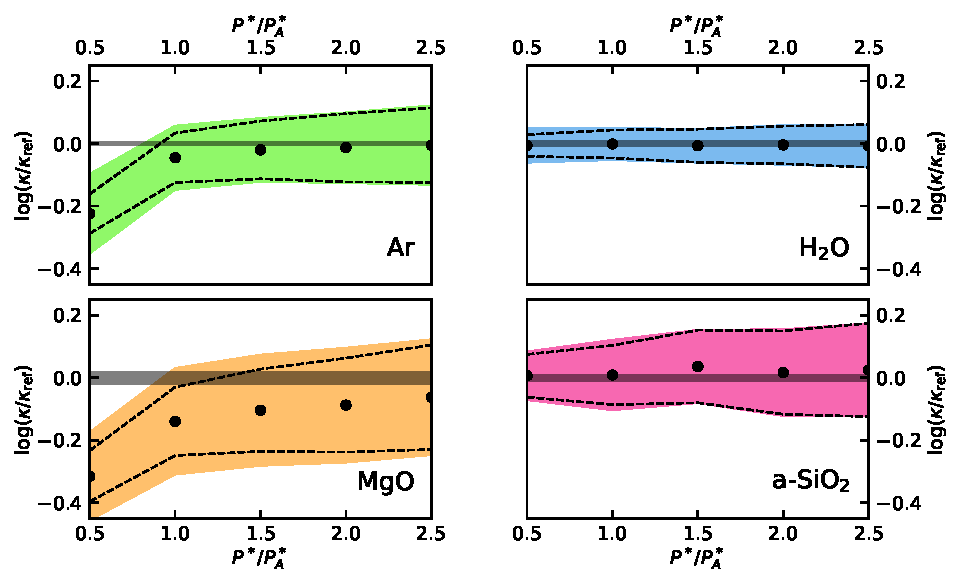
\includegraphics[width=\textwidth]{chapters/chapter5/figures/L-vs-P.pdf}
    \caption{Dependence of $\log(\kappa)$, as estimated from Eq.~\eqref{eq:L0*}, on the number of cepstral coefficients $P^*$. $P_A^*$ is the optimal number of coefficients estimated from the AIC using Eqs.~\eqref{eq:P*} and \eqref{eq:AIC-P}. The black dots represent the mean values of $\log(\kappa)$ computed over multiple MD segments ($100\un{ps}$ for Ar, H$_2$O, and a-SiO$_2$, and $500\un{ps}$ for MgO) extracted from a $50\un{ns}$ long trajectory; the colored bands and dashed lines represent one standard deviation as estimated from the empirical statistics and from Eq.~\eqref{eq:sigma*}, respectively. The reported data are referred to $\kappa_{\mathrm{ref}}$, which is the value of thermal conductivity obtained from a direct integration of the GK equation, combined with standard block analysis over the $50\un{ns}$ trajectory, and represented by the horizontal gray bands. Remember that the absolute error on $\log(\kappa)$ is the relative error on $\kappa$. Reproduced from Ref.~\cite{Ercole2017}.
    }
    \label{fig:L-vs-P}
\end{figure}
\begin{table}[!tb]
    \centering
    \begin{tabular}{ccc}
                  & $\langle\kappa\rangle$ & $\kappa_\mathrm{ref}$ \\
        \hline
        \textbf{Ar}        & $0.1878 \pm 0.0007$ & $0.1965 \pm 0.0015$ \\
        \textbf{H$_2$O}    & $0.969 \pm 0.002$   & $0.970 \pm 0.009$ \\
        \textbf{MgO}       & $16.7 \pm 0.2$      & $19.2 \pm 0.4$ \\
        \textbf{a-SiO$_2$} & $2.131 \pm 0.009$   & $2.115 \pm 0.025$ \\
    \end{tabular}
    \caption{Sample mean of the estimated $\kappa$, computed over the distributions displayed in Fig.~\ref{fig:histograms}; and reference values of thermal conductivity, $\kappa_\mathrm{ref}$, obtained from the direct integration of the GK equation over the $50\un{ns}$ trajectory. Units are $\mathrm{W/mK}$.}
    \label{tab:kappa-bias}
\end{table}
In order to estimate the bias introduced by limiting the number of cepstral coefficients, we examined the sample mean of the estimator of $\kappa$, $\langle\kappa\rangle$, computed over the distributions displayed in Fig.~\ref{fig:histograms}, obtaining the values reported in Table~\ref{tab:kappa-bias}. Comparing these data with the reference data obtained from  the direct evaluation of the GK integral, we see that the bias is negligible for H$_2$O and a-SiO$_2$, very small for Ar, and small but not negligible for MgO. In Fig.~\ref{fig:L-vs-P} we display the dependence of $\log(\kappa/\kappa_{\mathrm{ref}})$ on the number of cepstral coefficients, $P^*$, as estimated from Eq.~\eqref{eq:L0*}. We observe that when the number of cepstral coefficients, $P^*$, is larger than the optimal value determined from the AIC, $P_A^*$, the estimated value of $\kappa$ seems not to depend on $P^*$ for all systems but MgO, for which a slight bias seems to persist, and to a much lesser extent for Ar. Also, Eq.~\eqref{eq:sigma*} seems to slightly underestimate the sample variance for small $P^*$ in these cases. In the case of MgO this behavior is likely due to the difficulty of the AIC to cope with the sharp low-frequency peak in the power spectrum, due to the highly harmonic character and slow decay of the vibrational heat carriers in periodic crystals \cite{Carbogno:2017gc}, thus requiring longer simulation times. In the case of Ar the very small bias observed for $P^* =P^*_A$ may be due to the difficulty of choosing a suitable cutoff frequency when only a single diffusive band is present in the spectrum, and to the divergence of the log-spectrum at high frequency. In all cases, use of the Aikake's information criterion results in a bias that is smaller than the statistical error estimated from an individual short sample trajectory and that can be systematically removed by increasing the value of $P^*$, at the price of increasing the statistical error, if and when needed.


\paragraph{Cutoff frequency $f^*$}
\begin{figure}[!tb]
    \centering
    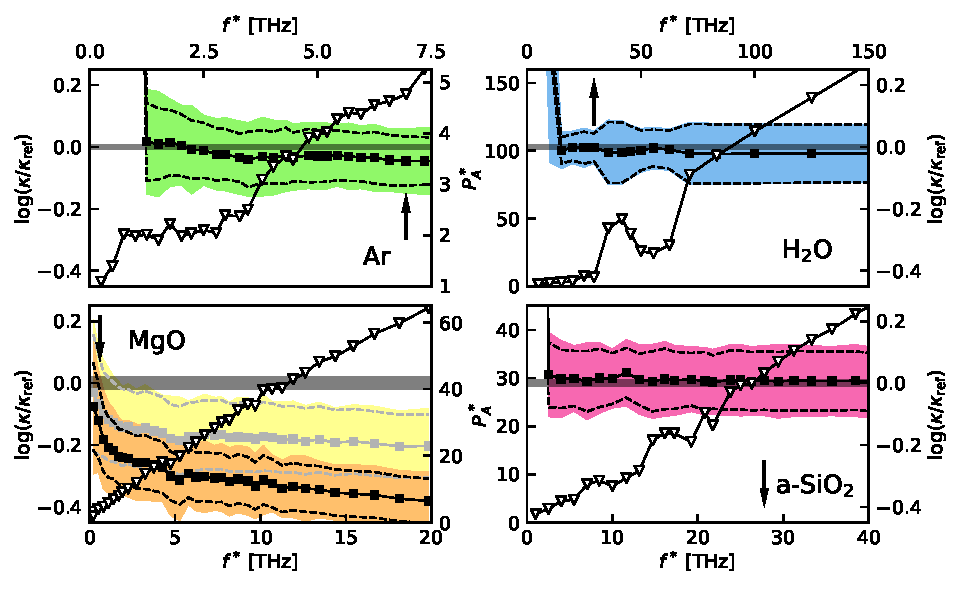
\includegraphics[width=\textwidth]{chapters/chapter5/figures/kappa_vs_fstar.pdf}
    \caption{Triangles: average optimal number of cepstral coefficients, $P_A^*$, as determined by the AIC, Eqs. \eqref{eq:P*} and \eqref{eq:AIC-P}, as a function of the cutoff frequency used for cepstral analysis, $f^*$ (see discussion just after Eq. \eqref{eq:AIC-P}). Squares: $\log(\kappa)$ resulting from a given choice of $f^*$ and of the corresponding value of $P_A^*$. All the values are averages performed over multiple $100\un{ps}$ long segments ($500\un{ps}$ for MgO) extracted from a $50\un{ns}$ long MD trajectory, as discussed in the text. The colored bands indicate the sample standard deviation and the dashed lines that resulting from our theoretical analysis (see Eq. \eqref{eq:sigma*}). The vertical arrows indicate the cutoff frequencies, $f^*$, used for the cepstral analysis in this paper (see Fig. \ref{fig:periodograms} and text). In the case of MgO, the data indicated with lighter colors are obtained using a number of cepstral coefficients twice as large as that provided by the AIC, $P^*=2P_A^*$. The data are referred to $\kappa_{\mathrm{ref}}$, which is the value of thermal conductivity obtained from direct integration of the GK equation over the $50\un{ns}$ trajectory, and represented by the horizontal gray bands. Remember that the absolute error on $\log(\kappa)$ is the relative error on $\kappa$. Reproduced from Ref.~\cite{Ercole2017}.
    }
    \label{fig:kappa_vs_fstar}
\end{figure}
In Fig.~\ref{fig:kappa_vs_fstar} we report the dependence of the optimal number of cepstral coefficients, $P_A^*$, as a function of the cutoff frequency, $f^*$, along with the dependence of the resulting estimate of $\log(\kappa/\kappa_{\mathrm{ref}})$. $P_A^*$ increases (roughly linearly) with $f^*$. Notwithstanding, the estimated value of the heat conductivity, as well as its variance, is fairly insensitive on the precise value of $f^*$ as long as the latter is large enough as to encompass the lowermost prominent feature of the spectrum. 
Some more comments are in order for MgO. In this case the high thermal conductivity, due to the strong harmonic character of slowly decaying phonon modes, manifests in the form of a narrow peak centered at $f=0$, followed by a broad plateau that carries little spectral weight. This feature determines a more pronounced increase in the number of significant cepstral coefficients as $f^*$ increases and a corresponding increase of the bias when keeping $P^*$ at the value given by the AIC. In this case, the AIC is a less reliable indicator of the number of cepstral coefficients necessary to keep the bias low. By increasing this number by a factor of two or more, the bias decreases, as indicated by the results reported in lighter colors in Fig.~\ref{fig:kappa_vs_fstar}, and eventually vanishes, as shown in Fig.~\ref{fig:L-vs-P}.


\paragraph{Trend with simulation length}
The estimate of $\kappa$ of Ar, H$_2$O, and a-SiO$_2$ obtained from a \emph{single} trajectory segment of $100\un{ps}$ is very good. As a function of the cutoff frequency $f^*$, $\log(\kappa)$ oscillates around an average value that is compatible with the distributions of Fig.~\ref{fig:histograms}. 
Using a longer trajectory segment the magnitude of these oscillations decreases, making the estimate of $\kappa$ more stable at different $f^*$, which is compatible with the reduced variance of its distribution. 
In the case of MgO, instead, it appears that by increasing the trajectory length $N$ the bias decreases, and the value of $\log(\kappa)$ becomes less and less dependent upon the $f^*$ choice, if we set $P^*=P_A^*$. 
The number of frequencies used for the cepstral analysis is equal to $N/2$, and the frequency resolution is $\Delta f = \frac{1}{N\epsilon}$. 
In a crystalline system like MgO, the long-living phonon modes manifest themselves as a slowly decaying HCACF (\emph{i.e.} a long autocorrelation time) and a sharp peak at $f\approx 0$ in the spectrum. In order to adequately sample the low-frequency region, a longer trajectory is thus required. 
Whether it is possible to define a minimum simulation length necessary to optimize the estimate of $\kappa$ in such critical cases is an issue that should be studied more extensively, possibly by analyzing synthetic analytic stochastic time series that can reproduce similar power spectra. 
We believe that our model selection criterion can be improved to perform better in this critical class of systems. 

There are two filtering operations that can possibly introduce some spurious effect into the estimate of $\kappa$. 
The first is the low-pass filter applied to the time series before resampling, usually a moving average, that is a rectangular window. 
The type of filter used in this instance will affect the highest frequencies of the spectrum of the resampled heat current (due to aliasing effects and to an effect called \emph{spectral leakage}). 
The second effect happens when we cut off the cepstrum at $P^*$. Setting a hard cutoff at $P^*$ will result in a low-filtered signal equal to the original log-periodogram convolved with a sinc function (the Fourier transform of a rectangular window). This may not be the optimal choice and the estimated log-periodogram will be affected by this, in a certain measure. 
Therefore, both these filtering operations may add some subtle effects to the estimate of $\kappa$ and should be studied more extensively, in the future. 



%%%%%%%%%%%%%%%%%%%%%%%%%%%%%%%%%%%%%%%%%%%
\section{Multi-component fluids}  \label{sec:data-analysis-multicomponent}
In Sec.~\ref{sec:multi-component} we have seen that in a fluid made of $Q$ atomic species there are in general $Q$ macroscopic fluxes interacting with each other through Onsager's phenomenological equations, Eq.~\eqref{eq:onsager}, not counting the different Cartesian components that do not interact amongst themselves because of space isotropy. A MD simulation thus samples $Q$ stochastic processes, one for each interacting flux, that we suppose to be stationary. These processes can be thought of as different components of a same multivariate process. 
Therefore, we can easily generalize the cepstral analysis method presented in Sec.~\ref{sec:cepstral-analysis} to these systems \cite{Bertossa2018}.


\subsection{Cepstral analysis}  \label{sec:cepstral-multicomponent}
As in Sec.~\ref{sec:cepstral-analysis}, for the sake of generality we suppose to have $\ell$ independent samples of such a process, described by a multivariate time series of length $N$: $\{ ^{p\!}{J}^i_n \}$; $p=1,\dots \ell$; $i=1,\dots Q$; $n=0,\dots N-1$. Stationarity implies that $\langle {J}^i_n\rangle $ does not depend on $n$ and that $\langle {J}^i_n {J}^j_m \rangle$ only depends on $n-m$. We will further assume that $\langle {J}^i_n\rangle =0 $ and that $\langle {J}^i_n {J}^j_0 \rangle$ is an even function of $n$, which is the case when ${J}^i$ and ${J}^j$ have the same signature under time-reversal. By combining Eq.~\eqref{eq:multi_kappa} with Eq.~\eqref{eq:GK-S0}, we see that in order to evaluate the thermal conductivity in the multi-component case we need an efficient estimator for $\left ( S^{-1}_0\right )^{11}$, where $S^{kl}_0=S^{kl}(\omega=0)$ is the zero-frequency cross-spectrum of the relevant fluxes, ordered in  such a way that the energy one is the first.

Similarly to the one-component case, we define a mean sample cross-spectrum (or \emph{cross-periodogram}) as
\begin{equation}
 ^{(\ell Q)\!}\hat{S}_k^{ij} = \frac{1}{\ell} \sum_{p=1}^{\ell} \frac{\epsilon}{N} \left({}^{p\!}\tilde{J}_k^i\right)^* {}^{p\!}\tilde{J}_k^j .
\end{equation}
By discretizing Eq.~\eqref{eq:Sij(omega)} we see that $^{(\ell Q)\!}\hat{S}_k^{ij}$ is an unbiased estimator of the cross-spectrum, $\left \langle {}^{(\ell Q)\!}\hat{S}_k^{ij} \right \rangle = S^{ij}\left (\omega_k= \frac{2\pi k }{N\epsilon}\right )$. As it was the case for univariate processes, in the large-$N$ limit the real and imaginary parts of $\tilde J^i_k$ are normal deviates that are uncorrelated for $k\ne k'$. We conclude that the cross-periodogram is a random matrix distributed as a complex Wishart deviate \citep{Goodman1963a,Goodman1963b}:
\begin{equation}
  {}^{(\ell Q)\!}\hat{S}_k \sim \mathcal{CW}_Q \left(S(\omega_k), \ell\right). \label{eq:ComplexWishart}
\end{equation}
The notation $\mathcal{CW}_Q \left(S, \ell \right)$ in Eq.~\eqref{eq:ComplexWishart} indicates the distribution of the $Q\times Q$ Hermitian matrix
${}^{(\ell Q)\!}\hat{S}^{ij} = \frac{1}{\ell}\sum_{p=1}^\ell  {}^{p\!}{X}^i \, {}^{p\!}{X}^{j*}$,
where $\{ {}^{p\!}{X}^i \}$ ($p=1,\cdots\ell$, $i=1, \cdots Q$) are $\ell$ samples of an $Q$-dimensional zero-mean normal variate whose covariance is $S^{ij} = \langle X^i X^{j*} \rangle $.

Similarly to the real case, a Bartlett decomposition \citep{kshirsagar1959} holds for complex Wishart matrices \citep{Nagar2011}, reading:
\begin{equation}
{}^{(\ell Q)\!}\hat{S} = \frac{1}{\ell} \mathcal{S} R R^\top \mathcal{S}^{\dagger},  \label{eq:S_cholesky}
\end{equation}
where ``$\top$'' and ``$\dagger$'' indicate the transpose and the adjoint of a real and complex matrix, respectively; $\mathcal{S}$ is the Cholesky factor of the covariance matrix, $S= \mathcal{S} \mathcal{S}^{\dagger}$, and $R$ is a real lower triangular random matrix of the form
\begin{equation}
 R =
 \begin{pmatrix}
 c_1 & 0 & 0 & \cdots & 0\\
 n_{21} &  c_2 &0 & \cdots& 0 \\
 n_{31} &  n_{32} &  c_3 & \cdots & 0\\
\vdots & \vdots & \vdots &\ddots & \vdots \\
 n_{\smallQ1} & n_{\smallQ2} & n_{\smallQ3} &\cdots & c_\smallQ
 \end{pmatrix},
\end{equation}
where $c^2_i \sim \chi^2_{2(\ell-i+1)}$ and $ n_{ij}\sim \mathcal{N}(0,1)$. We stress that $R$ is independent of the specific covariance matrix, and only depends upon $\ell$ and $Q$. In particular it is independent of the ordering of the fluxes $J^i$. By expressing the $QQ$ matrix element of the inverse of $^{(\ell Q)}\hat{S}$ in Eq.~\eqref{eq:S_cholesky} as the ratio between the corresponding minor and the full determinant, and using some obvious properties of the determinants and of triangular matrices, we find that:
\begin{equation}
\frac{\ell}{\left({}^{(\ell Q)}\hat{S}_k^{-1}\right)^{\smallQ\smallQ}} = \frac{1}{\left(S_k^{-1}\right)^{\smallQ\smallQ}} c^2_\smallQ, \label{eq:S-1_choleskied}
\end{equation}
As the ordering of the fluxes is arbitrary, a similar relation holds for all the diagonal elements of the inverse of the cross-periodogram. We conclude that the generalization of Eq.~\eqref{eq:mean-periodogram} for the multi-component case is:
\begin{equation}
   ^{\ell}\hat{\underline{S}}_{\,k}\equiv\frac{\ell}{2(\ell-Q+1)}\frac{1}{\left( {}^{(\ell Q)}\hat{S}_k^{-1} \right)^{\smallone\smallone}} = \frac{1}{\left(S_k^{-1}\right)^{\smallone\smallone}} \, \xi_k, \label{eq:mean-multi-periodogram}
\end{equation}
where $\xi_k$ are independent random (with respect to $k$) random variables, distributed as
\begin{equation}
  \xi_k \sim
  \begin{cases}
    \frac{1}{\ell-Q+1} \,\chi^2_{\ell-Q+1}  \qquad & \mathrm{for} \; k \in \{0 , \frac{N}{2}\}, \\
 \\
 \frac{1}{2(\ell-Q+1)} \, \chi^2_{2(\ell-Q+1)} \qquad & \mathrm{otherwise}.
\end{cases}
\end{equation}
Starting from here we can apply the cepstral analysis as in the one-component case. The only difference is the number of degrees of freedom of the $\chi^2$ distribution, that becomes $2(\ell -Q+1)$, and a different factor in front of the result. Fig.~\ref{fig:grappa-periodogram} shows an example of multi-component power spectrum for a solution of water and ethanol.

\begin{figure}[!tb]
    \centering
    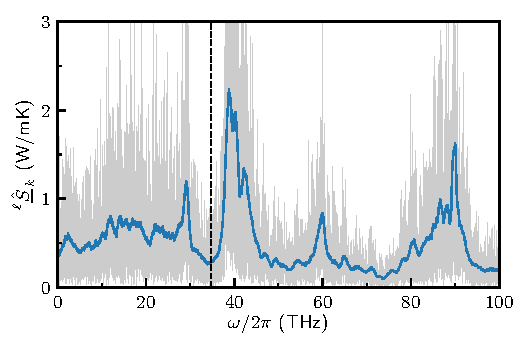
\includegraphics[width=8cm]{chapters/chapter5/figures/psd_water_ethanol_40.pdf}
    \caption{Multi-component power spectrum, as defined in Eq.~\eqref{eq:mean-multi-periodogram}, for a classical flexible model of a solution of water and ethanol $50\un{mol}\%$, obtained from a $100\un{ps}$ trajectory. Grey: $^{\ell}\hat{\underline{S}}_{\,k}$ obtained directly from Eq.~\eqref{eq:mean-multi-periodogram}, with $\ell=3$ and $Q=2$. Blue: $^{\ell}\hat{\underline{S}}_{\,k}$ filtered with a moving average window of width $1\un{THz}$ in order to reveal its main features. The vertical dashed line delimits the low-frequency region used in the subsequent cepstral analysis. Reproduced from Ref.~\cite{Bertossa2018}.
    }
    \label{fig:grappa-periodogram}
\end{figure}

\begin{figure}[!tb]
    \begin{center}
        \subfigure[]{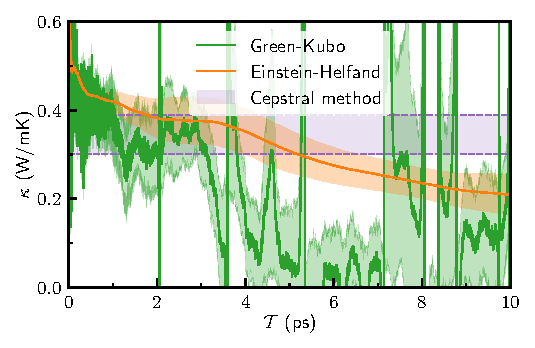
\includegraphics[width=6.8cm]{chapters/chapter5/figures/gk-grappa_capitolo_40.pdf}}
        \hfill
        \subfigure[]{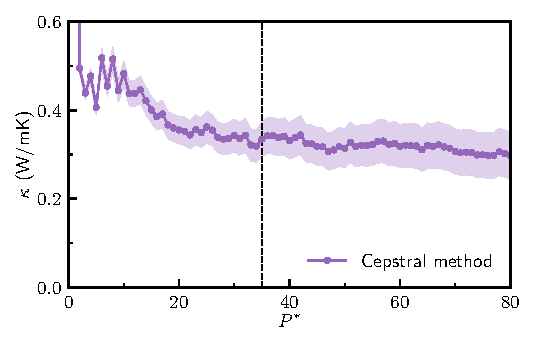
\includegraphics[width=6.8cm]{chapters/chapter5/figures/convergence_water_ethanol_40.pdf}}
    \end{center}
	\caption{Convergence of the multi-component thermal conductivity estimator $\kappa$ using the direct time-integration approach and the cepstral method, for a classical flexible model of a solution of water and ethanol $50\un{mol}\%$, obtained from a $100\un{ps}$ trajectory.
    (a) Direct time-integration approach in its Green-Kubo (green, as obtained from the matrix $L^{ij}(\mathcal{T})\propto\int_0^\mathcal{T} \left\langle J^i(t) J^j(0) \right\rangle dt $) and Einstein-Helfand (orange -- obtained from the  matrix $\left (L^{ij}\right )'(\mathcal{T}) \propto  \int_0^\mathcal{T}\left(1-\frac{t}{\mathcal{T}}\right) \left \langle J^i(t) J^j(0) \right \rangle dt$) formulations. The horizontal purple band indicates the value obtained by the cepstral method.
    (b) Estimate of $\kappa$ with the cepstral method as a function of the number of cepstral coefficients, $P^*$, see Eqs.~(\ref{eq:L0*}-\ref{eq:sigma*}). The dashed vertical line indicates the value of $P^*$ selected by the AIC, Eq.~\eqref{eq:AIC-P}. Reproduced from Ref.~\cite{Bertossa2018}.
    }
    \label{fig:twoCompConvergence}
\end{figure}


\subsection{Discussion}
The method discussed so far shows a fundamental advantage with respect to a na\"ive implementation of direct time-integration approach.
Fig.~\ref{fig:twoCompConvergence} shows the two-component conductivity $\kappa$, obtained via Eq.~\eqref{eq:kappa-integralT} as a function of the upper time-integration limit $\mathcal{T}$, 
\begin{equation}
    \kappa(\mathcal{T}) = \frac{1}{T^2} \left( L^{\smallE\smallE}(\mathcal{T}) - \frac{(L^{\smallE\smallQ}(\mathcal{T}))^2}{L^{\smallQ\smallQ}(\mathcal{T})} \right),  \label{eq:two-comp-kappa-integralT}
\end{equation}
in the case of a water-ethanol solution. Both the Green-Kubo and the Einstein-Helfand definitions of the finite-time expression of Onsager's coefficients (see Eq.~\eqref{eq:Einstein-Helfand-Lij}) are displayed.
Due to thermal fluctuations, the integral of the correlation function becomes a random walk as soon as the latter vanishes, eventually assuming any value. Therefore, there will be a set of times (see Fig.~\ref{fig:twoCompConvergence}) where the term $L^{\smallQ\smallQ}$ at the denominator in Eq.~\eqref{eq:two-comp-kappa-integralT} vanishes, leading to divergences in the evaluation of $\kappa$; an issue not affecting the one-component case. Hence, in such a formulation of the multi-component case, the mean value of the thermal conductivity estimator \textit{in the time domain} does not exist. On the contrary, the multi-component frequency-domain approach presented in this section, and built on sound statistical basis, provides a well defined expression for the estimator of $\kappa$ and its statistical error.


\subsection{Data analysis work-flow (multi-component fluids)}  \label{sec:cepstral-workflow-multicomp}
We summarize the steps leading to the estimation of thermal conductivity by the \textit{cepstral analysis} method for multi-component fluids, in the same way we did in Sec.~\ref{sec:cepstral-workflow-1comp} for solids and one-component fluids. 
\begin{enumerate}
\item From a MD simulation compute the heat flux time series $J_n^1$ and the independent particle fluxes $J_n^q$, $q=2,\dots,Q$.
\item Compute the discrete Fourier transform of the fluxes, $\tilde{J}^{\small i}_k$, and the element $1/(\hat{S}^{-1})^{\smallone\smallone}$. In practice, only a selected low-frequency region shall be used (see \cite{Ercole2017} for a detailed discussion).\footnote{To lighten the notation, we drop the left superscripts of the variables in this subsection.}
\item Calculate $\log\left[1/(\hat{S}^{-1})^{\smallone\smallone}\right]$.
\item Compute the inverse discrete Fourier transform of the result to obtain the cepstral coefficients $\hat{C}_n$.
\item Apply the Akaike Information Criterion, Eq.~\eqref{eq:AIC-P}, to estimate the number of cepstral coefficients to retain, $P^*$.
\item Finally apply Eq.~\eqref{eq:L0*} to obtain $\hat{L}_0^*$, and evaluate the thermal conductivity as
\begin{equation}
\kappa = \frac{\rOmega}{2k_B T^2} \exp\left[\hat{L}_0^* - \psi(\ell - Q+1) + \log(\ell -Q+1) \right],
\end{equation}
and its statistical error as
\begin{equation}
\frac{\rDelta\kappa}{\kappa} = \sqrt{\psi'(\ell -Q+1) \frac{4P^{*}-2}{N}}.
\end{equation}
\end{enumerate}


\section{Outlook}  \label{sec:data-analysis-outlook}
Although a large variety of methods has been formulated in the literature, none of them seems to provide a sufficiently rigorous and accurate estimator of the thermal conductivity that can be applied to different classes of materials and especially to disordered systems. 
The cepstral analysis method introduced in this chapter promises to be a very powerful tool to estimate the thermal conductivity from relatively short MD runs, in a more rigorous way than done so far by other methods. 
Its implementation is straightforward and its use robust, as the only parameter to be determined is the optimal number of cepstral coefficients, using \emph{e.g.} the Akaike's information criterion.
The most impressive results are achieved for disordered systems, \emph{e.g.} liquids and amorphous solids, where a low conductivity results from large cancellations in the integral of a highly oscillatory HCACF, for which all the traditional methods fail or give very subjective results. In these systems, simulation times of the order of $100\un{ps}$ seem sufficient to obtain accuracies of the order of $10\%$ in the estimated thermal conductivities. 

The performance is less spectacular in periodic crystals, where slowly-decaying strongly-harmonic phonon modes require longer simulation times and the ensuing sharp peak in the low-frequency region of the power spectrum requires a larger number of cepstral coefficients than predicted by the optimization of the AIC. Even so, simulation times of the order of a few hundred picoseconds seem sufficient to achieve a comparable accuracy. In the latter case, it is possible that a combination of the methodology introduced here with specialized techniques based on normal-mode analysis, such as that presented in Ref.~\cite{Carbogno:2017gc}, will result in further improvements. 
Leveraging more general (possibly non-Fourier) representations of the log-spectrum of the currents to be analyzed, and replacing the optimization of the AIC with more sophisticated and possibly more efficient approaches, such as \emph{e.g.} weighted multi-model inference techniques \cite{Burnham2004,Claeskens2008}, may also assist in this and other difficult cases. 
Finally, we expect that our methodology will impact on the simulation of any transport phenomena to which the Green-Kubo theory applies, such as ionic conduction, viscosity, and many others: benchmarks on these properties should be performed. 

\LE{This achievement also overcomes the last hurdle towards the quantum simulation of heat transport, which has been considered out of its scope until very recently, due to the long trajectories usually required, and will be particularly important to study strongly anharmonic and/or disordered systems. 
}\LEnote{** controlla se ci sta **}  % Data analysis
\chapter{Thermal conductivity simulations of Silica glass}

\LEnote{*** INTRODUCTION, STATO DELL'ARTE ***}

The simulation of an amorphous system such as a-SiO$_2$ with classical MD and the estimation of its thermal conductivity require a few ingredients. 
First of all, we need a good interatomic force field that faithfully reproduces the structural and dynamical properties of the glass. Both will be important to correctly predict the thermal conductivity, and will be briefly discussed in Sec.~\ref{sec:glass-force-field}.

Second, we need to choose a system size and generate the amorphous structure, a process that is usually performed by melting and equilibrating the system at high temperatures, followed by a cooling phase in which it is gradually brought to the target temperature. At this point the system is equilibrated and data can start to be collected. This ``quenching'' protocol affects the final structural and vibrational properties of the sample, hence we expect the thermal conductivity to be affected by its details. We shall further discuss these points in Sec.~\ref{sec:glass-quenching} and Sec.~\LEnote{**SEZIONE RISULTATI QUENCH**}.

In Sec.~\LEnote{**sezione risultati classici} we will present the method and the results of our classical simulations of vitreous silica. The dependency of the computed thermal conductivity on many of the simulation parameters, such as sample size and quenching protocol, will be discussed. 
Then, one \LEnote{*(a few)*} sample of silica will be chosen and its thermal conductivity studied as a function of the temperature. 

\LEnote{stima errori-->taglia fattibile}

All this classical study will be instrumental in determining the feasibility of \abinitio calculations of thermal conductivity of a-SiO$_2$ using equilibrium MD and the GK equation. One classical sample will be selected and simulated with Car-Parrinello \abinitio MD at four different temperatures. The trajectory thus generated will be used to compute the \abinitio heat current and thermal conductivity using the GK equation. The simulation details and results will be presented in Sec.~\LEnote{SEZIONE QUANTUM}.


%%%%%%%%%%%%%%%%%%%%%%%%%%%%%%%%%%%%%%%%%%%%%%%%%%%%%%%%%%%%%%%%%%%%%%%%%
\section{Classical simulations of a-SiO$_2$}  \label{sec:silica-classical}

\subsection{Force field}  \label{sec:glass-force-field}

The structure of amorphous silica is made of tetrahedra of SiO$_4$, where silicon is at the center, bonded to 4 oxygen atoms located at the vertexes. Each oxygen, in turn, bridges the tetrahedral corners, bonding between two silicon centers. The variation in orientation of adjacent tetrahedra makes the medium and long range structures disordered, forming a typical glass network.

\begin{figure}[!tb]
    \centering
    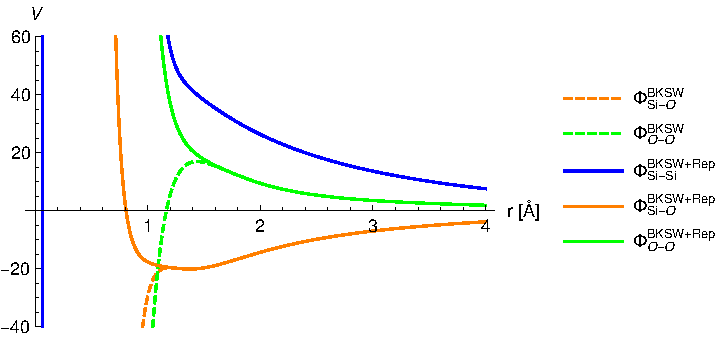
\includegraphics[]{chapters/chapter6/figures/BKSW.pdf}
    \caption{BKS potential with Wolf truncation.}
    \label{fig:BKS-potential}
\end{figure}

One of the most successful force fields for a-SiO$_2$ is the so-called BKS potential \cite{Silica-BKS-1990}. 
The BKS potential was devised by \citeauthor*{Silica-BKS-1990} who fit self-consistent-field Hartree-Fock calculations on small silica clusters, and it has the form...

FORM OF BKS...
\begin{equation}
    BKS, \label{eq:BKS-Wolf}
\end{equation}

TRUNCATION
PARAMETRI USATI (nella sezione risultati)

Let us notices that Si-O bonds are generally considered to have partial ionic and covalent character. The BKS potential is spherical, therefore it does not describe the directional nature of the covalent bond, but it can anyway achieve the tetrahedral structure through a strictly repulsive interaction between oxygen atoms. We can expect that the bond's directionality could be better described by other more sophisticated potentials or by \abinitio methods.

Despite its simplicity, BKS was showed to predict remarkably well many properties of SiO$_2$, among which its complicated phase diagram \cite{Saika2004}. 
Many other force fields have been used in the literature, ranging from simple two-body potentials like the BKS or re-parametrizations of it \cite{Carre2008}, to polarizable force fields \cite{Tangney2002} and reactive force fields (\emph{e.g.} ReaxFF \cite{Yuan2001}). 
Notwithstanding, the BKS potential is still the mostly adopted force field in classical simulations of a-SiO$_2$, thanks to its ability to reproduce faithful glass structures. 
In the following and in Sec.~\ref{sec:glass-quenching} we are going to summarize how the properties of amorphous silica are reproduced by this potential and others.

\paragraph{Structural properties}
\LEnote{For example...}
\citet{Tian2017} compared the structures of silica obtained from different force fields. They quenched a fully melted silica box of density $\rho=2.2\un{g/cm^3}$ from $5000\un{K}$ to $300\un{K}$ at $5\times 10^{12}\un{K/s}$ in the NVT ensemble. 
The BKS and ReaxFF potentials both generate realistic silica structures \cite{Vollmayr1996,Yuan2001}, with radial distribution functions, neutron structure factors, and coordination numbers that reasonably reproduce the experimental observations.
The radial distribution functions present a first sharp peak at $\sim 1.6\un{\angstrom}$ that corresponds to the Si-O bond length, a second peak at $\sim 2.6\un{\angstrom}$ that represents the distance between two O atoms
\LEnote{**grafici g(r) vedi \cite{Bhattarai2016} o altru**}
\LEnote{**rimuovere TETER va...***}
Si-O: $\sim 1.625\un{\angstrom}$, Si-Si: $\sim 1.62\un{\angstrom}$, Si-O: $\sim 2.65\un{\angstrom}$ \cite{Bhattarai2016}.

The coordination numbers can be used to detect coordination defects, by choosing a cutoff length for Si-O pairs of $\sim 2.0\un{\angstrom}$: BKS reproduces a realistic coordination environment for Si and O, with over $99.6\%$ of atoms being normally coordinated (4-fold Si and 2-fold O). ReaxFF, instead, tends to generate more coordination defects, with $\sim 97.5\%$ of normally coordinated atoms.
Nevertheless, the quenching process largely influences the macroscopic and microscopic properties of the generated glass, so we shall comment more on these point later, in Sec.~\ref{sec:glass-quenching}. 

\begin{description}
    \item[Experimental density] $2.202\un{g/cm^3}$
    \item[Experimental thermal expansion coefficient] $\alpha_v \approx 5.5\times 10^{-7}\un{K^{-1}}$. (CHECK)
\end{description}

\paragraph{VDOS}
\begin{figure}
    \centering
    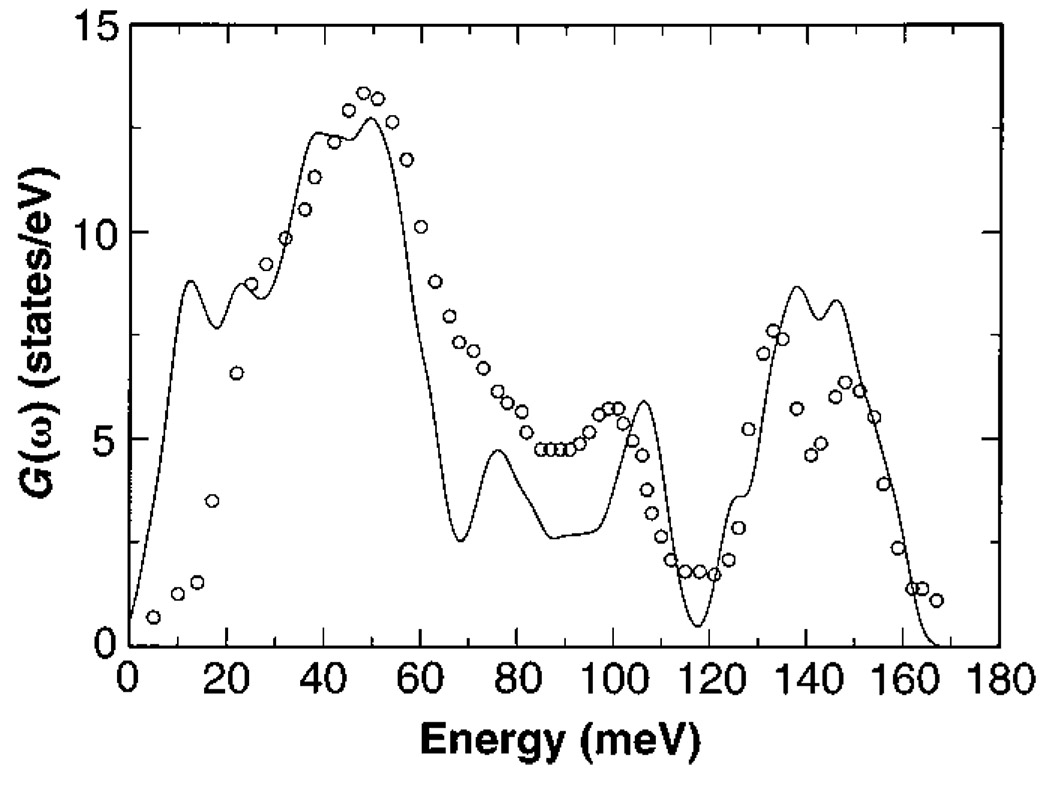
\includegraphics[width=8cm]{chapters/chapter6/figures/Sarnthein_Car_abinitio_VDOS_silica-2.jpg}
    \caption{
    Effective vibrational density of states of an a-SiO$_2$ sample of $72$ atoms at experimental density $2.20\un{g/cm^3}$, computed from AI-CPMD simulations within the local density approximation (solid line), compared to neutron scattering data (circles). Reproduced from Ref.~\cite{Sarnthein1997}.}
    \label{fig:silica-vdos-abinitio}
\end{figure}
\begin{figure}
    \centering
    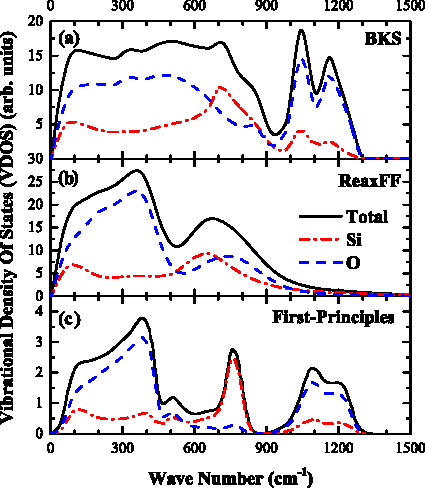
\includegraphics{chapters/chapter6/figures/Tian_VDOS_silica.pdf}
    \caption{
    Total and partial VDOS of a-SiO$_2$ computed for the (a) BKS and (b) ReaxFF, and compared with the (c) first-principle results of \citet{Bhattarai2016}. Adapted from Ref.~\cite{Tian2017}.}
    \label{fig:silica-vdos-classical}
\end{figure}

Besides the structure of the generated sample, what determine the thermal conductivity of the system are its vibrational properties, that are determined by the interaction potential and can be analyzed by the vibrational density of states (VDOS).
Experimentally, the VDOS obtained from neutron scattering shows three significant peaks at about $400\un{cm^-1}$, $800\un{cm^-1}$, and $1100\un{cm^-1}$, that represent the rocking, bending, and stretching modes respectively \cite{Galeener1983}, as shown in Fig.~\ref{fig:silica-vdos-abinitio}.

First principles simulations have shown to successfully reproduce all the principle peaks of the VDOS. \citet{Sarnthein1997} studied a sample of $72$ atoms of a-SiO$_2$ obtained from a quench from the melt with AIMD at experimental density ($2.20\un{g/cm^3}$), within the local density approximation of DFT, and computed the VDOS by diagonalization of the dynamical matrix. Their results, reported in Fig.~\ref{fig:silica-vdos-abinitio}, are in very good agreement with the experiments. The same calculation has been reproduced more recently by \citet{Bhattarai2016} using a $648$-atom model of a-SiO$_2$ (see Fig.\LEnote{Figura articolo Tian, con comparison BKS...}).

Conversely, classical force fields struggle to correctly reproduce the features of the VDOS of a-SiO$_2$. In Fig.~\ref{fig:silica-vdos-classical} we report the VDOS obtained for the BKS and ReaxFF potentials \cite{Tian2017}, compared to an \abinitio calculation \cite{Bhattarai2016}. 
The low-frequency band is dominated by O contributions and agrees well with the results of first-principles simulations and experiments, even though it wrongly elongates up to $600\un{cm^{-1}}$ using the BKS potential. For this model, the modes in the $400-500\un{cm^{-1}}$ range do not agree well with experiment, a sign suggesting that BKS struggles to reproduce correctly the forces over intermediate-range distances \cite{Vollmayr1996,Benoit2002}. 
The intermediate-frequency band of \abinitio simulations is dominated by Si contributions and presents an isolated peak at about $800\un{cm^{-1}}$, but this is not reproduced by the BKS potential, while ReaxFF does not account correctly for the contributions of Si and O atoms. 
The high-frequency band, that corresponds to Si-O stretching vibrations, is well reproduced by the BKS potential, but is notably missing in ReaxFF. 
Therefore we can expect that ReaxFF will provide more realistic predictions of thermal conductivity at room temperature, where thermal conduction is mainly contributed by acoustic-like phonon vibrations whose frequencies are typically below $400\un{cm^{-1}}$ \cite{Bhattarai2016}; whereas the BKS potential will probably be more suitable to study high-temperatures cases, where the contribution of stretching vibrations to thermal conduction increases significantly. 


\subsection{Sample size and preparation}  \label{sec:glass-size}
In contrast to crystals, glasses have a completely disordered non-periodic structure, therefore we should understand what is the minimum sample size that one should simulate to ensure that the distribution of structures is well represented. This is of particular importance in view of performing AIMD simulations, in which the computationally affordable sizes are of the order of a few hundreds of atoms at most. Previous studies have tried to survey this limit. 

A few studies have been performed using \abinitio techniques and they all involved a small sample of $\sim70$ atoms ($\sim 25$ SiO$_2$ units). In the first \abinitio studies, \citet{Sarnthein1995a} performed a quench from the melt completely performed by CPMD, obtaining a first model of vitreous silica. Even though good agreement with experiments was found for some structural, vibrational and electronic properties of this model \cite{Sarnthein1995a,Sarnthein1995b,Sarnthein1997}, a very fast quenching rate (of the order of $10^{15}\un{K/s}$) was used, due to the high computational cost, that may have strongly influenced the results (see Sec.~\ref{sec:glass-quenching} for a deeper discussion). 
Some years later, \citet{Benoit2000} combined classical MD with CPMD: samples generated with the BKS potential (with a quenching rate $\sim 10^{13}\un{K/s}$ were then equilibrated in CPMD. The results from CPMD were similar to the ones of BKS, but in better agreement with experiments with respect to previous studies performed completely in CPMD.
Other five years later, \citet{VanGinhoven2005} studied a set of small silica samples of $72$ atoms generated by the BKS potential and optimized by DFT, and showed that by creating multiple small samples it is possible to achieve a good statistical sampling of structural features consistent with larger simulated glass systems. An ensemble of small samples is necessary to capture the statistical distribution of structures of silica glass, \emph{i.e.} the possible arrangements of its medium range structures. 

Despite these findings, it is not yet clear how much \LEnote{(vibrational properties and )}thermal conductivity may be affected by the size of the sample. Even if we average over a set of small samples, it is possible that $\kappa$ intrinsically requires larger size cells to converge. Finite-size effects similar to the ones found in crystalline solids and briefly described in Sec.~\ref{sec:spectral-methods} may be relevant as well. 
Therefore, a preliminary study on this point should be performed before attempting an \abinitio estimation of the thermal conductivity of a-SiO$_2$. We will present the results of this study in Sec.~\ref{sec:results-class-quench}.


\subsection{Quenching}  \label{sec:glass-quenching}
The properties of the simulated glass may sensibly depend on the quenching process adopted to generate the virtual sample. 
When a supercooled liquid is cooled down so much that the relaxation times of the system exceed the time scale of the (virtual) experiment, the system will be in a nonequilibrium state and undergo a glass transition, provided it does not crystallize. The obtained glass is a nonequilibrium structure whose properties will generally depend on its production history. The \emph{quenching rate} at which it was cooled will determine its macroscopic and, in particular, microscopic properties \cite{Vollmayr1996}. 
For example, the glass transition temperature computed by simulations is significantly higher than the glass transition temperature observed in the laboratory. 
The time scales reachable by computer simulations are many orders of magnitude shorter than the typical time scales of laboratory experiments, hence the minimum quenching rates attainable in classical MD simulations are of the order of $10^{11}-10^{13}\un{K/s}$, a rate that can only be replicated experimentally by strong laser pulses or ion bombardment \cite{Soules2011}.

\paragraph{Macroscopic properties}
\citet{Vollmayr1996} extensively studied the effects of quenching rate on the properties of BKS amorphous silica. They used a sample of $\sim 1000$ atoms at zero pressure, melted it at $7000\un{K}$ and then cooled it down to $0\un{K}$ at different temperature rates $\gamma$, ranging from $10^{12}$ to $10^{15}\un{K/s}$. More recently, \cite{Lane2015} extended their study, reaching cooling rates down to $5\times 10^{9}\un{K/s}$ with microsecond MD simulations of $\sim 13000$ atoms.

\begin{figure}[!tb]
    \centering
    \subfigure[\label{fig:silica-bks-density-anomaly}]{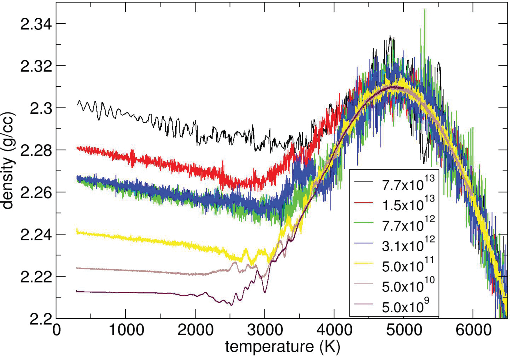
\includegraphics[height=4.6cm]{chapters/chapter6/figures/Lane_density1.pdf}}
    \hfill
    \subfigure[\label{fig:silica-bks-density-temp}]{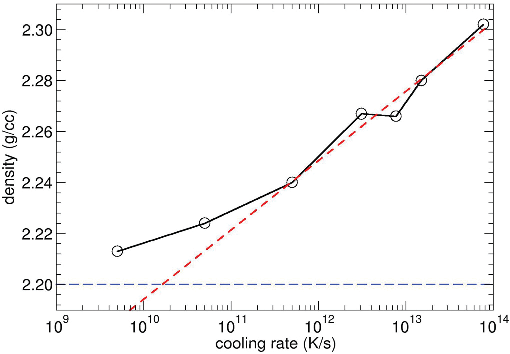
\includegraphics[height=4.6cm]{chapters/chapter6/figures/Lane_density2.pdf}}
    \caption{
    (a) Density vs temperature of a-SiO$_2$, modelled with the BKS potential, for seven quenches completed with linear cooling rates $\gamma$ from $8000\un{K}$ to $300\un{K}$. Silica's density anomaly is visible at high temperatures; density becomes independent of $\gamma$ at $T \gtrsim 4500\un{K}$. 
    (b) Density at $300\un{K}$ as a function of the quench cooling rate $\gamma$. The horizontal dashed line is the experimental value. The red dashed line is a linear extrapolation fit to data above $3\times 10^{12}\un{K/s}$. 
    Reproduced from Ref.~\cite{Lane2015}}
    \label{fig:silica-bks-density}
\end{figure}
The glass transition temperature, that they estimated from the enthalpy curves, increases with $\gamma$. As one can expect, fast cooling rates make the system fall out of equilibrium more quickly during the quench. 
The density $\rho$ of the final sample also depends on the quenching rate: at temperatures below $2000-3000\un{K}$, higher $\gamma$ determine higher densities, as can be observed in Fig.~\ref{fig:silica-bks-density}, and seem to approach the experimental value of $2.202\un{g/cm^3}$. Between $10^{14}\un{K/s}$ and $10^{9}\un{K/s}$ density decreases of about $5\%$. 
This behavior is unusual: in most glasses density increases as cooling rates are slowed. It can be explained by observing the trend at higher temperatures, where the density appears to have a maximum at $T\sim 4800\un{K}$ that does not depend on $\gamma$: this ``density anomaly'' is also observed in experiments, at a much lower temperature of $1820\un{K}$. This discrepancy can be attributed to the BKS potential.
Furthermore, the thermal expansion coefficient at constant pressure, $\alpha_p = \frac{1}{V} \left.\frac{\partial V}{\partial T}\right|_p = -\frac{1}{\rho} \left.\frac{\partial \rho}{\partial T}\right|_p$, increases with $\gamma$.

\paragraph{Microscopic properties}
Microscopic properties are even more affected by the quenching rate. 
By analysing the radial distribution function (RDF) between different species it is possible to observe that a small cooling rate makes the structural order at short and intermediate distances increase, \emph{i.e.} the RDF peaks and minima are sharpened. However, the location of the RDF's peaks is very little affected by $\gamma$ (\emph{i.e.} the Si-O tetrahedra do not change much their size with $\gamma$) and compares quite well with experiment, thus making BKS a good potential to reproduce the short- and medium-range structure of a-SiO$_2$. 
The study of coordination numbers of each atom type shows that local order increases fast with decreasing cooling rate: for example, the number of Si atoms that are 4-fold coordinated with oxygen atoms increases from $95\%$ to $99.5\%$ by decreasing the cooling rate from $10^{15}\un{K/s}$ to $10^{13}\un{K/s}$, and even further at $10^{10}\un{K/s}$.
Since the size of Si-O tetrahedra does not change much their size with $\gamma$, the variation of density with the changes in the cooling rate is due to relative arrangement of neighboring tetrahedra. 
This can be observed in variations of the angle distributions (\emph{e.g.} the O-Si-O angle distribution sharpens by decreasing $\gamma$ and approaches the ideal tetrahedron angle of $109.47^\circ$; the Si-O-Si angle distribution, instead, does not sharpen but shifts to larger angle values, indicating a more open arrangement of tetrahedra, which is consistent with the observed lower density) and rings distributions (rings of size $6$ becomes more frequent with decreasing $\gamma$, indicating that the local structure of the system approaches the one of $\beta$-crystobalite). 
Finally, the two high-frequency peaks of VDOS depend on the quench rate in that their height increases significantly by decreasing $\gamma$, hence improving the agreement with experiment. The low-frequency band, which is quite featureless, does not change very much, and the same applies to the intermediate band, that therefore remains quite in discordance with experimental results. 

\begin{LEtext}
In conclusion, even though these studies have been performed using the BKS potential and not with DFT (for obvious computational reasons), it is very reasonable to assume their results will also hold for AIMD simulations of amorphous silica. 
The demonstrated structure predictions capabilities of the BKS potential and the very large range of time scales analyzed leads us to conclude that a reliable a-SiO$_2$ structure can only be obtained by a ``slow'' quenching process with classical MD. 
However, to our knowledge a study of the dependence of thermal conductivity on the quenching rate has never been attempted and should be performed before starting a first-principles calculation. In Sec.~\ref{sec:results-class-quench} we will present this study. 
\end{LEtext}


\subsection{Thermal conductivity: previous studies}
\paragraph{Non-Equilibrium MD studies}
Many studies of the thermal conductivity of a-SiO$_2$ are based on NEMD simulations, that are strongly size dependent due to scattering of phonons with the heat sink, and thus require the study of its convergence at large cell sizes. 
For example, \citet{Tian2017} simulated a-SiO$_2$ with the BKS potential at $T=300\un{K}$, $\rho=2.2\un{g/cm^3}$, and obtained a value of thermal conductivity of $\kappa=(2.27 \pm 0.06)\un{W/mK}$ at the maximum size simulated, whereas \citet{Coquil2011} obtained $\kappa= (2.10 \pm 0.10)\un{W/mK}$. 

An extrapolation technique is needed to estimate the convergence of $\kappa$ as a function of the length of the simulation cell in the direction of the applied heat flux (or temperature gradient), $L_z$. According to the kinetic theory: $\kappa = \frac{1}{3} c_v v \,l$, where $c_v$ is the lattice specific heat at constant volume, $v$ is the sound velocity, and $l$ is the mean-free path of the phonons. The thermal conductivity can be obtained by linear fitting $1/\kappa$ vs $1/L_z$ and extrapolating the value at $1/L_z=0$ \cite{Schelling2002}. 
Despite being widely applied in the literature, this method has to be adopted with extreme care. Indeed, if the distribution of phonon mean-free paths cannot be approximated by its average value, then the linear dependence of $1/\kappa$ on $1/L_z$ is no longer valid, as higher-order terms are not negligible, as \citet{Sellan2010} ascertained studying Ar and Si crystals. If the considered system sizes are smaller than the largest bulk mean-free paths that dominate the thermal transport, then the linear relationship may not work and the thermal conductivity can be severely underestimated.

In the case of amorphous silica, the maximum phonon mean-free path is quite short ($\sim 6\un{\angstrom}$ \cite{Yu2006}), a fact that may explain why \citet{Tian2017} find the linear fit to work well in this case, allowing them to extrapolate a value of $\kappa=2.5\un{W/mK}$ for the BKS and Teter potentials, and of $1.28\un{W/mK}$ for the ReaxFF potential, at $300\un{K}$. Therefore, the ReaxFF potential seems to best reproduce the experimental value of $\kappa_{exp}\approx 1.3-1.4\un{W/mK}$ at this temperature. 


\paragraph{Equilibrium MD studies}
Few studies have been performed using EMD, probably due to the difficulty in estimating the thermal conductivity from the GK equation, as we already described in Sec.~\ref{sec:data-analysis-methods}.
\citet{McGaughey2004b} was estimated the thermal conductivity of a system of $576$ atoms (\LE{$\rho=***$ at $T\sim \un{K}$}), obtaining a thermal conductivity of $1.96\un{W/mK}$. 
The GK method is much less affected by finite-size effets, and can simulate the bulk with much smaller systems, actually much smaller than the estimated phonon mean-free path \cite{Schelling2002}. As already mentioned in Sec.~\ref{sec:spectral-methods}, the potential finite-size effects of the GK method may be attributed to memory effects, \emph{i.e.} to phonons that, thanks to PBC, reenter the simulation box several times without scattering and hence may introduce artificial correlations. In this case, the heat flux autocorrelation function may not be reliable for times longer than the time required for the passage of the phonon across the simulation cell. 
\LE{**celle usate da McGaughey??**}

\paragraph{Lattice methods????}
\LEnote{******ANYTHING***??}


%%%%%%%%%%%%%%%%%%%%%%%%%%%%%%%%%%%%%%%%%%%%%%%
\section{Classical simulations: Results}
We performed classical MD simulations of amorphous silica using the \textsc{LAMMPS} package \cite{LAMMPS1995}. The BKS potential with Wolf truncation has been implemented as in Eq.~\eqref{eq:BKS-Wolf}. 
Since the potential becomes attractive at very short distances, a repulsive part at short-range has been added to it in order to avoid atoms to get too close to each other: a problem that may arise at high temperatures during melting. This repulsive core has the form:
\begin{equation}
    BKSREPULSIVE, \label{eq:BKS-repulsive-core}
\end{equation}
and has been designed such that the potential and its first and second derivatives are continuous, similarly to Ref.~\cite{Mantisi2012}. The parameters of the potential are reported in Table~\ref{tab:BKS-table}

\begin{table}[!htb]
    \centering
    \begin{tabular}{c|c}
         &  \\
         & 
    \end{tabular}
    \caption{Parameters of the BKS potential defined in Eq.~\eqref{eq:BKS-Wolf} and \eqref{eq:BKS-repulsive-core}.}
    \label{tab:BKS-table}
\end{table}


\subsection{Cepstral analysis}
\paragraph{Dependence on cutoff frequency $f^*$}
(For the chosen sample at experimental density)
(comparison bw normal and vel-renormalized results)

\begin{figure}[!tb]
    \centering
    \subfigure[\label{fig:csilica-sample-expdens-fstar-100ps}]{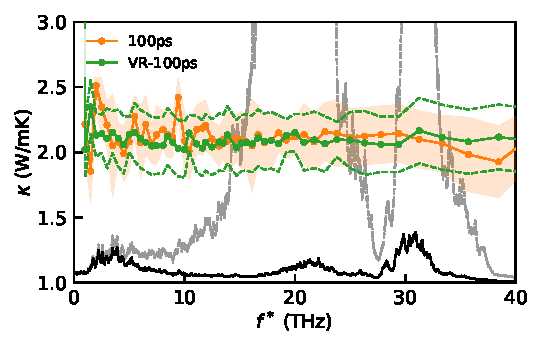
\includegraphics[width=8cm]{chapters/chapter6/figures/silica_expdens_kappa_fstar_VR_100ps.pdf}}
    \subfigure[\label{fig:csilica-sample-expdens-fstar-1ns}]{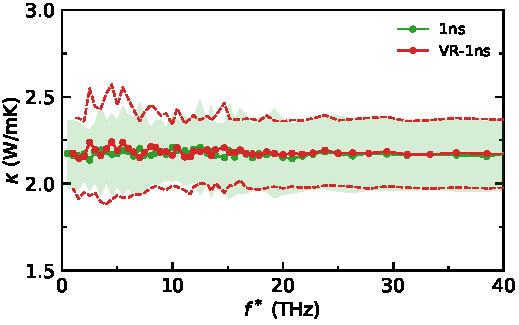
\includegraphics[width=8cm]{chapters/chapter6/figures/silica_expdens_kappa_fstar_VR_1ns.pdf}}
    \subfigure[\label{fig:csilica-sample-expdens-fstar-10ns}]{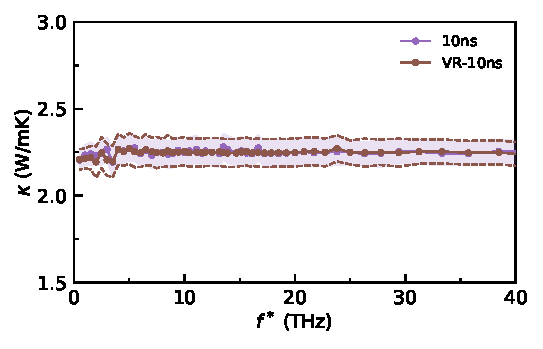
\includegraphics[width=8cm]{chapters/chapter6/figures/silica_expdens_kappa_fstar_VR_10ns.pdf}}
    \caption{Dependence of $\kappa$ on the choice of the cutoff frequency $f^*$, estimated from \emph{one} sample of (a) $100\un{ps}$, (b) $1\un{ns}$, and (c) $10\un{ps}$ of the ``original'' and VR heat flux time series. 
    The original and VR periodograms are reported for reference with grey and black lines, respectively.}
    \label{fig:csilica-sample-expdens-fstar}
\end{figure}
Fig.~\ref{fig:csilica-sample-expdens-fstar} -- stability of $\kappa$ as a function of $f^*$ increases with the length of the trajectory, as its predicted error decreases. The values and errors of $\kappa$ obtained from the VR time series are equivalent to the ones obtained from the original time series, and are slightly more stable with $f^*$. This is probably due to the much smaller power of the power spectrum of the VR heat flux, that may decrease the small artifacts introduced by the low-pass filter applied before resampling. 
Any frequency in the central region of the spectrum can be taken as $f^*$, hence we choose to set $f^*=28\un{THz}$. Conversely, a $f^*$ too small makes $\kappa$ deviate sensibly, due to the fact that the low-pass filter is not strong enough to avoid aliasing effects that modify the spectrum of the resampled time series; instead, a $f^*$ that is too high ($f^*\gtrsim 60\un{THz}$) induces a bias in $\kappa$, due to the fact the log-periodogram diverges to negative values and we start to have problems of numerical precision.


\subsection{Finite-size and quench rate dependence}  \label{sec:results-class-quench}
SIZE EFFECTS:  SMALL SAMPLE PROBLEMS -- SIZE EFFECTS OF GK

\subsection{Volume dependence}
(NEGLECTED)

\subsection{Temperature dependence}
AND THERMAL CURRENT CONTRIBUTIONS (CONV, VIR, X)


%%%%%%%%%%%%%%%%%%%%%%%%%%%%%%%%%%%%%%%%%%%%%%%%%5
\section{Quantum simulations}
QUANTUM

\subsection{Setup}

\subsection{Heat current calculation}
DT HEAT CURRENT

\subsection{Results}
  % Silica
\thischaptertocfalse
\chapter{Conclusions}  \label{ch:conclusions}

\begin{itemize}
    \item GK for complex real systems, interfaces, ...
\end{itemize}  % Conclusions

\appendix

\chapter{Classical definitions of energy flux in solids}  \label{ch:appendix-carbogno}

In this appendix we demonstrate the equivalence between two formulations of the classical energy current in solids, Eqs.~\eqref{eq:J-classical} and \eqref{eq:J-leyla}, by using the gauge invariance principle presented in Sec.~\ref{sec:gauge-invariance}. 

Let us consider the general formula of the energy flux for classical force fields, Eq.~\eqref{eq:J-classical}, and rewrite it in the following way:
\begin{align}
    \mathbf{J}_A^\smallE (\rGamma) &= \frac{1}{\Omega} \sum_n \left( \mathbf{J}_c^\smallE + \mathbf{J}_v^\smallE \right) \nonumber\\
        &= \frac{1}{\Omega} \sum_n \left( \dot{\mathbf{R}}_n \epsilon_n + \mathbf{R}_n \dot{\epsilon}_n \right) , \label{eq:apx-J-classical}
\end{align}
where $\mathbf{J}_c^\smallE$ and $\mathbf{J}_v^\smallE$ are the ``convective'' and ``virial'' components of the energy flux, as defined in Eqs.~(\ref{eq:J-convective}-\ref{eq:J-virial}). 
In solids, the definition of Eq.~\eqref{eq:J-leyla} can be adopted, that can be rewritten as:
\begin{equation}
    \mathbf{J}_B^\smallE(\rGamma) =
       \frac{1}{\rOmega} \sum_{n,m} \mathbf{R}_n^0 \dot{\epsilon}_n , \label{eq:apx-J-leyla}
\end{equation}
where $\mathbf{R}_n = \mathbf{R}_n^0 + \mathbf{u}_n$, $\mathbf{R}_n^0$ denotes the average atomic position of atom $n$, and $\mathbf{u}_n$ its instantaneous displacement. 
According to the gauge invariance theorem (p.~\pageref{th:gauge-invariance}), in order to ensure that $\mathbf{J}_B^\smallE(\rGamma)$ is equivalent to $\mathbf{J}_A^\smallE(\rGamma)$, that is it yields the same thermal conductivity, we just need to prove that their difference is \emph{non-diffusive}, \emph{i.e.} it is a total time derivative of a bounded vector. 
After a few manipulations we have:
\begin{align}
    \mathbf{J}_A^\smallE(\rGamma) - \mathbf{J}_B^\smallE(\rGamma) 
        &= \frac{1}{\Omega} \sum_n \left( \dot{\mathbf{R}}_n \epsilon_n + \mathbf{R}_n \dot{\epsilon}_n - \mathbf{R}_n^0 \dot{\epsilon}_n \right) \nonumber\\
        &= \frac{1}{\Omega} \sum_n \left( \dot{\mathbf{u}}_n \epsilon_n + \mathbf{u}_n \dot{\epsilon}_n \right) \nonumber\\
        &= \frac{1}{\Omega} \frac{d}{dt} \sum_n \dot{\mathbf{u}}_n \epsilon_n ,
\end{align}
where we used the fact that $\dot{\mathbf{R}}_n = \dot{\mathbf{u}}_n$.
The sum $\sum_n \dot{\mathbf{u}}_n \epsilon_n$ is a function of the phase-space that is well-defined in PBC, and it is a bounded quantity, in a solid where atomic diffusion does not occur. Therefore we can conclude that $\mathbf{J}_B^\smallE(\rGamma)$ and $\mathbf{J}_A^\smallE(\rGamma)$ result in the same thermal conductivity. 

The same cannot be concluded for the sole ``virial'' term $\mathbf{J}_v^\smallE$, for which we have that:
\begin{align}
    \mathbf{J}_A^\smallE(\rGamma) - \mathbf{J}_v^\smallE(\rGamma) 
        &= \frac{1}{\Omega} \sum_n \dot{\mathbf{R}}_n \epsilon_n  \nonumber\\
        &= \frac{1}{\Omega} \sum_n \dot{\mathbf{u}}_n \epsilon_n  \nonumber\\
        &= \mathbf{J}_A^\smallE(\rGamma) - \mathbf{J}_B^\smallE(\rGamma) - \frac{1}{\Omega} \sum_n \mathbf{u}_n \dot{\epsilon}_n .
\end{align}
The last two lines are not manifestly expressible as a total time derivative of a bounded vector, therefore the ``convective'' term $\mathbf{J}_c^\smallE$ cannot be neglected \emph{a priori} in a solid. The magnitude of its contribution (and that of the cross-correlations $\langle\mathbf{J}_c^\smallE(t)\cdot \mathbf{J}_v^\smallE(0)\rangle$) should be verified on a case-by-case basis, as commented in Sec.~\ref{sec:flux-classical}.


%%%%%%%%%%%%%%%%%%%%%%%%%%%%%%%%%%%%%%%%%%%%%%%%%%%%%%%%%%%%%%%%%%%%%
\chapter{Silica -- NPT quench results}  \label{ch:appendix-npt-results}

\vspace{-1cm}
\begin{figure}[!htb]
    \centering
    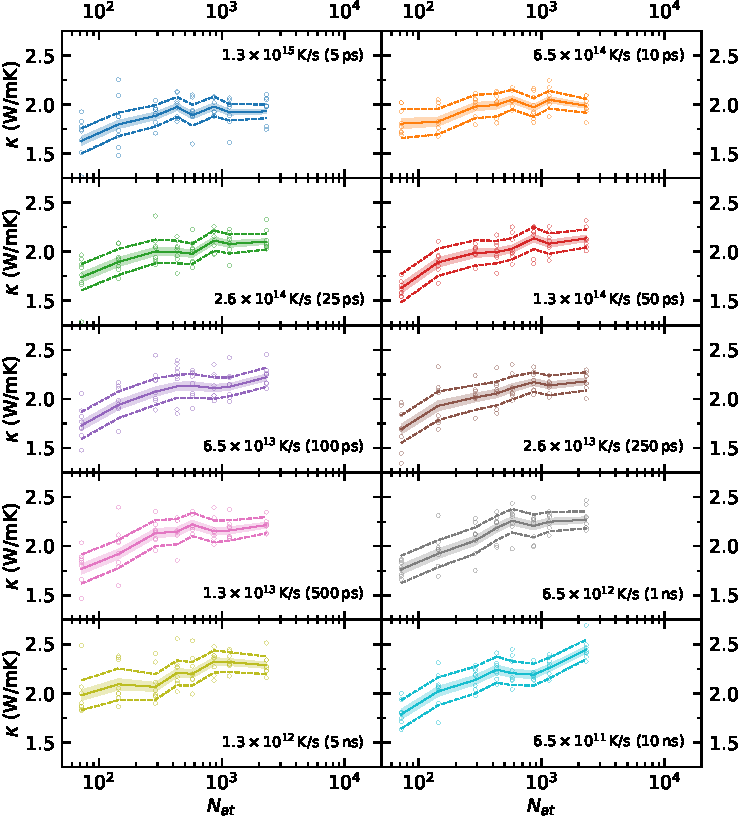
\includegraphics[width=\textwidth]{chapters/appendix/figures/Silica_NPT_kappa_NATconv_tesi.pdf}
    \caption{Thermal conductivity of a-SiO$_2$ at $500\un{K}$ obtained by a quench in the NPT ensemble at zero-pressure and with cooling rate $\gamma$. 
    The abscissa indicate the number of atoms of the system, each panel corresponds to a different quenching rate $\gamma$ (the relative quenching time $t_\mathrm{quench}$ is indicated in brackets). 
    The same symbols as Fig.~\ref{fig:results-class-kappa-vs-size} are used.
    }
    \label{fig:appendix-silica-class-npt-kappa-vs-size}
\end{figure}

\begin{figure}[!htb]
    \centering
    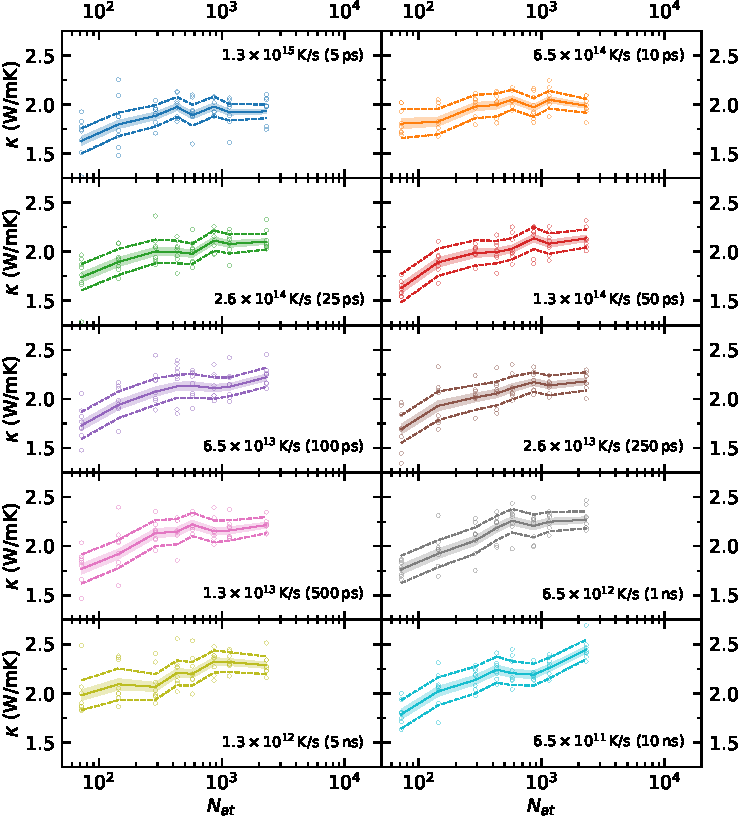
\includegraphics[width=\textwidth]{chapters/appendix/figures/Silica_NPT_kappa_NATconv_tesi.pdf}
    \caption{Thermal conductivity of a-SiO$_2$ at $500\un{K}$ obtained by a quench in the NPT ensemble at zero-pressure and with cooling rate $\gamma$. 
    Each panel corresponds to a different system size with $N_{at}$ atoms.
    The same symbols as Fig.~\ref{fig:results-class-kappa-vs-quench} are used.
    }
    \label{fig:appendix-silica-class-npt-kappa-vs-quench}
\end{figure}

\begin{figure}[!htb]
    \centering
    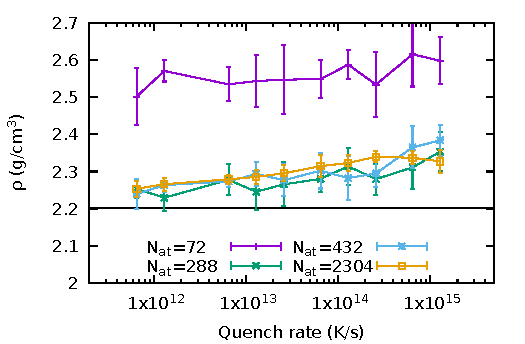
\includegraphics[width=12cm]{chapters/appendix/figures/dens_NPT_quench.pdf}
    \caption{Average density of a sample of $N_\mathrm{at}$ atoms at $500\un{K}$, obtained from a quench in the NPT ensemble at zero-pressure as a function of the quenching rate. The black line indicates the experimental value $\rho=2.202\un{g/cm^3}$. }
    \label{fig:appendix-silica-class-npt-density-vs-quench}
\end{figure}   % Appendix

%\bibliographystyle{unsrtnat}
%\bibliography{bibliography}
\printbibliography %[heading=bibintoc]

\end{document}